\documentclass[20pt,landscape]{extarticle}
%-----------------------------------------------------
%\newif\ifpdf
%\ifx\pdfoutput\undefined
%\pdffalse
%\else
%\pdfoutput=1
%\pdftrue
%\fi

%\ifpdf
\usepackage[pdftex]{graphicx}
\usepackage[pdftex, colorlinks=true, linkcolor=black]{hyperref}
%\else
%\usepackage{graphicx}
%\usepackage{hyperref}
%\fi

%-----------------------------------------------------
\usepackage{color}	% Farbverwaltung
\usepackage[english, ngerman]{babel} % Neue deutsche Rechtsschreibung
\usepackage[utf8]{inputenc}
%\usepackage[latin1]{inputenc} % Ermöglicht Umlaute-Darstellung
\usepackage{listings} % Code-Darstellung
\usepackage{ gensymb }
\lstset
{% general command to set parameter(s)
	basicstyle= \scriptsize, % print whole listing small
	keywordstyle=\bfseries,
	% underlined bold black keywords
	identifierstyle=, % nothing happens
	%commentstyle=\color{red}, % white comments
	stringstyle=\ttfamily, % typewriter type for strings
	showstringspaces=false, % no special string spaces
	framexleftmargin=7mm, 
	tabsize=3,
	showtabs=false,
	frame=single, 
	%rulesepcolor=\color{blue},
	numbers=left,
captionpos=b,
	linewidth=0.99\textwidth,%146mm,
	xleftmargin=8mm
}
\usepackage{amssymb,amsfonts,amstext,amsmath} % Mathematische Symbole
\usepackage[a4paper]{geometry}
\usepackage[german, ruled, vlined]{algorithm2e}
\usepackage{bibgerm}
\usepackage{makeidx}         % Erlaubt die Erzeugung eines Index-Verzeichnisses
\usepackage{multicol}        % Zweispaltiger Index-Verzeichnis
\usepackage[export]{adjustbox}
\usepackage{float}


\renewcommand*\familydefault{\sfdefault} 

\newtheorem{definition}{Definition}[section]
\newtheorem{algorithmus}{Algorithmus}[section]
\newtheorem{beispiel}{Beispiel}[section]
\newtheorem{satz}{Satz}[section]
\newtheorem{folgerung}{Folgerung}[section]
\newtheorem{theorem}{Satz}[section]

\pagestyle{myheadings} % Erzeugt selbstdefinierte Kopfzeile


\setlength{\headsep}{70pt}
\setlength{\textheight}{14cm}
\setlength{\textwidth}{1.2\textwidth}
\setlength{\oddsidemargin}{-0.01\textwidth}
\setlength{\evensidemargin}{-0.01\textwidth}

\title{Prozedurale Generierung von Baumstrukturen innerhalb der Unreal Engine 4}
%---- Die Art der Dokumentation kann hier ausgewählt werden---------------
%\project{Master Abschlussarbeit}
%\project{Master Projektstudium}
\project{Bachelor Abschlussarbeit}
%\project{Projektarbeit}
%\project{Seminar zur Vorlesung ...}
%\project{Präsentation zur Bachelor}
%--------------------------------------------------------------------------
\author{David Liebemann}
\date{17.03.17}





\begin{document}

% Titelseite
\mytitlepage

% neue Folie
\newpage
\noindent
{\Large \textbf{Überblick}} 
\slidetitle{}
\begin{enumerate}
	\item Einleitung 
	\item Lindenmayer-Systeme
	\item Space Colonization Algorithmus
	\item Implementierung
	\item Ergebnisse
	\item Zusammenfassung und Ausblick
\end{enumerate}
\newpage
\slidetitle{}
\section{Einleitung}
\begin{center}
	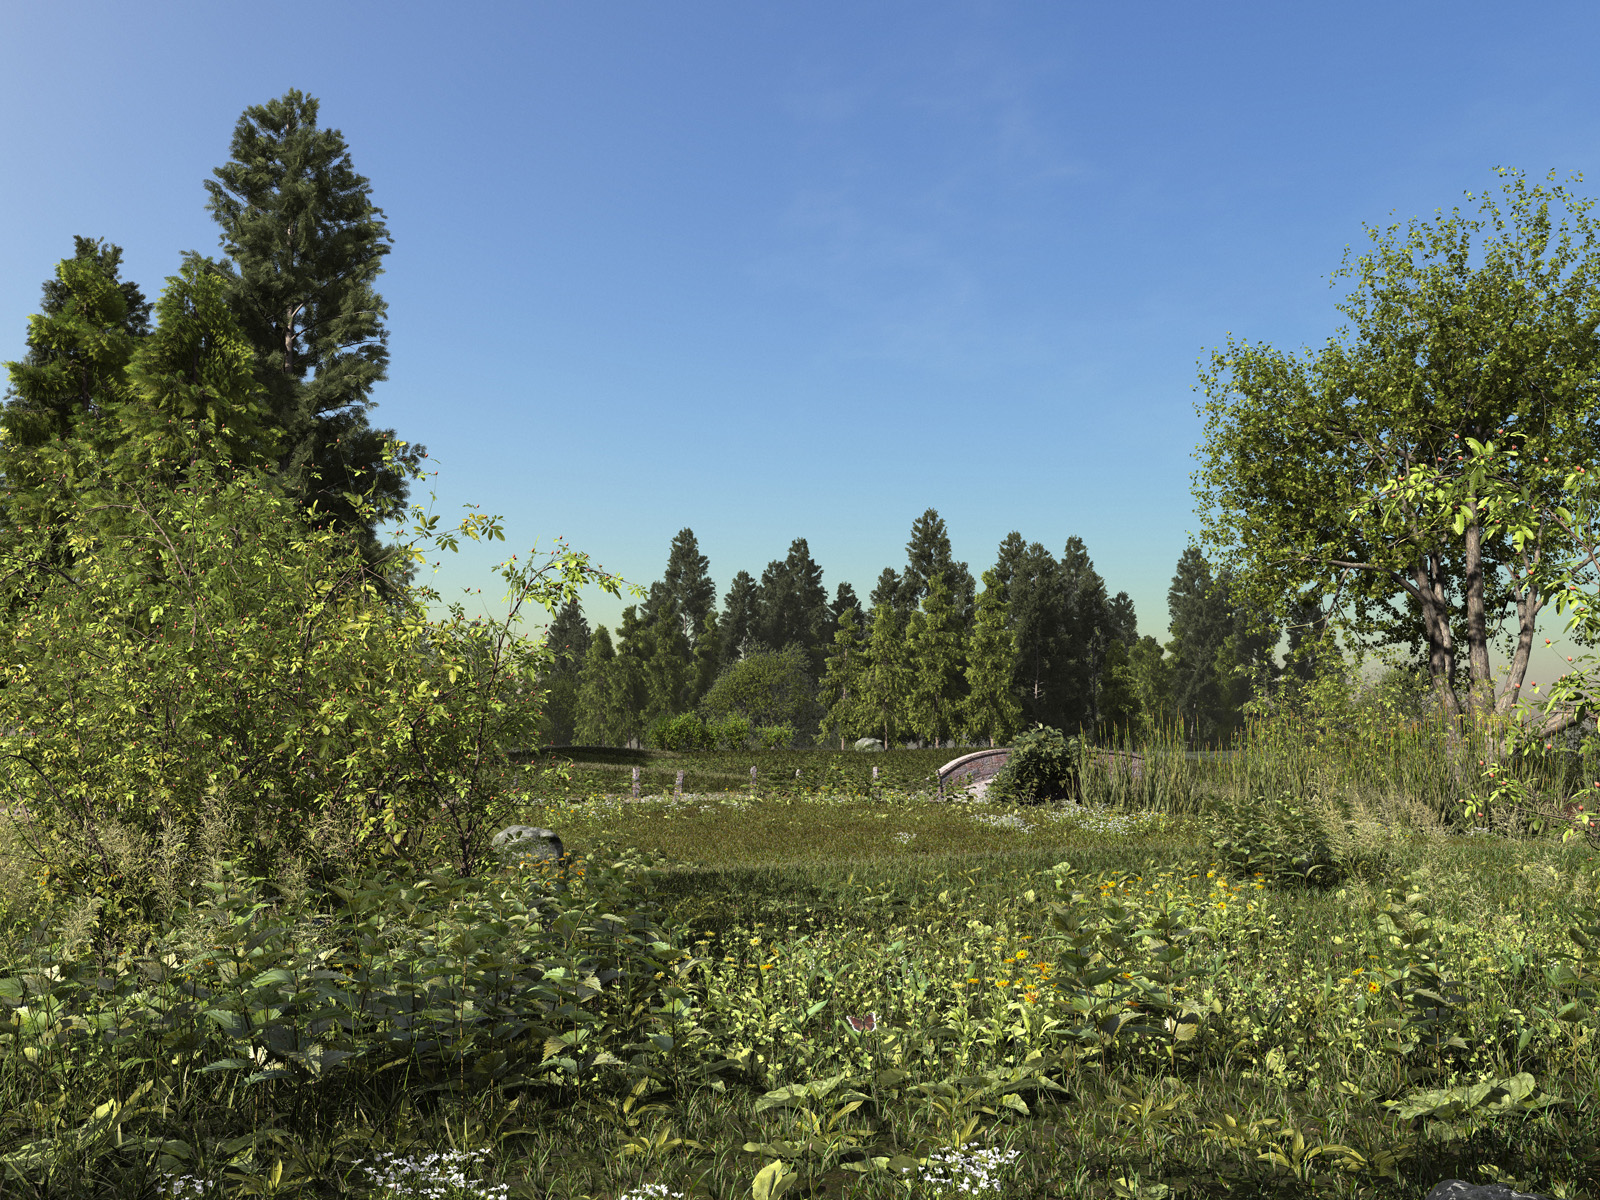
\includegraphics[height=.85\textheight]{images/CH1_greenXfrog_JanWalterSchliep.jpg}
	\cite{GreenOne:16}
\end{center}

%\paragraph{Prozedurale Generierung\\}
%\begin{itemize}
%	\item Konstruktion von 3D-Modellen mithilfe computergenerierter Daten\\
	
%	\item Benötigt lediglich eingeschränkten Eingriff durch Benutzer\\
	
%	\item Generierung von Pflanzenmodellen
%\end{itemize}


\newpage
\slidetitle{1. Einleitung - Ansatz}
\paragraph{Ansatz\\}

\begin{itemize}
	\item Implementierung von zwei Verfahren zur prozeduralen Generierung von Baumstrukturen:
	\begin{itemize}
		\item Lindenmayer-Systeme
		\item Space Colonization Algorithmus\\
	\end{itemize}
	\item Verwendung des Frameworks \glqq Unreal Engine 4\grqq\\
	
	\item Vereinfachte Darstellung von Ästen in Form von Zylindern
\end{itemize}

\newpage
\slidetitle{1. Einleitung - Unreal Engine 4}
\paragraph{Unreal Engine 4\\}

\begin{itemize}
	\item Sammlung von Softwarewerkzeugen \\
	
	\item Erstellung von Inhalten mit C++ oder Blueprint und auf Basis von Framework-Klassen\\
	
	\item Verfügbarkeit eines visuellen Editor erlaubt:
	\begin{itemize}
		\item Einfache Positionierung von Actors
		\item Eingabe von Parametern über das Editor-UI
	\end{itemize}
\end{itemize}

\iffalse

\newpage
\begin{center}
	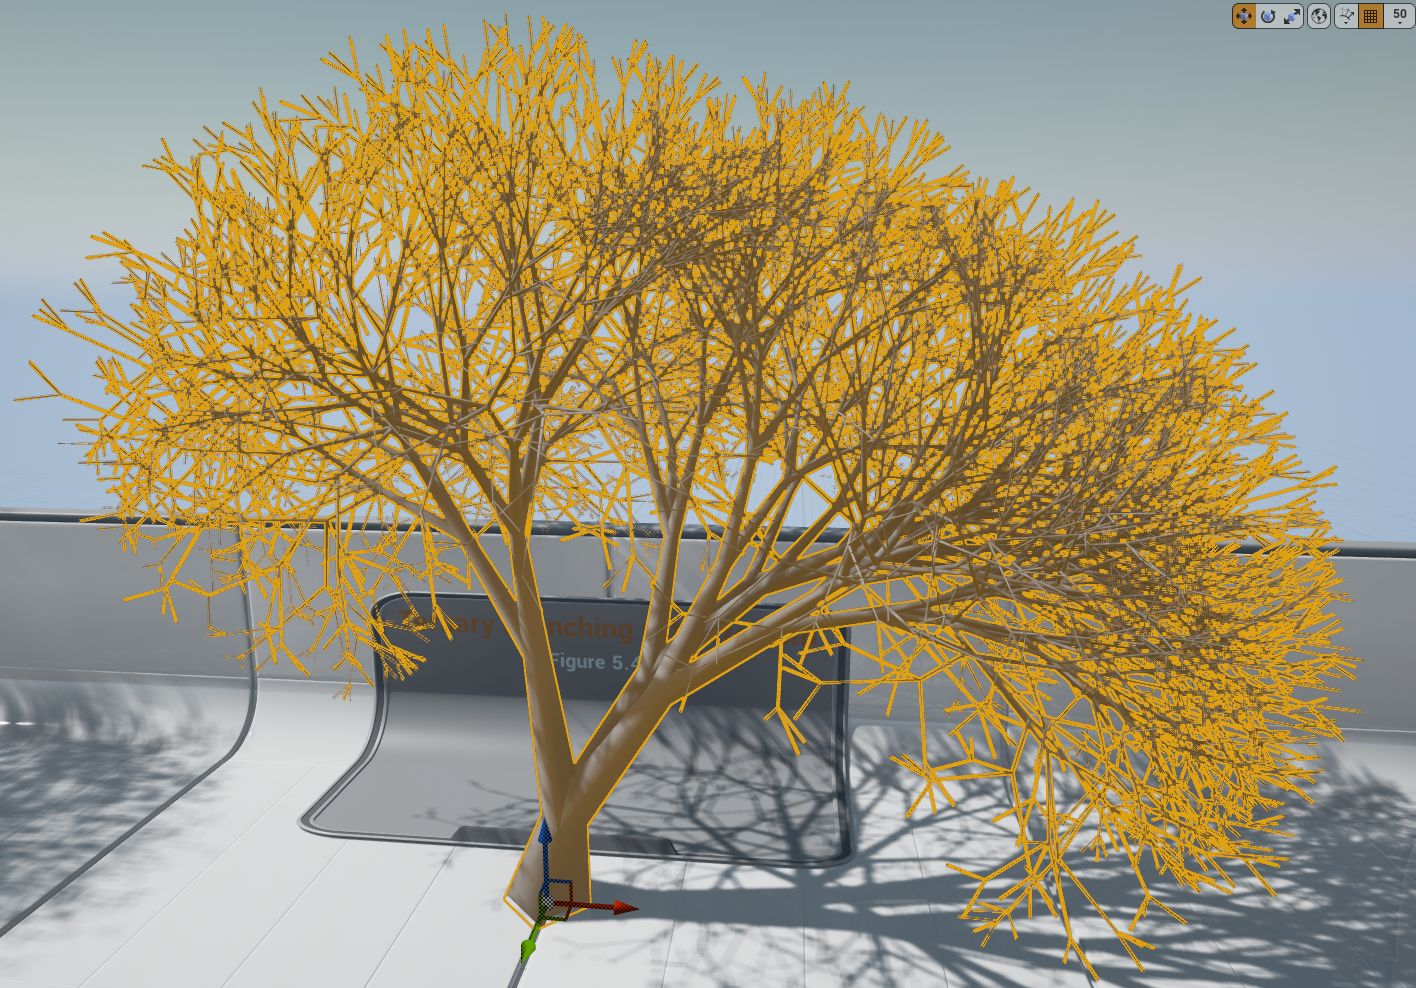
\includegraphics[height=0.9\textheight]{images/CH1_EditorExample1.png}
	
	Positionierung eines Actors im Leveleditor
\end{center}

\begin{center}
	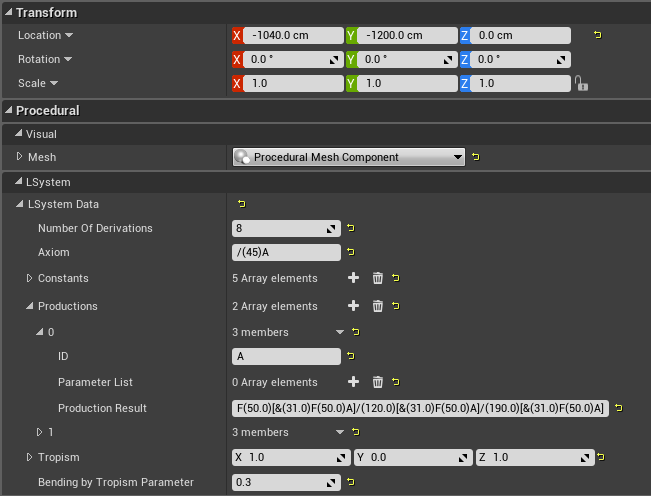
\includegraphics[height=0.9\textheight]{images/CH1_EditorExample2.png}
	
	Eingabefenster für Actor-Parameter
\end{center}



\newpage
\slidetitle{1. Einleitung - Bisherige Arbeiten}
\paragraph{Bisherige Arbeiten}
\begin{center}
	\begin{minipage}[c]{0.45\textwidth}
		\centering
		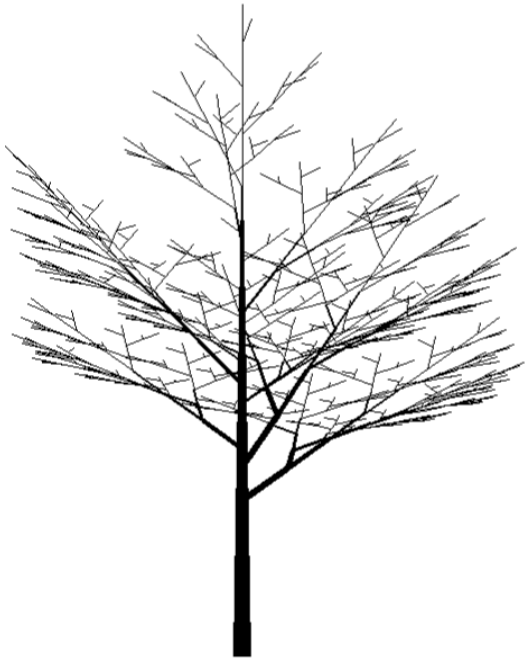
\includegraphics[height=0.6\textheight]{images/CH1_Honda1.png}
		
		Honda und Fisher \cite{ABOP:04}
	\end{minipage}
	\hspace{.05\textwidth}	
	\begin{minipage}[c]{0.45\textwidth}
		\centering
		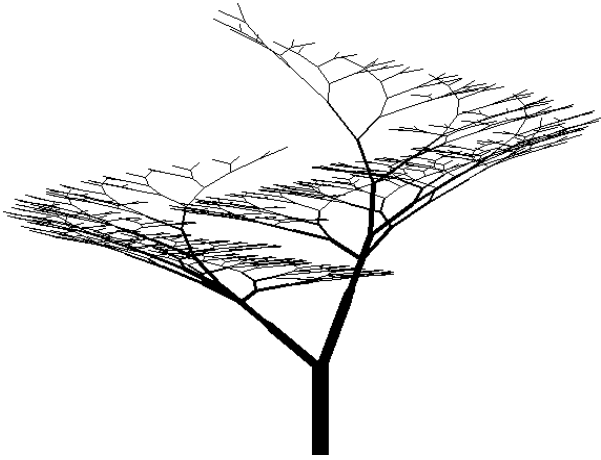
\includegraphics[height=0.6\textheight]{images/CH1_AonoKunii1.png}
		
		Aono und Kunii \cite{ABOP:04}
	\end{minipage}
\end{center}


\begin{center}
	\vfill
	\begin{minipage}[c]{0.45\textwidth}
		\centering
		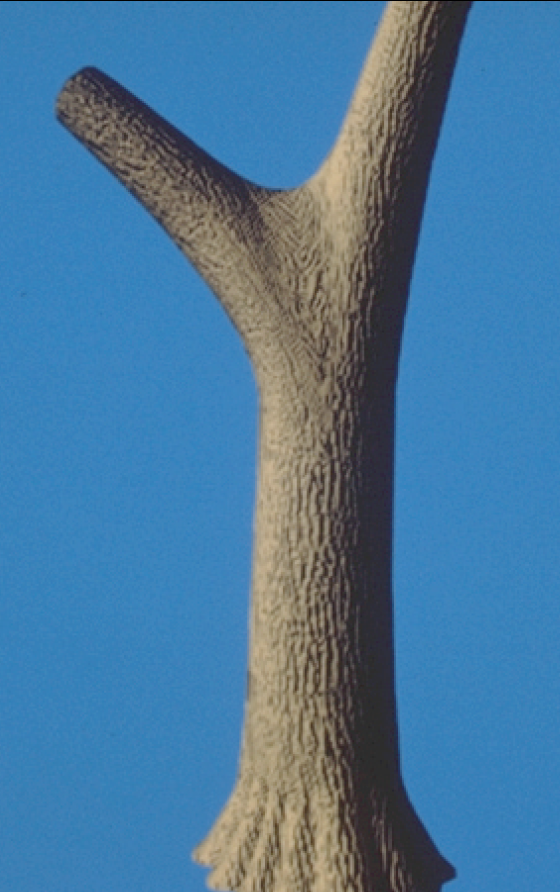
\includegraphics[height=0.6\textheight]{images/CH1_Bloomenthal1.png}
		
		Bloomenthal \cite{ABOP:04}
	\end{minipage}
	\hspace{.05\textwidth}	
	\begin{minipage}[c]{0.45\textwidth}
		\centering
		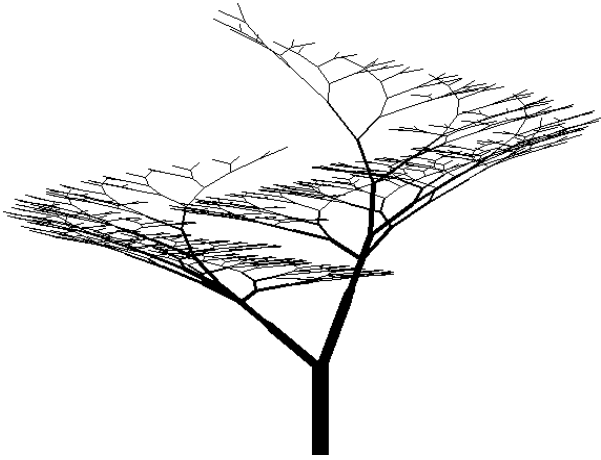
\includegraphics[height=0.6\textheight]{images/CH1_AonoKunii1.png}
		
		Aono und Kunii \cite{ABOP:04}
	\end{minipage}
\end{center}
\fi


	


% neue Folie
\newpage
\slidetitle{}
\section{Lindenmayer-Systeme \\}

\begin{itemize}
	\item Von Aristid Lindenmayer 1968 entwickelte Erweiterung von Ersetzungssystemen \\
	
	\item Weitere Ergänzungen durch Prusinkiewicz und Lindenmayer in 1990\\
	
	\item Funktionsweise basiert auf der Ersetzung von Zeichen in Zeichenketten \\
	
	\item Grafische Interpretation der Resultate ergibt Modelldaten
	
\end{itemize}





\newpage
\slidetitle{2. L-Systeme - D0L-Systeme}

\subsection{D0L-Systeme\\ }
\newtheorem{defD0LSystem}{Definition D0L-System:}[subsection]
\begin{defD0LSystem}
	Ein deterministisches, kontextfreies L-System (D0L-System) ist ein Tupel G = $(V, P, \omega)$ mit:
	
	\begin{description}
		\item[\boldmath$V:$ ] Ein nichtleeres, endliches Alphabet\\
		
		\item[\boldmath$P:$ ] Eine Menge von Produktionsregeln in der Form $p_1: a \rightarrow b$ mit $a \in V$ und $b \in V^*$ \\
		
		\item[\boldmath$\omega \in V^+ :$ ]  Das Axiom, Startwort des L-Systems		
	\end{description}
\end{defD0LSystem}





\newpage

\paragraph{Verwendete Begriffe:\\}

\begin{description}
	\item[\textbf{Deterministisch:}] Es existiert genau eine Produktionsregel für jedes der Symbole in $V$ \\
	
	\item[\textbf{Kontextfrei:}] Ersetzung findet unabhängig von umgebenden Symbolen statt \\
	
	\item[\textbf{Ableitung:}] Gleichzeitige Ersetzung aller Symbole eines Wortes anhand der Produktionsregeln
	
\end{description}





\newpage
\slidetitle{2. L-Systeme - D0L-Systeme}

\paragraph{Beispiel: Simulation des Wachstums der Blaualgen-Gattung \glqq Anabaena\grqq{} \\}

  
\begin{description}
	\item[\boldmath$V$]  besteht aus den Symbolen \boldmath$\{a_l, a_r, b_l, b_r\}$
	\begin{description}
		\item[\boldmath$a$ und \boldmath$b$:] Größe und Teilungsbereitschaft einer Zelle\\
		\item[\boldmath$l$ und \boldmath$r$:] Zellenpolarität
	\end{description}
	\item[\boldmath$P$] besteht aus:
	\begin{description}
		\item[\boldmath$p_1 :$] $\begin{array}{ccc} a_r & \rightarrow & a_lb_r \end{array}$
		\item[\boldmath$p_2 :$] $\begin{array}{ccc} a_l &\rightarrow& b_la_r \end{array}$
		\item[\boldmath$p_3 :$] $\begin{array}{ccc} b_r &\rightarrow& a_r \end{array}$
		\item[\boldmath$p_4 :$] $\begin{array}{ccc} b_l &\rightarrow& a_l  \end{array}$
	\end{description}
\end{description}





\newpage

\begin{center}
	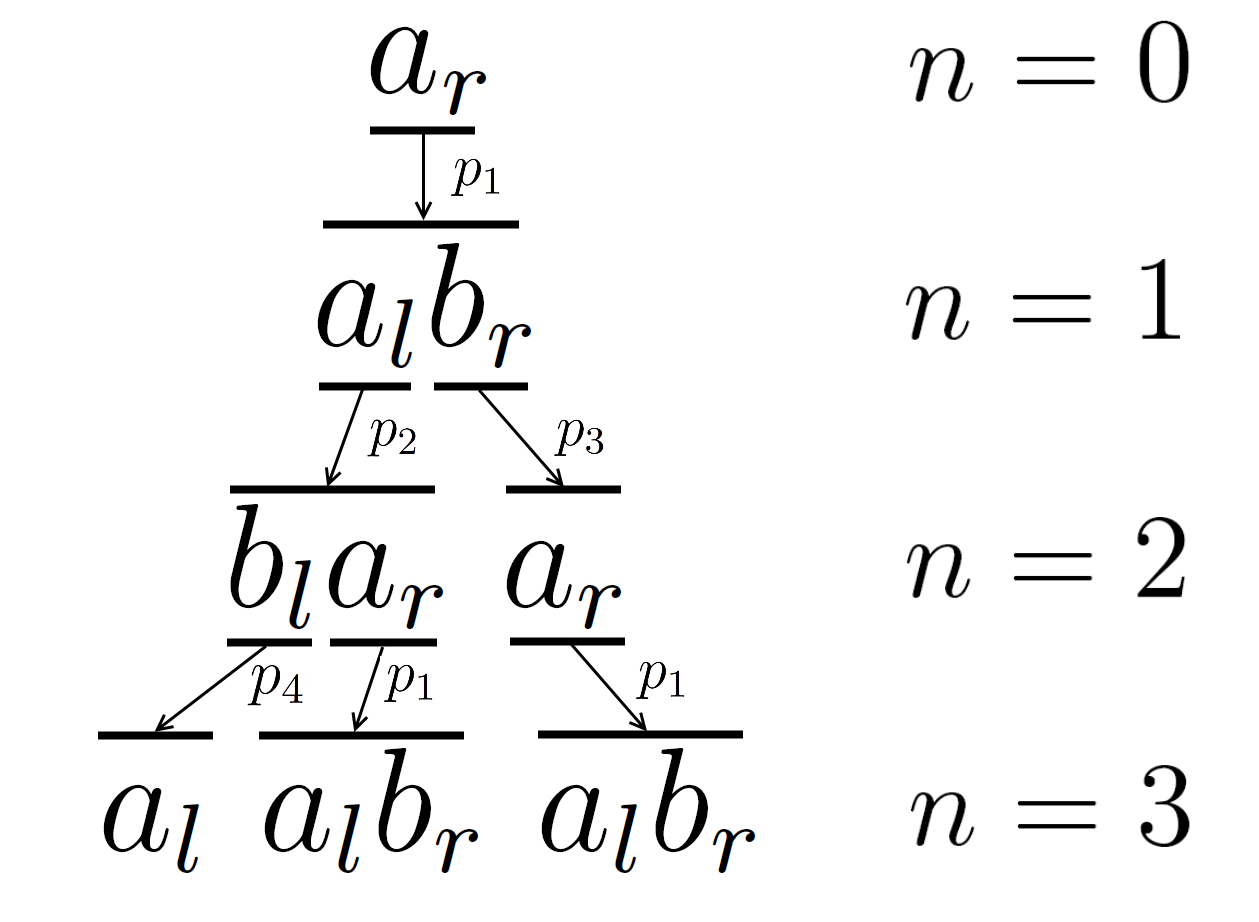
\includegraphics[height=1\textheight]{images/CH2_AnabaenaAbleitung.png}
\end{center}





\newpage
\slidetitle{2. L-Systeme - parametrische L-Systeme}
\subsection{Parametrische L-Systeme\\ }

\begin{itemize}
	\item Erweiterung der D0L-Systeme \\
	
	\item Verwendung von parametrischen Wörtern anstatt einfacher Symbole:
	\begin{description}
			\item[\boldmath$A(a_1, ..., a_n):$] Parametrisches Wort mit $A\in V$ und $a_1, ..., a_n \in \Sigma$\\
		
			\item[\boldmath$\Sigma:$] Menge formaler Parameter\\
	\end{description}
	
	\item Verwendung arithmetischer Ausdrücke im Nachfolger möglich
	%\begin{description}
		
	%	\item[\boldmath$E(\Sigma):$] Arithmetischer Ausdruck
	%\end{description}

\end{itemize}




\iffalse
\newpage
\paragraph{}
\newtheorem{defParametrischeLSysteme}{Parametrisches L-System:}[subsection]
\begin{defParametrischeLSysteme}
	Ein Parametrisches L-System ist ein Tupel G = $(V, \Sigma, P, \omega)$ mit:
	\begin{description}
		\item[\boldmath$V:$] Ein nichtleeres, endliches Alphabet\\
		
		\item[\boldmath$\Sigma:$] Eine Menge formaler Parameter\\
		
		\item[\boldmath$P:$] Eine Menge von Produktionsregeln $P : (V\times \Sigma^*) \rightarrow (V\times E(\Sigma)^*)^*$\\
		
		\item[\boldmath$\omega \in M^+$] mit $M =(V \times \mathbb{R}^*)$ -- das Axiom in Form eines nichtleeren, parametrischen Wortes
	\end{description}
\end{defParametrischeLSysteme}
\fi




\newpage
\paragraph{Beispiel: Definition und Ableitung eines parametrischen L-Systems \\}

\begin{equation}
\begin{array}{llll}
\omega & : A(1,1) \\
p_1 & : A(x,y) &\rightarrow& A(x+1, y*2)\text{ }B(y) \\
p_2 &  : B(z) &\rightarrow& B(z+1)\text{ }C 
\end{array}
\label{eq:ProdParamLSystem}
\end{equation} 


\begin{description}
	\item[\boldmath$V$ ]  $= \{A,B,C\}$\\
	
	\item[\boldmath$\Sigma$ ] $= \{x,y,z\}$\\
	
	\item[\boldmath$P$ ] $= \{p_1, p_2\}$\\
	
	\item[\boldmath$\omega$ ]  $= A(x,y)$ mit $x=1$ und $y=1$
\end{description}





\newpage
\begin{center}
	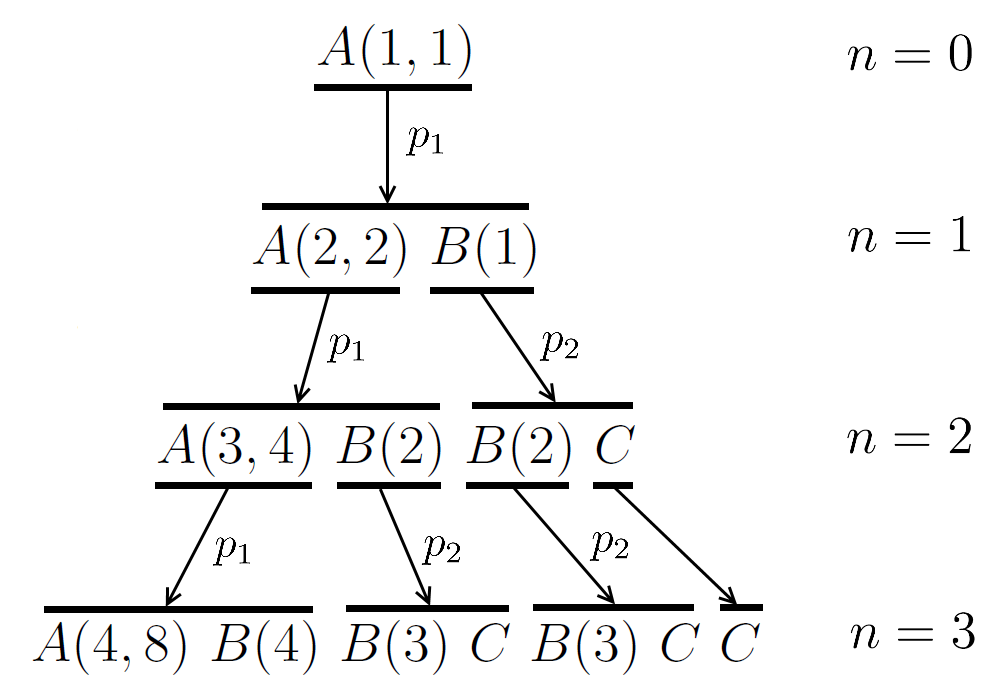
\includegraphics[height=1\textheight]{images/CH2_ParamLSystemBeispiel.png}
\end{center}




\newpage
\slidetitle{}
\subsection{Grafische Interpretation von L-Systemen\\}

\begin{itemize}
	\item Rückgabewerte von L-System-Ableitungen sind Zeichenketten, keine Modelldaten\\
	
	\item Grafische Interpretation von Zeichenketten: Turtle-Interpretation\\
	
	\item Zustand der Turtle ist ein Tupel $(\overrightarrow{p}, \overrightarrow{H})$ mit:
	\begin{description}
		\item[\boldmath$\overrightarrow{p}:$] Position der Turtle\\
		
		\item[\boldmath$\overrightarrow{H}:$] Blickrichtung (Heading) der Turtle
	\end{description}
\end{itemize}






\newpage
\slidetitle{2. L-Systeme -- Grafische Interpretation}

\paragraph{Turtle-Aktionen: \\}

\begin{description}
	\item[\boldmath$F(l):$] Bewegung um $l>0$ in Blickrichtung, Aktualisierung der Position und Zeichnung einer Linie\\
	
	\item[\boldmath$+(d):$]  Drehung um den Winkel $d$ nach links, Aktualisierung der Blickrichtung\\
	
	\item[\boldmath$-(d):$] Drehung um den Winkel $d$ nach rechts, Aktualisierung der Blickrichtung\\
	
	\item[\boldmath$[ \text{ }:$] Ablage des Zustands auf einem Stack\\
	
	\item[\boldmath$\mathbf{]} \text{ }:$] Entnahme des obersten Zustands vom Stack und Aktualisierung des aktuellen Zustands
	
\end{description}




\newpage
\begin{center}
	\begin{minipage}[c]{0.45\textwidth}
		\centering
		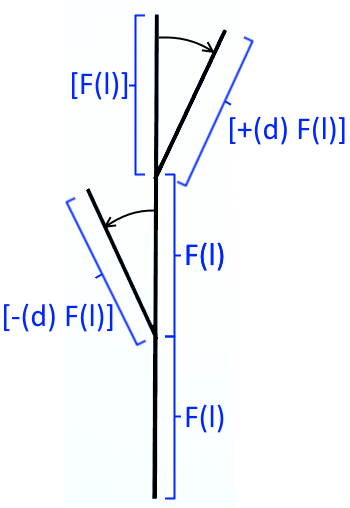
\includegraphics[height=.75\textheight]{images/CH2_Branching2_N1L15D25.png}
		
		$n=1$, $l=240$, $d=25\degree$
	\end{minipage}
	\begin{minipage}[c]{0.45\textwidth}
		\centering
		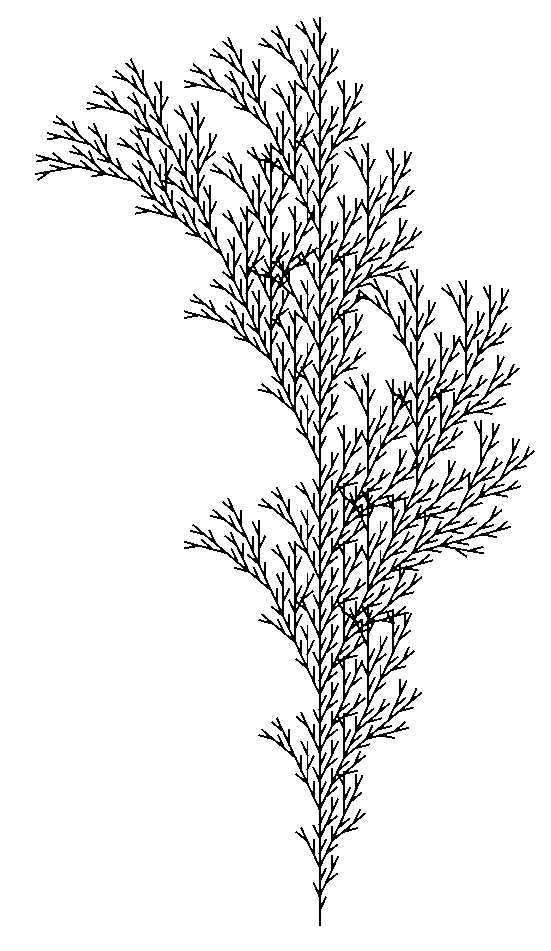
\includegraphics[height=.75\textheight]{images/CH2_Branching2_N5L15D25.png}
		
		$n=5$, $l=15$, $d=25\degree$
	\end{minipage}
	\vspace{0.075\textheight}
	
	$\begin{array}{ll}
	\omega & : F(l) \\
	p_1 & : F(l) \rightarrow F(l)\text{ }[+(d)\text{ }F(l)]\text{ }F(l)\text{ }[-(d)\text{ }F(l)]\text{ }[F(l)]
	\end{array}$
\end{center}



\newpage
\slidetitle{2. L-Systeme -- Anpassungen: 3D Turtle-Interpretation}

\subsection{Anpassungen an Baumstrukturen \\}

\paragraph{Erweiterung der Turtle-Interpretation in den dreidimensionalen Raum}

\begin{itemize}
	\item Zustand der Turtle ist ein Tupel $(\overrightarrow{p}, \boldsymbol{R})$ mit:
	\begin{description}
		\item[\boldmath$\overrightarrow{p}:$] Position der Turtle
		
		\item[\boldmath$\boldsymbol{R}:$] Rotationsmatrix der Turtle\\
	\end{description}
	
	\item Einheitsvektoren $\overrightarrow{H}, \overrightarrow{L}, \overrightarrow{U}$ bilden das lokale Koordinatensystem der Turtle:
	\begin{description}
		\item[\boldmath$\overrightarrow{H}:$] Heading-Vektor
		
		\item[\boldmath$\overrightarrow{L}:$] Left-Vektor
				
		\item[\boldmath$\overrightarrow{U}:$] Up-Vektor
	\end{description}
\end{itemize}





\newpage
\begin{center}
	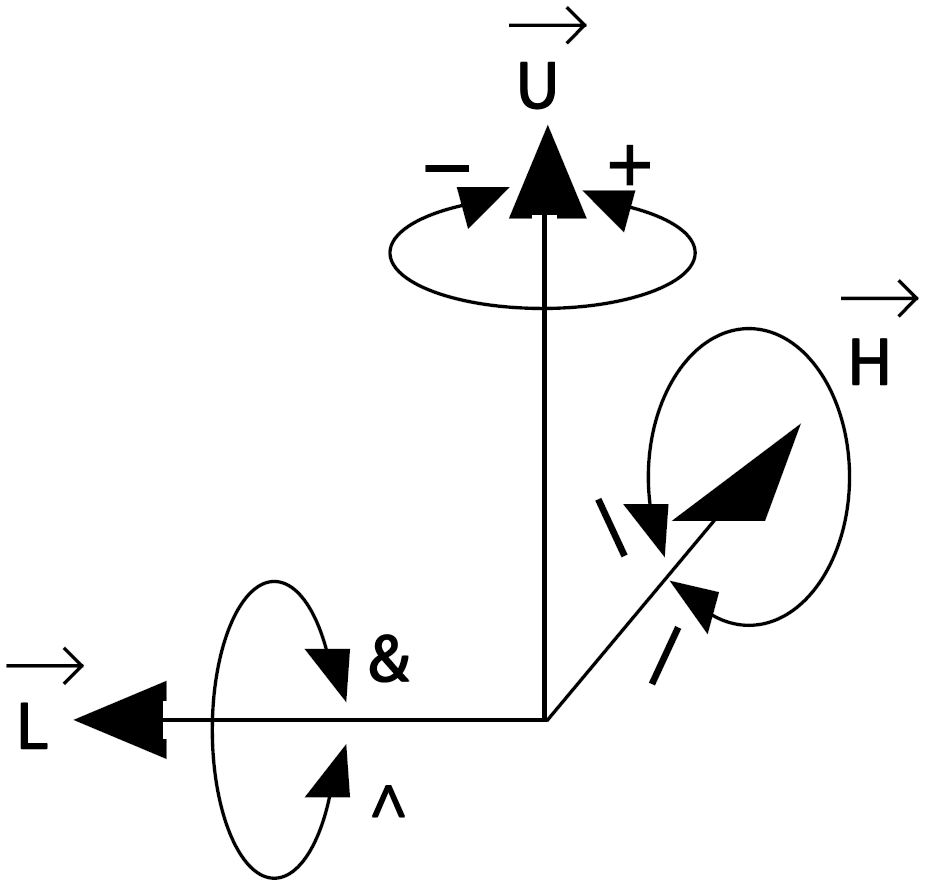
\includegraphics[height=1\textheight]{images/CH2_Turtle3D.png}
	\cite[S.19]{ABOP:04}
\end{center}





\newpage
\begin{center}
	\begin{minipage}[c]{0.6\textwidth}
		\centering
		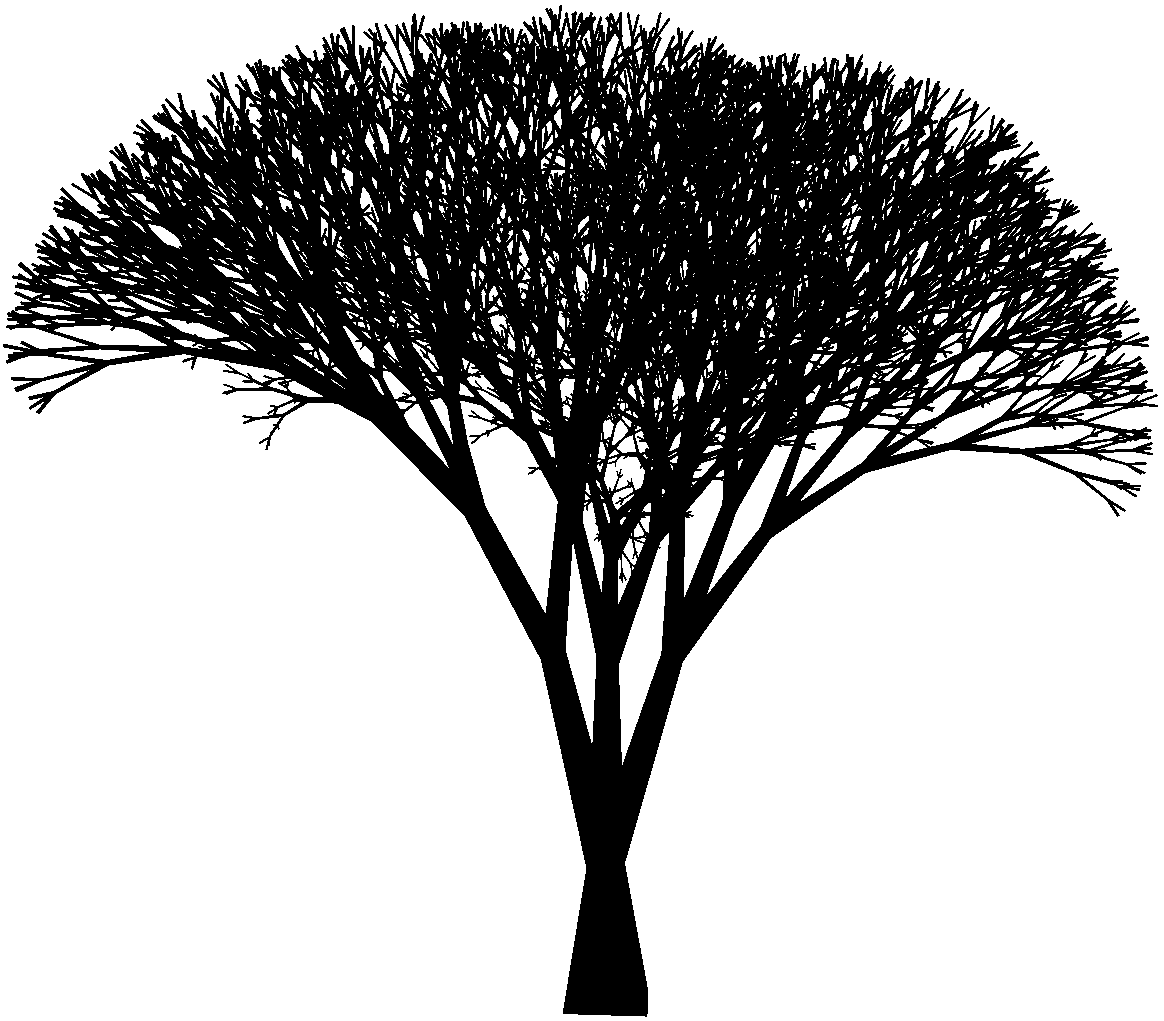
\includegraphics[height=.75\textheight]{images/CH2_3DTreeP61B_Angle_18_95.png}
	\end{minipage}
	\begin{minipage}[c]{0.35\textwidth}
			$n=8$, $l=50$, $d=137.5\degree$, 
			
			$a=18.95\degree$, $l_r = 1.3$
	\end{minipage}
\end{center}

\begin{equation}
\begin{array}{llll}
\omega :&  /(45)\text{ }A \\
p_1 :&  A &\rightarrow & F(l)\text{ }[\&(a)F(l)A]\text{ }/(d)\text{ }[\&(a)F(l)A]\text{ }/(d)\text{ }[\&(a)F(l)A] \\
p_2 :& F(l) &\rightarrow & F(l*l_r)
\end{array}
\end{equation}




\newpage
\slidetitle{2. L-Systeme -- Anpassungen: Tropismus}

\paragraph{Einfluss durch Tropismus\\}


\begin{itemize}
	\item Tropismus:Tendenz einer Pflanze in eine bestimmte Richtung zu wachsen\\
	
	\item Einfluss wird als Vektor $\overrightarrow{T} \in \mathbb{R}^3$ angegeben \\
	
	\item Beeinflusst die Bewegung der Turtle in Abhängigkeit des Beugungsfaktors $e \in \mathbb{R}$
\end{itemize}





\newpage
\begin{center}
	
	\begin{minipage}[c]{0.55\textwidth}
		\centering
		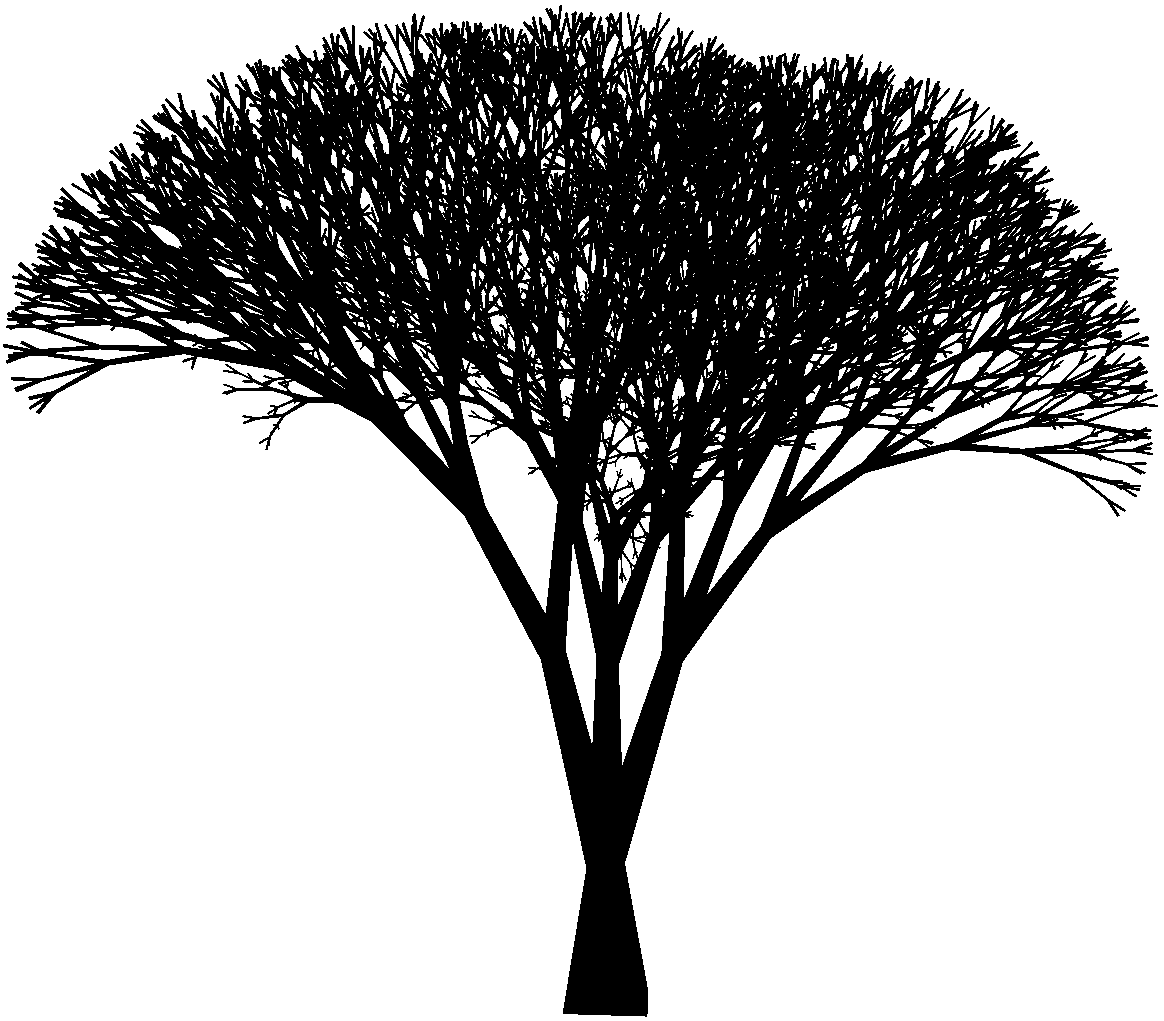
\includegraphics[height=.75\textheight]{images/CH2_3DTreeP61B_Angle_18_95.png}
		\vspace{0.05\textheight}
		
		$\overrightarrow{T} =\begin{pmatrix}
		0 \\ 0 \\ 0
		\end{pmatrix}$, $e = 0$
	\end{minipage}
	\begin{minipage}[c]{0.4\textwidth}
		\centering
		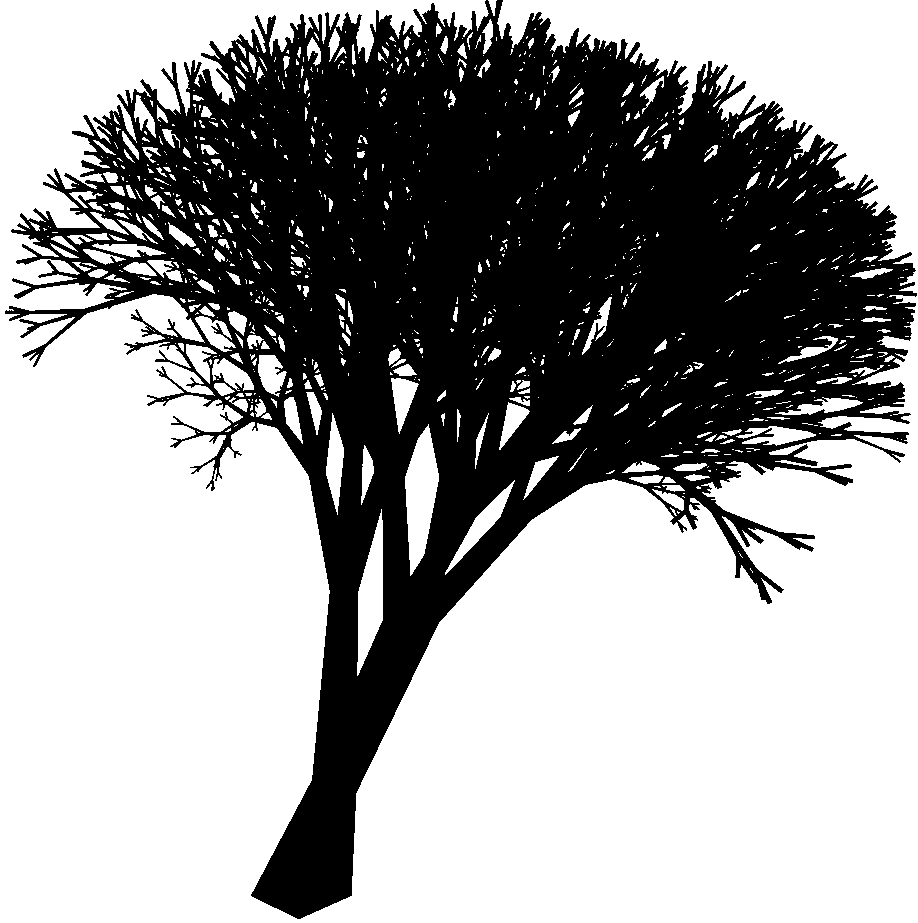
\includegraphics[height=.75\textheight]{images/CH2_3DTreeP61B_Angle_18_95_Tropism.png}
		\vspace{0.05\textheight}
		
		$\overrightarrow{T} =\begin{pmatrix}
		0 \\ 1 \\ -0.5
		\end{pmatrix}$, $e = 0.27$
	\end{minipage}
\end{center}



\iffalse

\newpage
\slidetitle{2. L-Systeme -- Anpassungen: Graphentheoretischer Baum}

\paragraph{Repräsentation der Turtle-Aktionen als graphentheoretischer Baum\\}

\begin{itemize}
	\item Turtle-Interpretation baut einen graphentheoretischen Baum $G=\langle V,E\rangle$ auf\\
	
	\item Jeder Knotenpunkt $v\in V$ entspricht einem Punkt $\overrightarrow{p}_v \in \mathbb{R}^3$\\
	
	\item Jeder Knotenpunkt besitzt maximal einen Vorgänger und eine endliche Menge von Nachfolgern \\
		
	\item Zustand der Turtle ist ein Tupel $(\overrightarrow{p}, v, \boldsymbol{R})$ mit $v\in V$ \\
	
\end{itemize}




\newpage
\begin{itemize}
	\item Erweiterung der Turtle-Bewegung \boldmath$F(l)$ ausgehend von Zustand $(\overrightarrow{p}, v, \boldsymbol{R})$:
	\begin{itemize}
		\item Bewegung zu Position $\overrightarrow{p_{neu}}$\\
		
		\item Erstellung eines Knotens $v_{neu}$ und einer Kante $(v, v_{neu})$\\
		
		\item Neuer Turtle-Zustand: $(\overrightarrow{p_{neu}}, v_{neu}, \boldsymbol{R})$\\
	\end{itemize}
\end{itemize}

\fi


\newpage
\slidetitle{}
\section{Space Colonization Algorithmus}
\subsection{TODO}

\begin{center}
%	\includegraphics[width=0.52\textwidth]{}
\end{center}

\newpage
\slidetitle{3. Space Colonization Algorithmus - TODO}

\begin{itemize}
\item TODO \\

\end{itemize}



\chapter{Implementierung}


Im folgenden Kapitel wird die Implementierung der Vorgehen innerhalb des Frameworks der Unreal Engine 4 behandelt. Die Baumrepräsentation enthält Daten, die von den L-System und Space Colonization Implementierungen generiert werden. Diese Daten werden an das Modellgenerierungssystem übergeben, welches die Modelldaten für eine grafische Darstellung in der Unreal Engine 4 produziert.


\section{Baumrepräsentation}

Sowohl L-Systeme als auch der Space Colonization Algorithmus generieren einen graphentheoretischen Baum, auf dessen Grundlage die Modellgenerierung durchgeführt wird. Die implementierte Baumrepräsentation kann daher von beiden Systemen verwendet werden und ermöglicht es, diese mit demselben Modellgenerierungssystem zu visualisieren.

Der Baum wird durch eine Datenklasse repräsentiert, jedes Objekt dieser Klasse beschreibt einen Knoten sowie die Kante, welche vom Vorgänger zu dem Knoten führt. Die Datenklasse bietet Zugriff auf die folgenden Informationen:

\begin{description}
	\item \textbf{Vorgänger und Nachfolger:} Mithilfe eines Verweises auf den Vorgänger und eine Liste der Nachfolger eines Knotens kann der Baum-Graph vollständig repräsentiert werden. Weiterhin ermöglicht dies die Implementierung einer Reihe von rekursiven Funktionen zur Anpassung von Modelldaten.\\
	
	\item \textbf{Modell-Daten:} Kanten werden, wie in Abschnitt \ref{subsec:ZylinderMeshes} beschrieben, mithilfe von Zylindern visualisiert. Um die Generierung von Modelldaten zu vereinfachen, bietet die Datenklasse Zugriff auf Start- und Endposition, Start- und Endradius, Start- und Endnormale sowie einen Rotationswinkel. 
	
	Des Weiteren wird die Zweigtiefe des repräsentierten Knoten gespeichert.\\
	
	\item \textbf{Wachstums-Daten:} Die Wachstums-Daten bestehen aus einer Wachstumsrichtung, einem Einfluss-Zähler und dem \glqq Kein Wachstum\grqq-Zähler ($NG$-Counter), welche für den Ablauf des Space Colonization Algorithmus benötigt werden.	
\end{description}

Ein Objekt der Datenklasse kann als Astsegment eines biologischen Baumes angesehen werden und wird durch das Modellgenerierungssystem als solches visualisiert. Im Folgenden wird der Begriff \glqq Astsegment\grqq{} verwendet, um ein Objekt der Datenklasse der Baumrepräsentation zu bezeichnen.

\section{L-Systeme}

Die Implementierung der Funktionsweise von L-Systemen wird durch einen Unreal-Actor verwirklicht, der im Level platziert werden kann. Nach Start des Levels wird das angegebene Axiom anhand der Produktionsregeln abgeleitet und die sich ergebende Zeichenkette von der Turtle-Implementierung interpretiert.

\subsection{Parameter}

Dem L-System-Actor werden die folgenden Parameter über die Editor-UI übergeben:

\begin{description}
	\item \textbf{Anzahl der Ableitungen:} Die Anzahl der Ableitungen in $\mathbb{N}^+$, welche auf dem Axiom durchgeführt werden. \\
	
	\item \textbf{Axiom:} Das Axiom in Form einer Zeichenkette. \\
	
	\item \textbf{Konstanten:} Eine Konstante besteht aus der Angabe eines Identifikationssymbols und eines Wertes in $\mathbb{R}$. Konstanten können im Axiom und in den Nachfolgern der Produktionen verwendet werden.\\	
	
	\item \textbf{Produktionen:} Jede Produktion besteht aus Angabe eines Vorgängers, eine Liste von Parametern und einem Nachfolger. Der Vorgänger und jeder Parameter entspricht einem einzelnen Symbol, der Nachfolger wird als Zeichenkette eingetragen. Die Parametersymbole können nur innerhalb des Nachfolgers verwendet werden. Der Vorgänger und die Liste der Parameter bilden das parametrische Wort, welches bei einer Ableitung durch den Nachfolger ersetzt wird. \\
	
	\item \textbf{Tropismus:} Der Einfluss von Tropismus in Form eines dreidimensionalen Vektors und eines Biegsamkeitsfaktors.
\end{description}
\begin{figure} [hbtp]
	\centering
	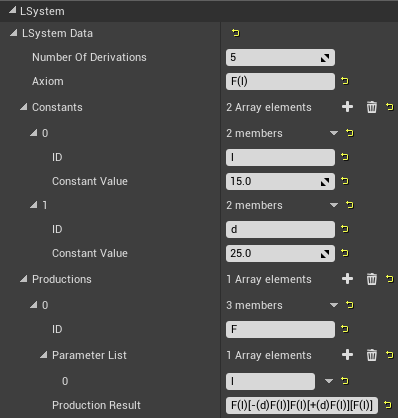
\includegraphics[height=0.4\textheight]{images/LS_ExampleUE4UI.png}
	\caption{Ein Beispiel für die Angabe des L-Systems aus Gleichung \ref{eq:ProdBranching2} mit der resultierenden Baumstruktur aus Abbildung \ref{fig:Branching2L15D25}.}
	\label{fig:LS_ExampleUE4UI}
\end{figure}
Für das Axiom und die Produktionen gelten die in Kapitel \ref{ch:LSysteme} festgelegten Regeln für die Definition von L-Systemen. Weiterhin gelten die Regeln für die Angabe von arithmetischen Operationen. Die Verwendung von Klammern ist jedoch auf die Angabe von Parametern eines parametrischen Wortes beschränkt, ihre Verwendung zur Beeinflussung der Auswertungsreihenfolge eines arithmetischen Ausdrucks wird nicht unterstützt.

Ein Beispiel für die korrekte Eingabe eines L-Systems über die Editor-UI wird in Abbildung \ref{fig:LS_ExampleUE4UI} gezeigt.

\subsection{Ableitung}

Zu Anfang der Erstellung des L-System-Actors werden alle Konstantensymbole im Axiom und den Produktionen durch die Konstantenwerte ersetzt. 

Die Implementierung arbeitet durchgehend auf derselben Zeichenkette, angefangen mit dem Axiom. In jeder Ableitung werden die in den Produktionsregeln definierten parametrischen Wörter durch die angegebenen Nachfolger ersetzt.

Nachdem die vorgegebene Anzahl von Ableitungen durchgeführt wurde, wird die resultierende Zeichenkette an die Turtle-Implementierung weiter gegeben.

\subsection{Turtle Interpretation} \label{subsec:TurtleInterpretationImplementation}

Der Turtle-Implementierung wird die aus den Ableitungen resultierende Zeichenkette übergeben. Diese wird daraufhin sequentiell abgearbeitet und entsprechend den in Abschnitt \ref{sec:LS_Baumstrukturen} vorgestellten Konzepten interpretiert. Der resultierende Baum wird für die Konstruktion des Modells an das Modellgenerierungssystem weitergegeben.

\section{Space Colonization Algorithmus}

Die Implementierung einer Space-Colonization-Baumstruktur stellt sich aus der Platzierung von mindestens einem Actor für die Repräsentation des Einflussbereichs und einem Actor für die Umsetzung des Algorithmus zusammen.

\subsection{Einflussbereiche}

Durch die Platzierung von Einflussbereich-Actors kann die Verteilung von Einflusspunkten mithilfe des Unreal-Editors angepasst werden. Es sind derzeit zwei Formen von Einflussbereichen wählbar: Eine Kugel- und eine Zylinderform. Die Kugelform erfordert die Angabe eines Kugelradius während die Zylinderform durch Höhe und Radius beschrieben wird. 

Einem Space-Colonization-Actor können mehrere Einflussbereiche zugeordnet werden, um eine bestimmte Baumstruktur zu formen. Jeder Einflussbereich-Actor wird weiterhin in einem vorgegebenen Abstand zum Space-Colonization-Actor platziert.

Dem Einflussbereich muss eine positive Anzahl von zu generierenden Einflusspunkten und ein Random-Seed Wert übergeben werden. Ein Random-Seed ist ein Wert, der von einem Zufallsgenerator verwendet wird, um eine Folge von zufälligen Zahlen zu generieren. Bei Verwendung desselben Random-Seeds wird dieselbe Folge von Zufallszahlen erstellt, was eine Kontrolle über Generierung ermöglicht. Somit wird, wenn auch alle anderen Parameter übereinstimmen, mit demselben Random-Seed Wert dieselbe Baumstruktur aufgebaut. 

\subsection{Parameter}

Dem Space-Colonization-Actor werden Parameter des ursprünglichen Algorithmus sowie die Eingaben für in Abschnitt \ref{sec:SCA_Erweiterungen} besprochene Erweiterungen über das Editor-UI übergeben. Zu den ursprünglichen Parametern gehören der Minimalradius, Einflussradius, Schrittweite, ein Tropismusvektor sowie die Anzahl der durchzuführenden Iterationen. Zu den erweiterten Parametern gehören der maximale Grad, die maximale Zweigtiefe, die maximale Anzahl von \glqq Kein Wachstum\grqq{}-Iterationen und eine Abfrage, ob gewichtetes Wachstum durchgeführt werden soll.

Weiterhin müssen die zugeordneten Einflussbereich-Actors angegeben werden -- damit der Algorithmus durchgeführt werden kann, muss mindestens einer dieser Actors mit mindestens einem Einflusspunkt eingetragen werden.

\subsection{Ablauf des Algorithmus}

Die Einflusspunkte aller dem Space-Colonization-Actor zugeordneten Einflussbereiche werden diesem zu Beginn der Baum-Generierung übergeben. Daraufhin wird ein Baum entsprechend der in Abschnitt \ref{sec:GenerierungBaumstrukturen} und Abschnitt \ref{sec:SCA_Erweiterungen} vorgestellten Konzepte aufgebaut und für die Konstruktion des Modells an das Modellgenerierungssystem weitergegeben.

\section{Modellgenerierung} \label{sec:Modellgenerierung}

Das Modellgenerierungssystem erhält einen graphentheoretischen Baum von L-System- und Space-Colonization-Actors und generiert ein dreidimensionales Mesh (engl. für Polygonnetz) in der von dem Framework geforderten Form. Das Mesh entspricht der Visualisierung der Kanten des Baums in Form von Zylindern und simuliert dadurch vereinfacht die Aststruktur eines biologischen Baumes. \cite[Abschn. 2]{SpaceColonizationAlgorithm:07} 

\subsection{Procedural Mesh Component}

Die Procedural Mesh Component ist eine Komponente der Unreal Engine, welche die Darstellung von prozedural generierten Polygonnetzen zulässt. Ein Vertex ist ein Punkt in einem Polygonnetz mit zur Visualisierung benötigten Informationen. Der Komponente werden Vertexdaten in Form von Listen aus Positions-, Normalen-, Tangenten-, Textur- und Indexdaten übergeben. Das Grafiksystem der Unreal Engine ist daraufhin in der Lage, die Komponente als dreidimensionales Modell im Level darzustellen. \cite{ProceduralMeshComponent:15} Die Vertexdaten werden, basierend auf dem übergebenen Baum und den Parametern, vom Modellgenerierungssytem erstellt.

Jedem L-System-Actor und Space-Colonization-Actor ist eine Procedural Mesh Component zugeordnet.

\subsection{Parameter} \label{subsec:Modellgenerierung_Parameter}

Dem Modellgenerierungssystem werden die folgenden Parameter über die Editor-UI übergeben:

\begin{description}
	\item \textbf{Radius-Daten:} Dies beinhaltet den Blattradius, den Radiuswachstumswert, den Stammbreitenmultiplikator und die Abfrage, ob Radiusberechnungen durchgeführt werden sollen. \\
	
	\item \textbf{Genauigkeit:} Dies beinhaltet die minimale und maximale Anzahl von Zylindersektionen sowie den Kurvenreduktionswert. \\
	
	\item \textbf{Sonstiges:} Weiterhin wird ein Startrotationswinkel, ein Material und eine Abfrage, ob ein fraktales Mesh erstellt werden soll, übergeben. Ein Material beinhaltet Textur- und Shaderinformationen und ist für die Oberflächenbeschaffenheit des generierten Modells verantwortlich.
\end{description}

\subsection{Operationen auf dem Baum}

Folgende Operationen werden vor Beginn der Modelldatengenerierung auf dem graphentheoretischen Baum durchgeführt:

\begin{description}
	\item \textbf{Kurvenreduktion:} Die Kurvenreduktion wird, beginnend mit dem Wurzel-Astsegment des Baums, rekursiv ausgeführt. In jedem Schritt wird überprüft ob das aktuelle Astsegment entsprechend der Beschreibung in Paragraph \ref{par:Kurvenreduktion} entfernt werden kann. Falls nicht, wird die Kurvenreduktion auf allen Nachfolgern des aktuellen Astsegment durchgeführt. Die Rekursion bricht ab, falls ein Astsegment keine Nachfolger besitzt.
	
	Der Parameter \glqq Kurvenreduktionswert\grqq{} entspricht dem Maximalwert des Skalarprodukts $max_K$.\\
	
	\item \textbf{Radiusberechnung:} Der Endradius jedes Astsegments wird, beginnend mit dem Wurzel-Astsegment des Baums, rekursiv anhand von Gleichung \ref{eq:Radiusberechnung} berechnet. Der Parameter \glqq Blattradius\grqq{} entspricht $r_0$ und der \glqq Radiuswachstumswert\grqq{} entspricht $g$. 
	
	Der Startradius jedes Astsegments wird auf den Wert des Endradius seines Vorgängers gesetzt. Da das Wurzel-Astsegment keinen Vorgänger besitzt, wird der Startradius aus der Multiplikation des Stammbreitenmultiplikators mit dem Endradius des Objekts bestimmt.\\
	
	\item \textbf{Normalenberechnung:} Normalen werden für die Berechnung der Modelldaten benötigt. Die Endnormale $\overrightarrow{n_{e}}$ jedes Astsegments wird mithilfe der Startposition $\overrightarrow{p_{s}}$ und Endposition $\overrightarrow{p_{e}}$ sowie seiner Startnormale $\overrightarrow{n_{s}}$ wie folgt berechnet:
	\begin{equation}
		\overrightarrow{n_{e}} = \dfrac{(\overrightarrow{p_{e}} - \overrightarrow{p_{s}}) + \overrightarrow{n_{s}}}{\lVert (\overrightarrow{p_{e}} - \overrightarrow{p_{s}}) + \overrightarrow{n_{s}} \rVert}
	\end{equation}
	Die Startnormale entspricht der Endnormale des Vorgängers, im Falle des Wurzel-Astsegments entspricht die Startnormale $\overrightarrow{n_s} = \overrightarrow{p_{e}} - \overrightarrow{p_{e}}$. \\
	
	
	\item \textbf{Verringerung der Abzweigungswinkel:} Die Nachfolger jedes Astsegments werden, entsprechend der Beschreibung in Paragraph \ref{par:VerringerungAbzweigungswinkel}, einander angenähert. Die Verringerung der Abzweigungswinkel wird nur bei durch Space-Colonization-Actors generierten Bäumen durchgeführt.
\end{description}


\subsection{Generierung der Zylinder-Meshes} \label{subsec:ZylinderMeshes}

Moderne Grafik-APIs stellen dreidimensionale Modelle in Form von geometrischen Primitiven -- in diesem Fall in Form von Dreiecken -- dar. Je drei Vertizes bilden ein Dreieck, dessen Oberfläche mithilfe eines übergebenen Materials gefärbt wird.

Die Vertizes bestehen zusätzlich zu ihren Positionen aus :

\begin{description}
	\item \textbf{Normalenvektoren}, welche die Richtung darstellen, von der aus das Dreieck sichtbar ist und für Beleuchtungsberechnungen benötigt werden. \cite{ModelingByNumbers1A:13} 
	\item \textbf{Tangentenvektoren}, welche orthogonal zu den Normalenvektoren stehen und für erweiterte Beleuchtungsberechnungen benötigt werden. \cite{ModelingByNumbers1A:13} 
\end{description}

Mithilfe dieser Informationen werden zusätzlich Texturkoordinaten, welche für das korrekte Auftragen von Texturen auf das Modell benötigt werden, und Indexdaten, welche für die Darstellung des Polygonnetzes benötigt werden, berechnet. Diese Berechnungen werden in den folgenden Paragraphen der Übersicht halber weggelassen.

Der Mantel eines Zylinder kann nun durch die Verbindung von zwei Kreisen generiert werden. 

\paragraph{Berechnung der Vertizes auf einem Kreis}

Da ein Kreis theoretisch aus unendlich vielen Punkten besteht, muss eine gewisse Genauigkeit bei der Darstellung von runden Modellen festgelegt werden -- ein Kreis wird aus einer zuvor definierten Anzahl von Segmenten generiert. Mithilfe eines Mittelpunkts $\overrightarrow{c}$ und  einem Radius $r$ kann ein Kreis im zweidimensionalen Raum beschrieben werden. Die Vertexpositionen $\overrightarrow{v_i}$ werden wie folgt berechnet:

\begin{equation}
	\overrightarrow{v_i} =\overrightarrow{c} + r * \begin{pmatrix}
	cos(d)\\
	sin(d)\\
	0
	\end{pmatrix}
	\text{ mit } d = rot_z + i * \frac{360\degree}{n} \text{ und } i = 0 ... (n-1)
\end{equation}
\cite{ModelingByNumbersZylindersA:13}

wobei $n$ der Anzahl der Segmente und $rot_z$ einem Startrotationswinkel entspricht.

Mithilfe der Kreisnormalen $\overrightarrow{n_k}$, die orthogonal zur Kreisebene steht und des Kreismittelpunkts $\overrightarrow{c}$ kann die Kreisebene beschrieben werden, auf welcher die Vertizes zu generieren sind. Eine Vertexposition $\overrightarrow{v_i}$ muss um den Kreismittelpunkt rotiert werden, um auf der Kreisebene zu liegen, wobei Rotationsachse $\overrightarrow{R}$ und Rotationswinkel $\alpha$ wie folgt berechnet werden:
\begin{equation}
\overrightarrow{R} = \dfrac{(\overrightarrow{v_i} - \overrightarrow{c}) \times \overrightarrow{n_k}}{\lVert (\overrightarrow{v_i} - \overrightarrow{c}) \times \overrightarrow{n_k} \rVert}
\end{equation}

\begin{equation}
\alpha = arccos(\langle \overrightarrow{n_k}, \overrightarrow{z} \rangle) \text{ mit } \overrightarrow{z} = \begin{pmatrix}
0\\
0\\
1
\end{pmatrix}
\end{equation}
 wobei $arccos$ dem Arkuskosinus entspricht. \cite{RotationBetweenVectors:16} 
 Die rotierte Vertexposition $\overrightarrow{v}$ ermöglicht die Berechnung der Vertexnormalen $\overrightarrow{n_v}$ und Vertextangente $\overrightarrow{t_v}$:
 
 \begin{equation}
	 \overrightarrow{n_v} = \dfrac{\overrightarrow{v} - \overrightarrow{c}}{\lVert \overrightarrow{v} - \overrightarrow{c} \rVert} \text{ und } \overrightarrow{t_v} = \overrightarrow{n_v} \times \overrightarrow{n_k}
 \end{equation}
\begin{figure} [hbtp]
	\centering
	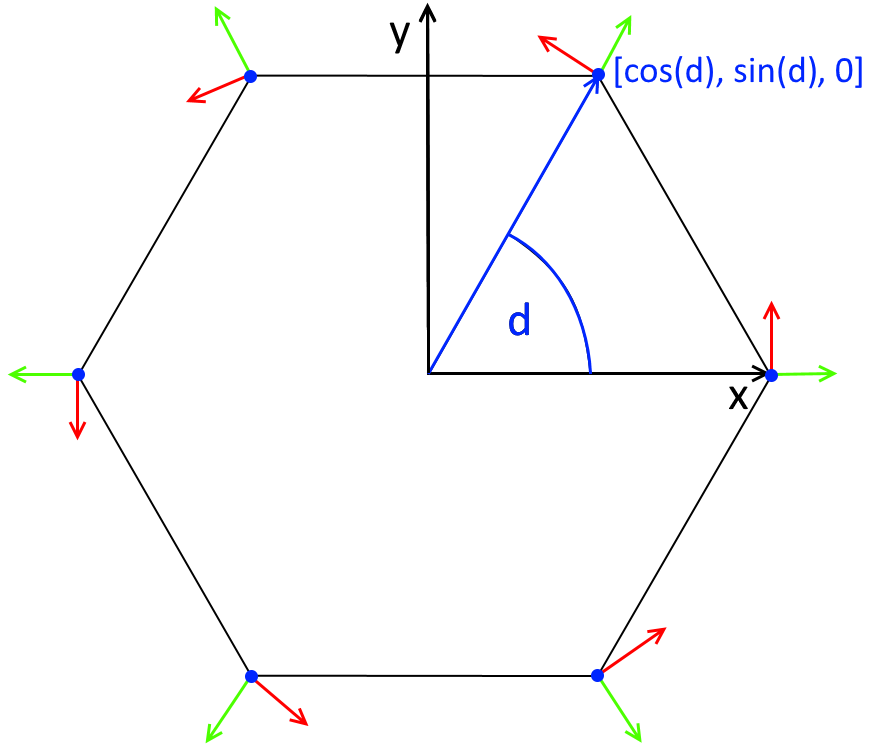
\includegraphics[height=0.25\textheight]{images/Ring6Sections.png}
	\caption{Beispiel für die Berechnung von Vertexpositionen auf einem Einheitskreis mit einer Genauigkeit von sechs Segmenten. $d = \frac{360\degree}{6} = 60 \degree$. Die blauen Punkte entsprechen den Positionen, die grünen Pfeile den Normalen und die roten Pfeile den Tangenten der Vertizes. Eigene Abbildung.}
	\label{fig:Ring6Sections}
\end{figure}
\paragraph{Verbindung der Kreise}
Um den Zylindermantel eines Astsegments zu bilden, werden zwei Kreise mithilfe der Start- und Enddaten des Objekts generiert. Jedes Segment eines Kreises wird mit dem entsprechenden Segment des anderen Kreises verbunden und bildet dadurch ein Zylindersegment. Ein Zylindersegment entspricht somit einem Rechteck. Da das Modell jedoch Dreiecksdaten benötigt, wird jedes Rechteck, wie in Abbildung \ref{subfig:Zylinder10SegmenteWireframe} dargestellt, aus zwei Dreiecken gebildet. \cite{ModelingByNumbersZylindersA:13}
\begin{figure} [hbtp]
\centering
\begin{subfigure}[t]{.4\textwidth}
	\centering
	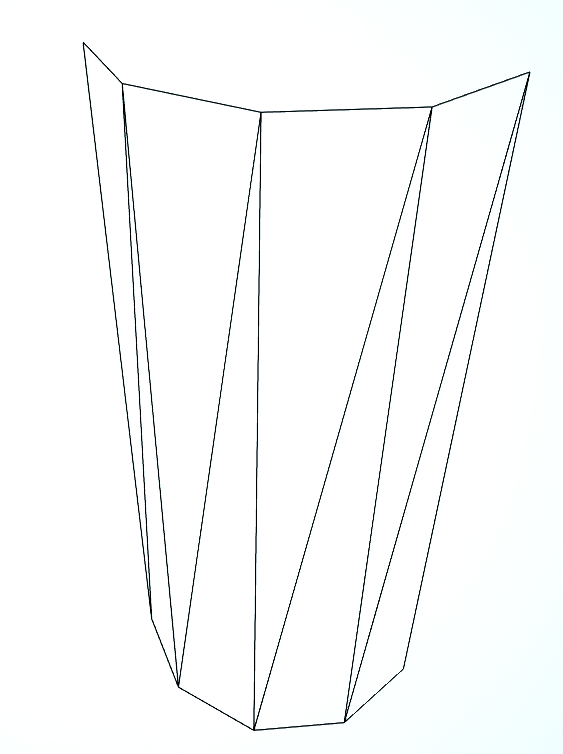
\includegraphics[height=.75\linewidth]{images/Zylinder10SegmenteWireframe.png}
	\caption{Darstellung der Dreiecke, welche bei der Verbindung der Kreise entstehen.}
	\label{subfig:Zylinder10SegmenteWireframe}
\end{subfigure}
\hspace{.1\textwidth}
\begin{subfigure}[t]{.4\textwidth}
	\centering
	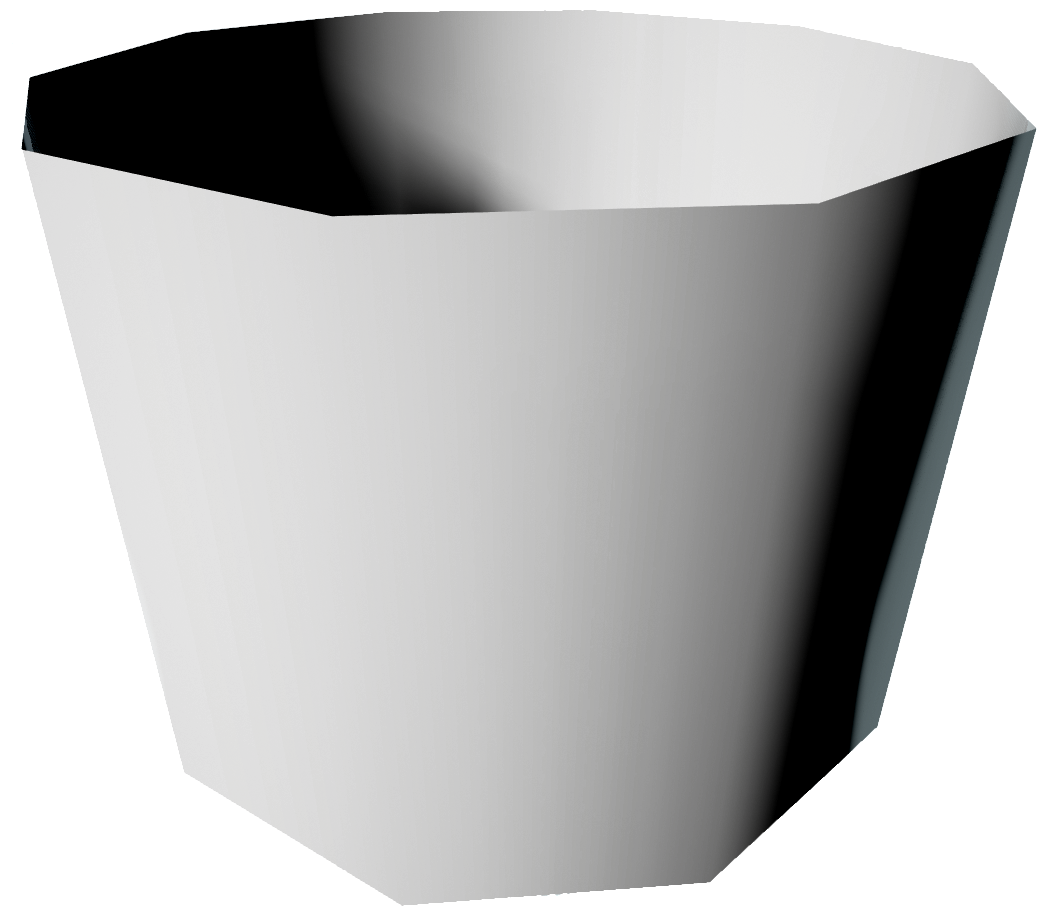
\includegraphics[height=.75\linewidth]{images/Zylinder10SegmenteOpaque.png}
	\caption{Gefärbte Dreiecke mit Beleuchtungsberechnung.}
	\label{subfig:Zylinder10SegmenteOpaque}
\end{subfigure}
\caption{Verbindung zweier Kreise zu einem Zylindermantel. Eigene Abbildungen.}
\label{fig:Zylinder10Segmente}
\end{figure}

Wird jedes Astsegment durch die Verbindung von genau zwei Kreisen dargestellt, führt dies zu der Generierung redundanter Vertexdaten. Die Enddaten eines Astsegments und die Startdaten seines Nachfolgers entsprechen einander, da die daraus generierten Kreis-Vertizes genau aufeinander liegen. Anstatt nun vier Kreise für die Generierung zweier Zylinder zu verwenden, können die Vertizes des verbindenden Kreises wiederverwendet werden -- es genügen drei Kreise für die Generierung zweier Zylinder.

Die Verbindung der Modelldaten kann für alle Astsegmente durchgeführt werden, deren Nachfolger dieselbe Zweigtiefe besitzen und somit eine Folge von zusammenhängenden Zylindermodellen bilden. Für einen Nachfolger mit einer sich unterscheidenden Zweigtiefe wird eine neue Folge von zusammenhängenden Zylindermodellen begonnen. \cite{ModelingByNumbersZylindersA:13}

Ein Beispiel für die Generierung zweier Zylinder mithilfe von drei Kreisen wird in Abbildung \ref{subfig:MultiZylinder10SegmenteWireframe} dargestellt.

\begin{figure} [hbtp]
	\centering
	\begin{subfigure}[t]{.4\textwidth}
		\centering
		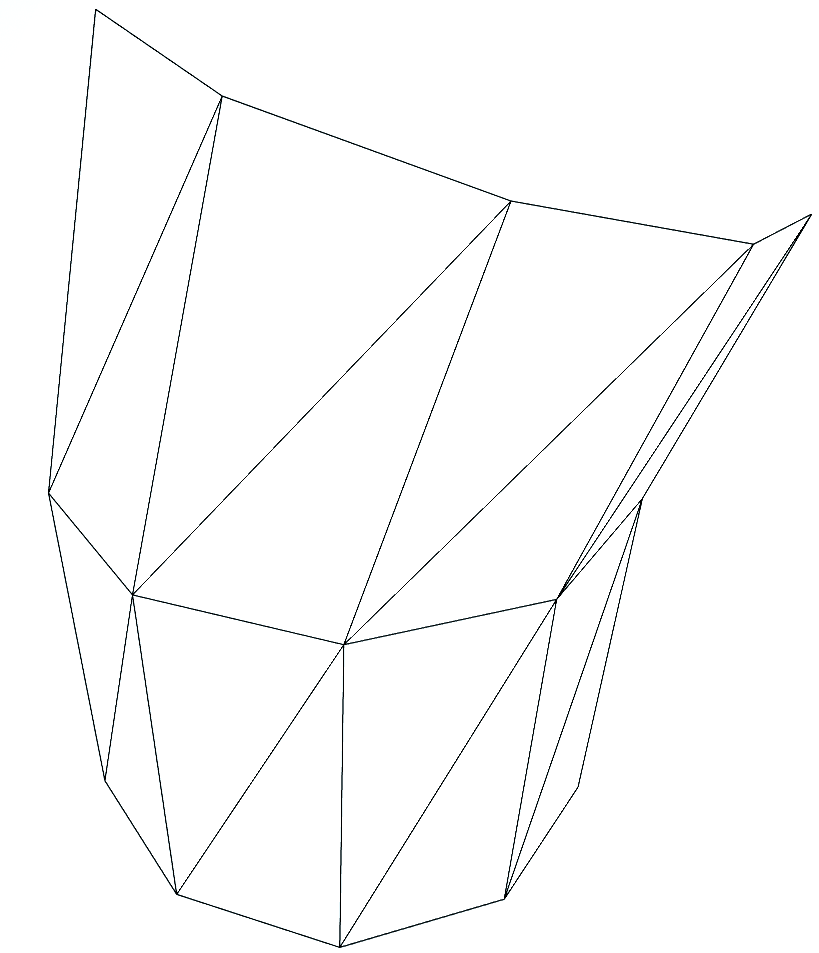
\includegraphics[height=\linewidth]{images/MultiZylinder10SegmenteWireframe.png}
		\caption{Darstellung der Dreiecke, welche bei der Verbindung der Kreise entstehen.}
		\label{subfig:MultiZylinder10SegmenteWireframe}
	\end{subfigure}
	\hspace{.1\textwidth}
	\begin{subfigure}[t]{.4\textwidth}
		\centering
		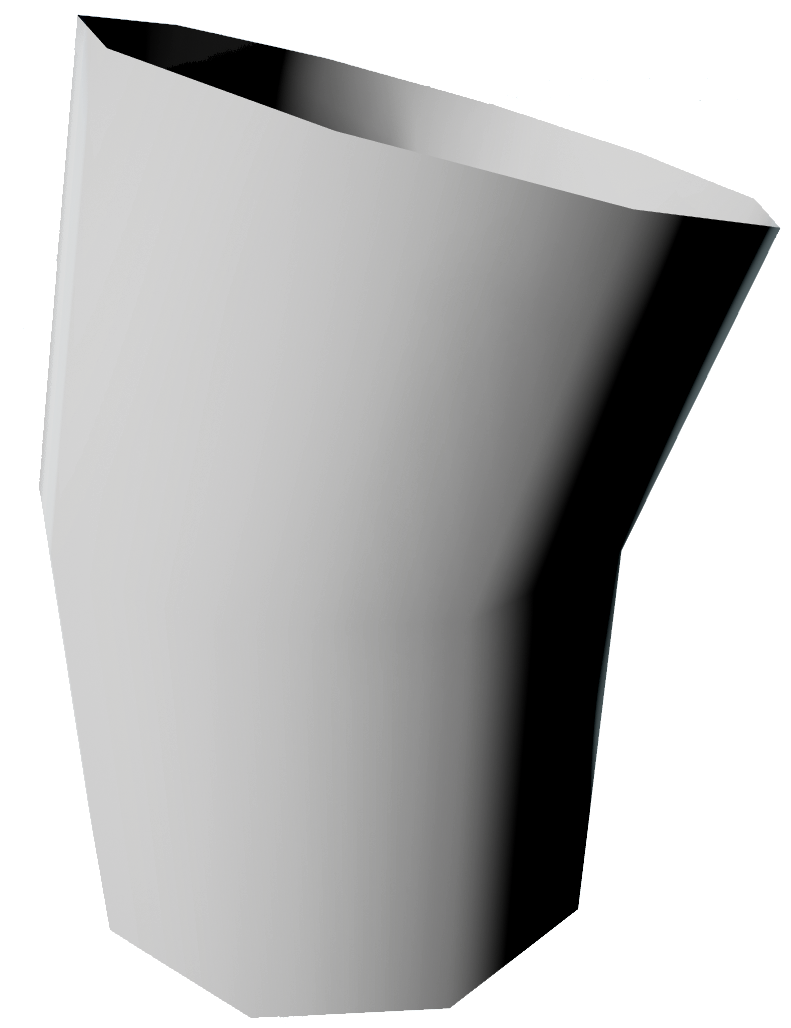
\includegraphics[height=\linewidth]{images/MultiZylinder10SegmenteOpaque.png}
		\caption{Gefärbte Dreiecke mit Beleuchtungsberechnung.}
		\label{subfig:MultiZylinder10SegmenteOpaque}
	\end{subfigure}
	\caption{Verbindung dreier Kreise zu einer Folge zusammenhängender Zylindermodelle. Eigene Abbildungen.}
	\label{fig:MultiZylinder10Segmente}
\end{figure}





\chapter{Ergebnisse}
In diesem Kapitel werden die Ergebnisse vorgestellt, die mithilfe der Implementierungen von L-Systemen und dem Space-Colonization Algorithmus produziert wurden. Es bietet sich an in vielen Fällen biologisch motivierte Begriffe zu verwenden -- beispielsweise Kanten als Äste oder Zweige zu bezeichnen -- um eine Verbindung zwischen visueller Repräsentation und graphentheoretischem Hintergrund zu schaffen.

\section{L-System-Actor}
L-Systeme ermöglichen es mithilfe bestimmter Produktionsregeln realitätsnahe Baumstrukturen zu generieren. Im Folgenden werden verschiedene natürliche Wachstumsarten mithilfe der L-System Implementierung nachgeahmt und visualisiert.
\subsection{Monopodiales Wachstum}
Ein biologischer Baum mit monopodialem Wachstumsverhalten bildet einen Hauptstamm, der stets weiterwächst, mit davon abzweigenden Nebenästen. \cite[S.14]{Deussen:05} Ein Beispiel für ein solches Wachstum ist das folgende L-System:

\begin{equation}
\begin{array}{llll}
\omega & : F(s)A(100) \\
p_1 & : A(l) &\rightarrow& F(l)\text{ }[\&(a1)\text{ }B(l)]\text{ }/(d1)\text{ }A(l*r1) \\
p_2 &  : B(l) &\rightarrow& F(l)\text{ }[-(a2)\text{ }B(l*r2)]\text{ }/(d2)\text{ }B(l*r2)
\end{array}
\label{eq:ProdMonopodial}
\end{equation} 
\cite[S.56]{ABOP:04}

Die Produktionsregel $p_1$ produziert den Hauptstamm, welcher in jeder Ableitung verlängert wird und einen Nebenast produziert, der anhand von $p_2$ ebenfalls entlang einer Hauptachse weiterwächst und weitere Nebenäste produziert. $a_1$ und $a_2$ entsprechen den Abzweigungswinkeln neuer Äste von der Hauptachse, während die Winkel $d_1$ und $d_2$ die Rotation um die Hauptachse beschreiben, bevor ein neuer Nebenast produziert wird. $r_1$ und $r_2$ entsprechen Faktoren, welche das Wachstum eines Astes pro Ableitung verkürzen, falls der Wert unter $1$ liegt und verlängern, falls der Wert über $1$ liegt. Die Variable $s$ beschreibt die Länge des Stammes, bevor das Wachstum beginnt. \cite[S.57]{ABOP:04}

Abbildung \ref{fig:LS_Monopodial} zeigt Beispiele für monopodiale Baumstrukturen, Tabelle \ref{tab:LS_Monopodial} die verwendeten Konstantenwerte. Es findet kein Einfluss durch Tropismus statt.
\begin{center}
	\begin{tabulary}{\textwidth}{|C|C|C|C|C|C|C|C|C|}
		\hline 
		Abbildung & $n$ & $a_1$ & $a_2$ & $r_1$ & $r_2$ & $d_1$ & $d_2$ & $s$ \\ 
		\hline 
		a & 11 & 45.0 & 35.0 & 1.05 & 0.9 & 137.5 & 70.0 & 100.0 \\ 
		\hline 
		b & 11 & 60.0 & 20.0 & 1.05 & 0.9 & 137.5 & 70.0 & 100.0 \\ 
		\hline 
		c & 11 & 45.0 & 35.0 & 0.95 & 0.9 & 137.5 & 70.0 & 350.0 \\ 
		\hline 
		d & 11 & 77.0 & -37.0 & 1.05 & 0.85 & 137.5 & -70.0 & 200.0 \\ 
		\hline 
	\end{tabulary} 
	\captionof{table}{Konstantenwerte der in Abbildung \ref{fig:LS_Monopodial} dargestellten monopodialen Baumstrukturen.} 
	\label{tab:LS_Monopodial}
\end{center}


\begin{figure} [hbtp]
	\centering
	\begin{subfigure}[t]{.45\textwidth}
		\centering
		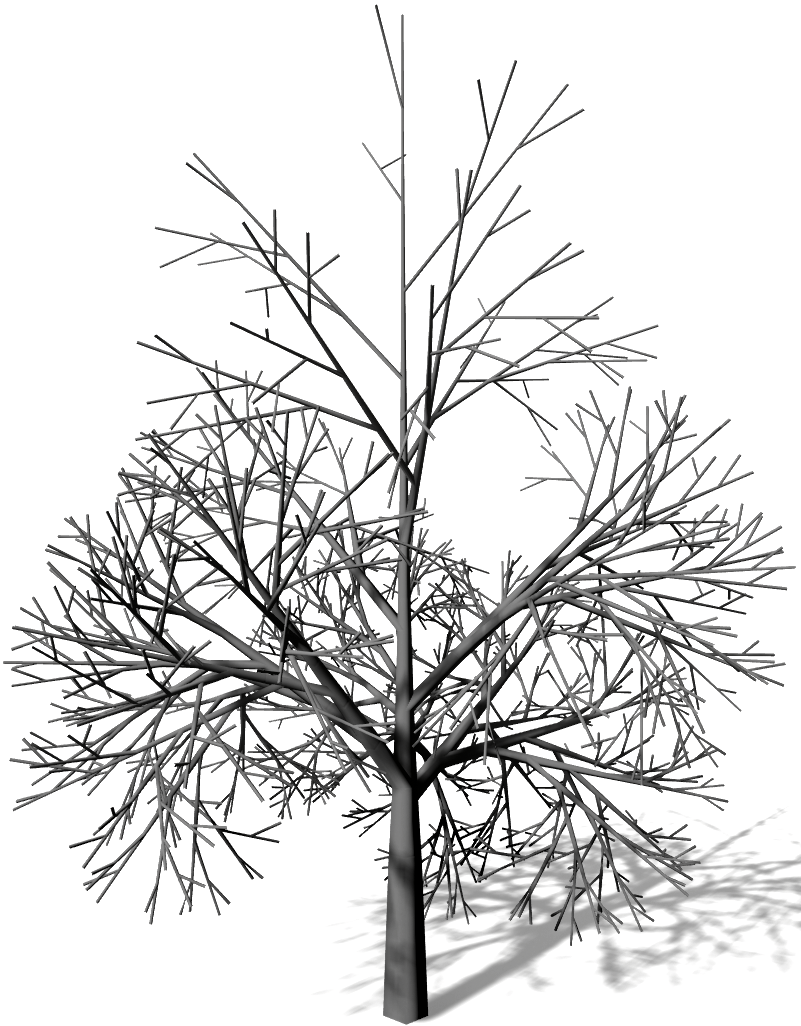
\includegraphics[height=.21\textheight]{images/LS_Monopodial_1.png}
		\caption{}
		\label{subfig:LS_Monopodial_1}
	\end{subfigure}
	\begin{subfigure}[t]{.45\textwidth}
		\centering
		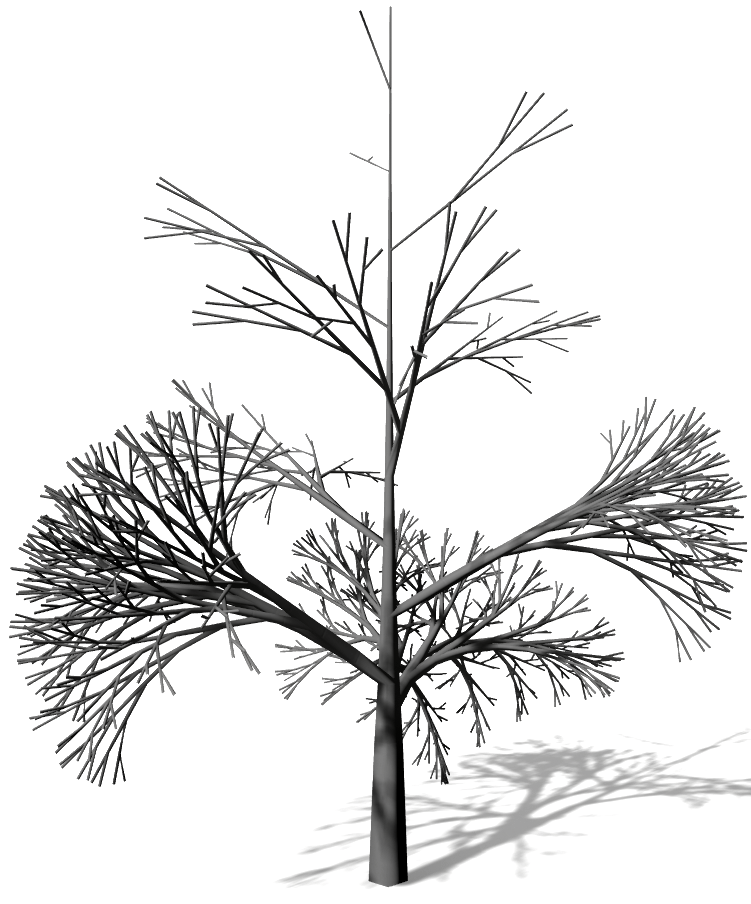
\includegraphics[height=.21\textheight]{images/LS_Monopodial_2.png}
		\caption{}
		\label{subfig:LS_Monopodial_2}
	\end{subfigure}	
	\begin{subfigure}[t]{.45\textwidth}
		\centering
		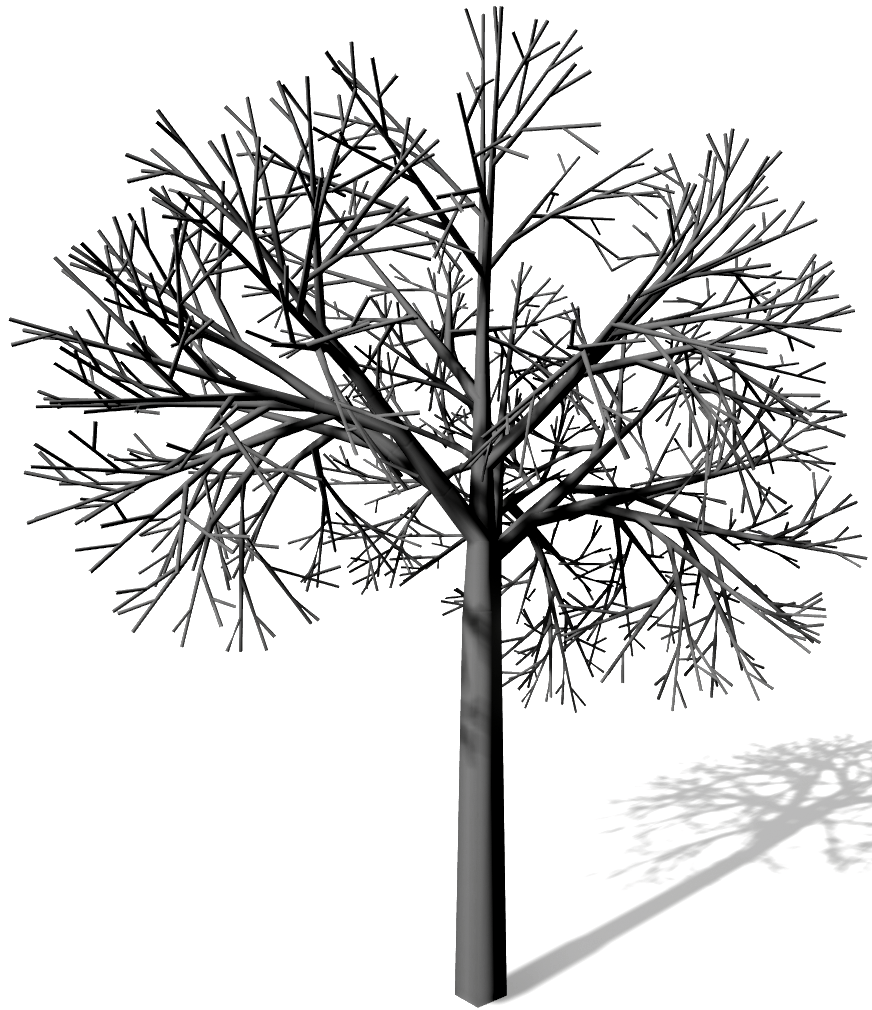
\includegraphics[height=.21\textheight]{images/LS_Monopodial_3.png}
		\caption{}
		\label{subfig:LS_Monopodial_3}
	\end{subfigure}
	\begin{subfigure}[t]{.45\textwidth}
		\centering
		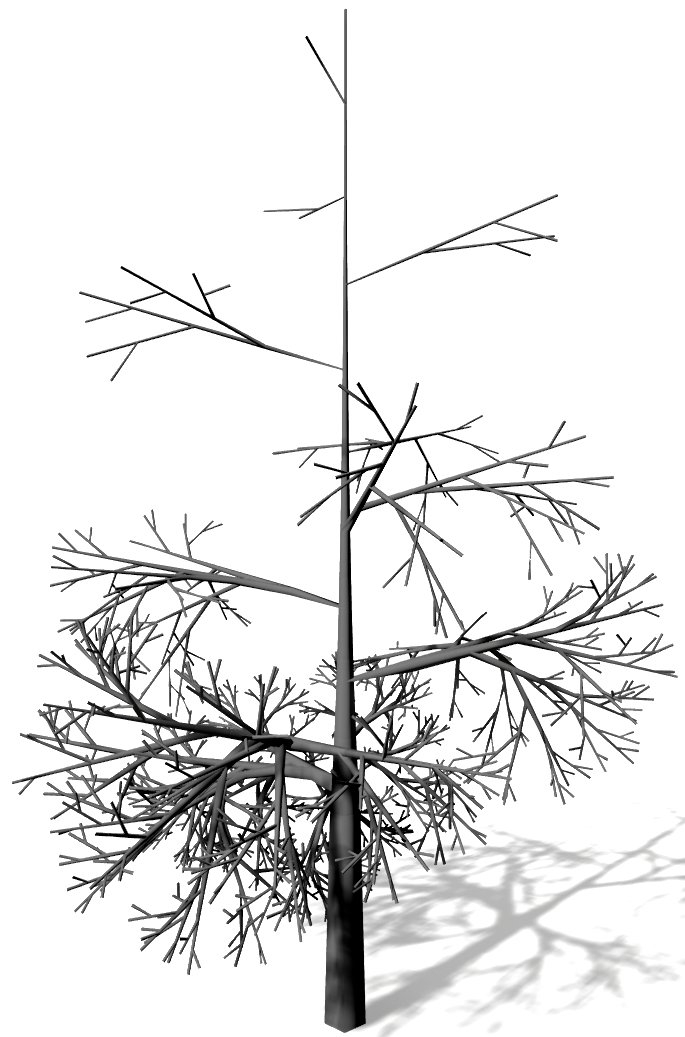
\includegraphics[height=.21\textheight]{images/LS_Monopodial_4.png}
		\caption{}
		\label{subfig:LS_Monopodial_4}
	\end{subfigure}
	\caption{Beispiele monopodialen Wachstums, entspricht der n-fachen Ableitung des Axioms anhand der Produktionsregeln aus Gleichung \ref{eq:ProdMonopodial}. Eigene Abbildungen.}
	\label{fig:LS_Monopodial}
\end{figure}

\subsection{Sympodiales Wachstum}
Beim sympodialen Wachstum bildet ein Ast mehrere Abzweigungen in einem Winkel ungleich $0\degree$. Der sich verzweigende Ast wächst daraufhin nicht weiter. \cite[S.14]{Deussen:05} \cite[S.58]{ABOP:04} Das folgende L-System simuliert ein solches Wachstum:

\begin{equation}
\begin{array}{llll}
\omega & : F(100)A(150) \\
p_1 & : A(l) &\rightarrow& F(l)\text{ }[\&(a1)\text{ }B(l*r1)]\text{ }/(180)\text{ }[\&(a2)\text{ }B(l*r2)] \\
p_2 &  : B(l) &\rightarrow& F(l)\text{ }[+(a1)\text{ }/(d1)\text{ }B(l*r1)]\text{ }[-(a2)\text{ }\backslash(d2)\text{ }B(l*r2)]
\end{array}
\label{eq:ProdSympodial}
\end{equation} 
\cite[S.59]{ABOP:04}
Die Produktionsregel $p_1$ beschreibt die Bildung der ersten, sich gegenüberliegenden, Abzweigungen während $p_2$ das Wachstum der abzweigenden Äste beschreibt, welche sich ebenfalls zu zwei Nebenästen aufteilen. $a_1$ und $a_2$ entsprechen den Abzweigungswinkeln, $r_1$ und $r_2$ den Wachstumsfaktoren pro Ableitung der Nebenäste. $d_1$ und $d_2$ beschreiben die Rotation eines Nebenastes um seine eigene Achse, bevor die nächste Abzweigung entsteht.

Abbildung \ref{fig:LS_Sympodial} zeigt Beispiele für sympodiale Baumstrukturen, Tabelle \ref{tab:LS_Sympodial} die verwendeten Konstantenwerte. Es findet kein Einfluss durch Tropismus statt.

\begin{center}
	\begin{tabulary}{\textwidth}{|C|C|C|C|C|C|C|C|}
		\hline 
		Abbildung & $n$ & $a_1$ & $a_2$ & $r_1$ & $r_2$ & $d_1$ & $d_2$ \\ 
		\hline 
		a & 10 & 5.0 & 65.0 & 0.9 & 0.75 & 50.0 & 50.0 \\ 
		\hline 
		b & 10 & 20.0 & 50.0 & 0.9 & 0.75 & 50.0 & 50.0 \\ 
		\hline 
		c & 10 & 35.0 & 35.0 & 1.0 & 0.8 & 50.0 & 50.0 \\ 
		\hline 
		d & 10 & 30.0 & 40.0 & 0.95 & 0.9 & 110.0 & 110.0 \\ 
		\hline 
	\end{tabulary} 
	\captionof{table}{Konstantenwerte der in Abbildung \ref{fig:LS_Sympodial} dargestellten sympodialen Baumstrukturen.} 
	\label{tab:LS_Sympodial}
\end{center}

\begin{figure} [hbtp]
	\centering
	\begin{subfigure}[t]{.45\textwidth}
		\centering
		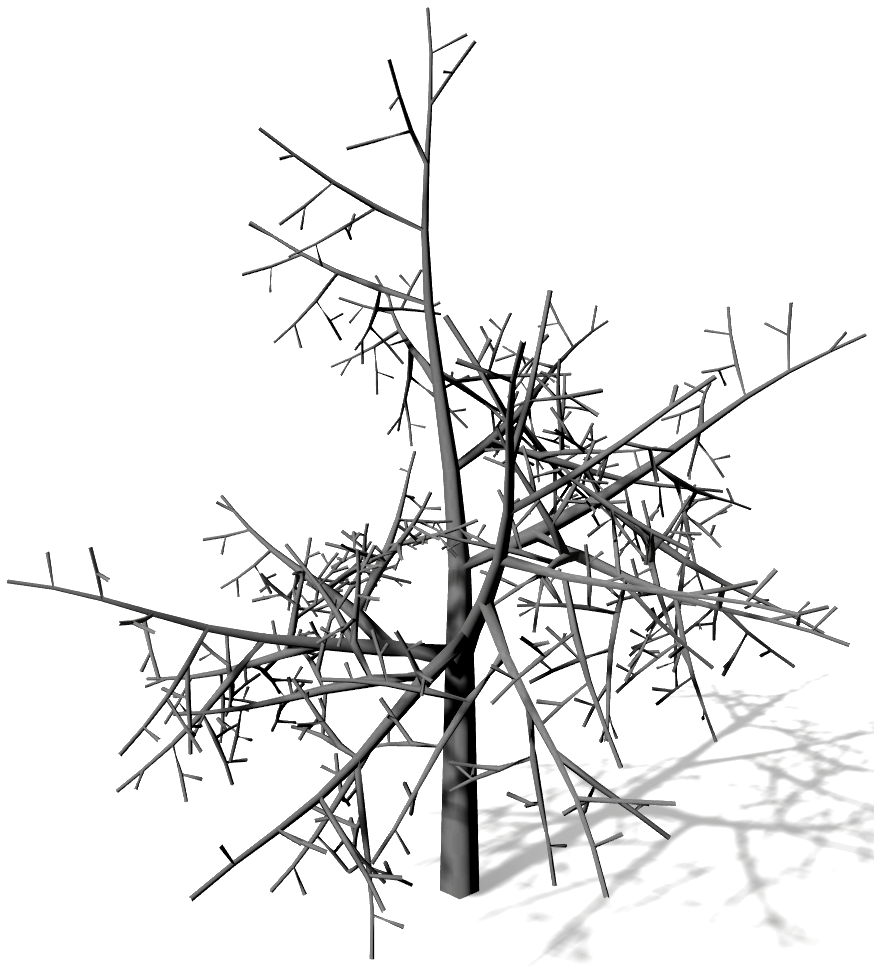
\includegraphics[height=.21\textheight]{images/LS_Sympodial_1.png}
		\caption{}
		\label{subfig:LS_Sympodial_1}
	\end{subfigure}
	\begin{subfigure}[t]{.45\textwidth}
		\centering
		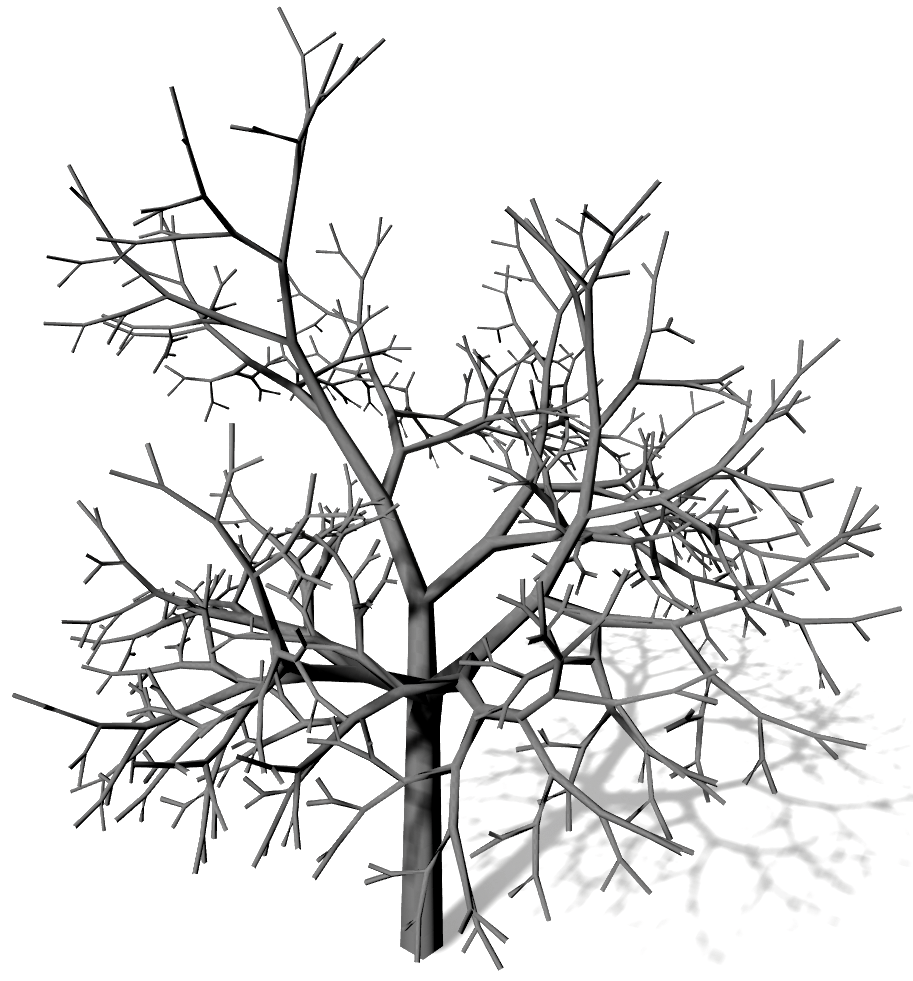
\includegraphics[height=.21\textheight]{images/LS_Sympodial_2.png}
		\caption{}
		\label{subfig:LS_Sympodial_2}
	\end{subfigure}	
	\begin{subfigure}[t]{.45\textwidth}
		\centering
		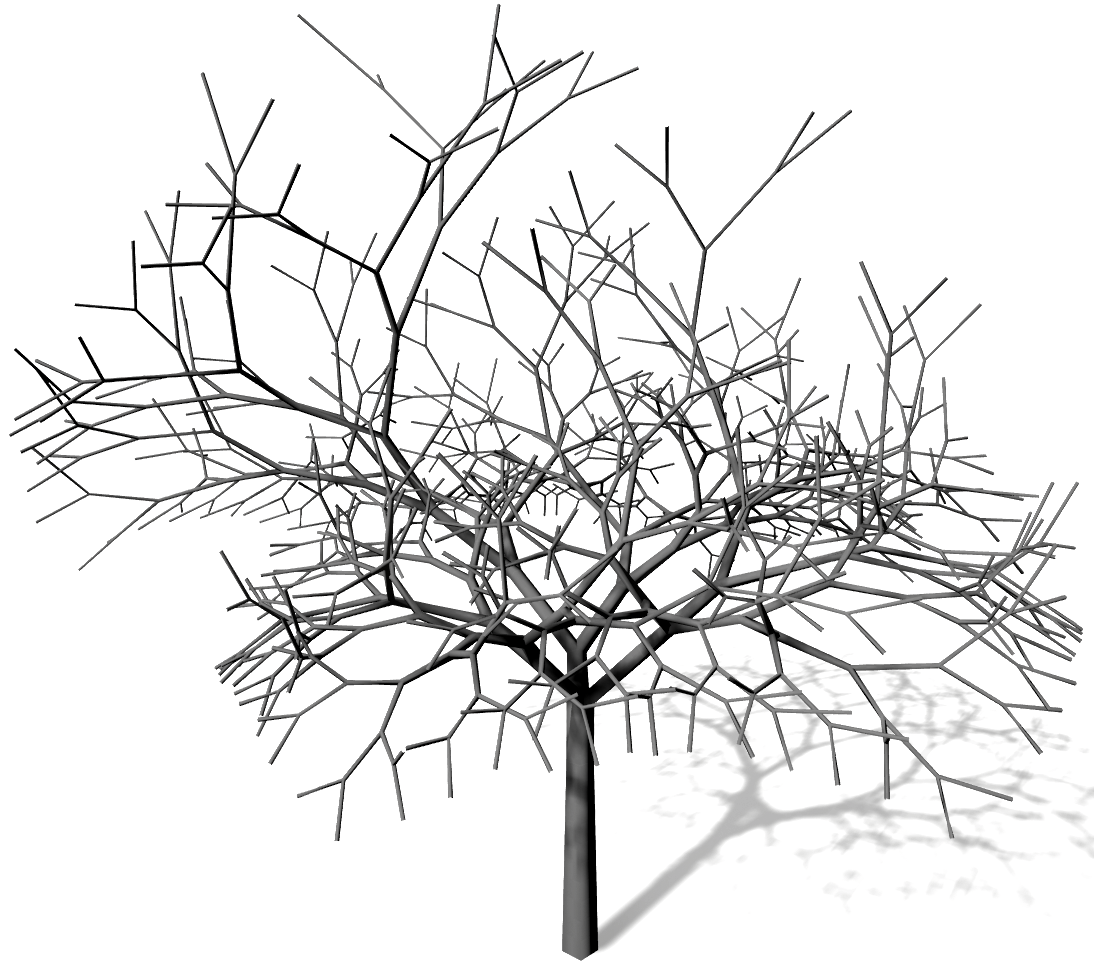
\includegraphics[height=.21\textheight]{images/LS_Sympodial_3.png}
		\caption{}
		\label{subfig:LS_Sympodial_3}
	\end{subfigure}
	\begin{subfigure}[t]{.45\textwidth}
		\centering
		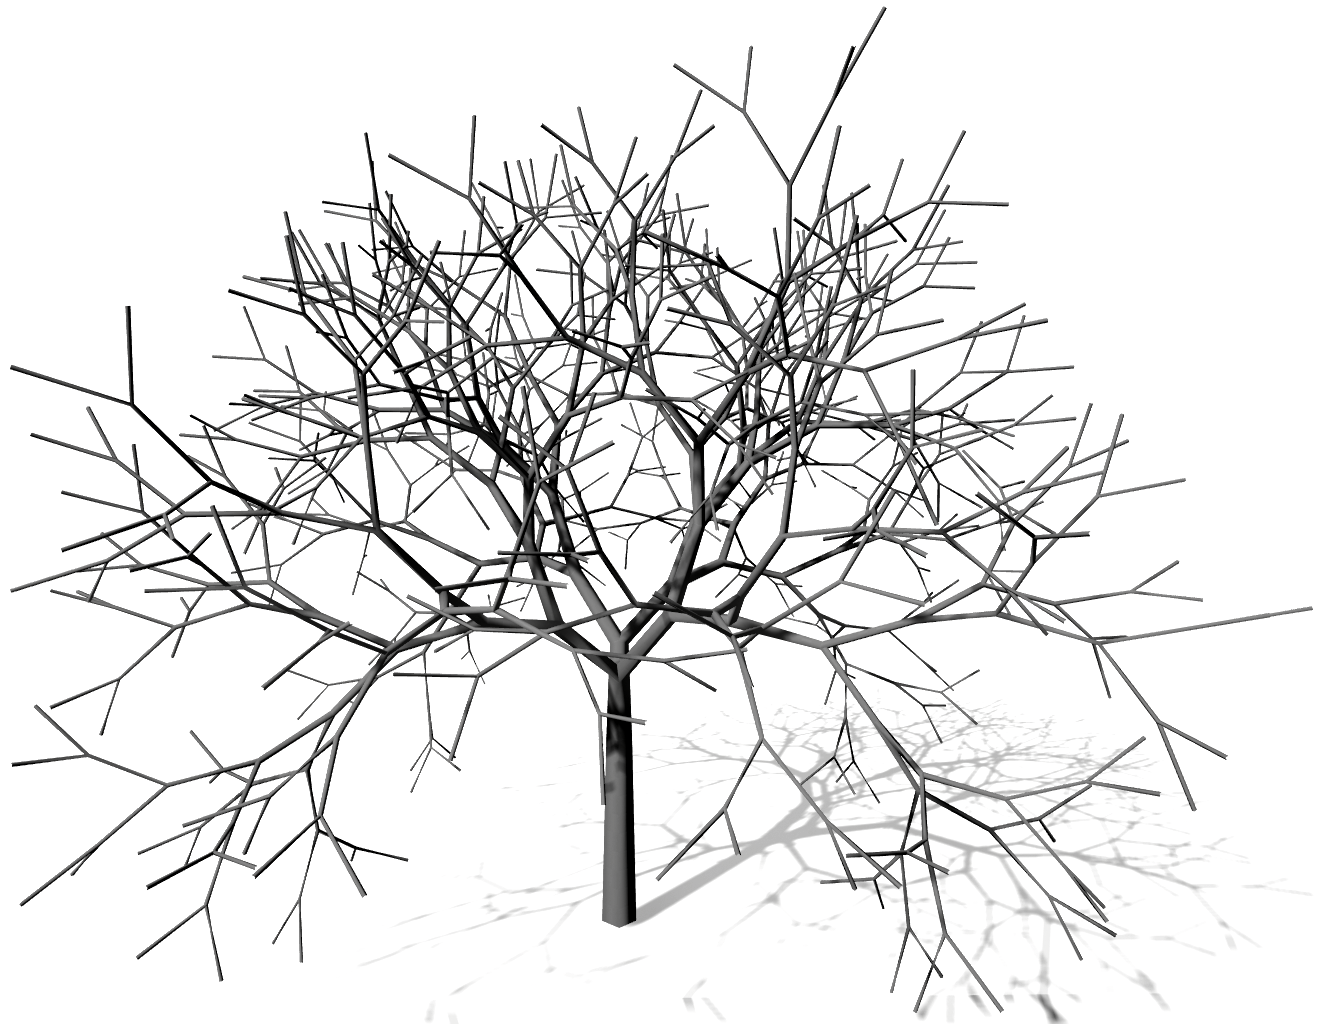
\includegraphics[height=.21\textheight]{images/LS_Sympodial_4.png}
		\caption{}
		\label{subfig:LS_Sympodial_4}
	\end{subfigure}
	\caption{Beispiele sympodialen Wachstums, entspricht der n-fachen Ableitung des Axioms anhand der Produktionsregeln aus Gleichung \ref{eq:ProdSympodial}. Eigene Abbildungen.}
	\label{fig:LS_Sympodial}
\end{figure}


\subsection{Ternäre Verzweigungen}

Eine andere Herangehensweise zur Bestimmung von L-Systemen für realistisch wirkende Baumstrukturen ist die Beschreibung von Selbstähnlichkeit, wie sie oft in der Natur zu finden ist. \cite[S.173]{ABOP:04} Das L-System aus Gleichung \ref{eq:ProdTernary} entspricht einem Wachstum, in welchem drei Abzweigungen mithilfe von Produktion $p_1$ auf dieselbe Art erstellt werden. In Produktion $p_2$ wird beschrieben wie Kanten aus vorhergehenden Ableitungen um einen Faktor $l_r$ verlängert werden. \cite[S.58]{ABOP:04}

\begin{equation}
\begin{array}{llll}
\omega & : /(45)A \\
p_1 & : A &\rightarrow& F(l_s)\text{ }[\&(a)\text{ }F(l_s)\text{ }A]\text{ }/(d1)\text{ }[\&(a)\text{ }F(l_s)\text{ }A]\text{ }/(d2)\text{ }[\&(a)\text{ }F(l_s)\text{ }A] \\
p_2 &  : F(l) &\rightarrow& F(l * l_r)
\end{array}
\label{eq:ProdTernary}
\end{equation} 
\cite[S.60]{ABOP:04}

$a$ entspricht dem Abzweigungswinkel von der Ursprungsachse, $d_1$ und $d_2$ der Rotation um die Achse, bevor eine neue Abzweigung produziert wird. $l_s$ ist die Anfangslänge der Kanten. \cite[S.58]{ABOP:04}

Abbildung \ref{fig:LS_Ternary} zeigt verschiedene ternär verzweigte Baumstrukturen, die auf den in Tabelle \ref{tab:LS_Ternary} gelisteten Konstantenwerten aufgebaut sind.

\begin{center}
	\begin{tabulary}{\textwidth}{|C|C|C|C|C|C|C|}
		\hline 
		Abbildung & $n$ & $a$ & $d_1$ & $d_2$ & $l_r$ & $l_s$ \\ 
		\hline 
		a & 6 & 19.0 & 95.0 & 132.0 & 1.1 & 50.0 \\ 
		\hline 
		b & 8 & 19.0 & 137.5 & 137.5 & 1.2 & 50.0 \\ 
		\hline 
		c & 8 & 27.0 & 77.0 & 77.0 & 1.3 & 50.0 \\ 
		\hline 
		d & 8 & 31.0 & 120.0 & 190.0 & 1.2 & 50.0 \\ 
		\hline 
	\end{tabulary} 
	\captionof{table}{Konstantenwerte der in Abbildung \ref{fig:LS_Ternary} dargestellten ternär verzweigten Baumstrukturen.} 
	\label{tab:LS_Ternary}
\end{center}

\begin{figure} [hbtp]
	\centering
	\begin{subfigure}[t]{.45\textwidth}
		\centering
		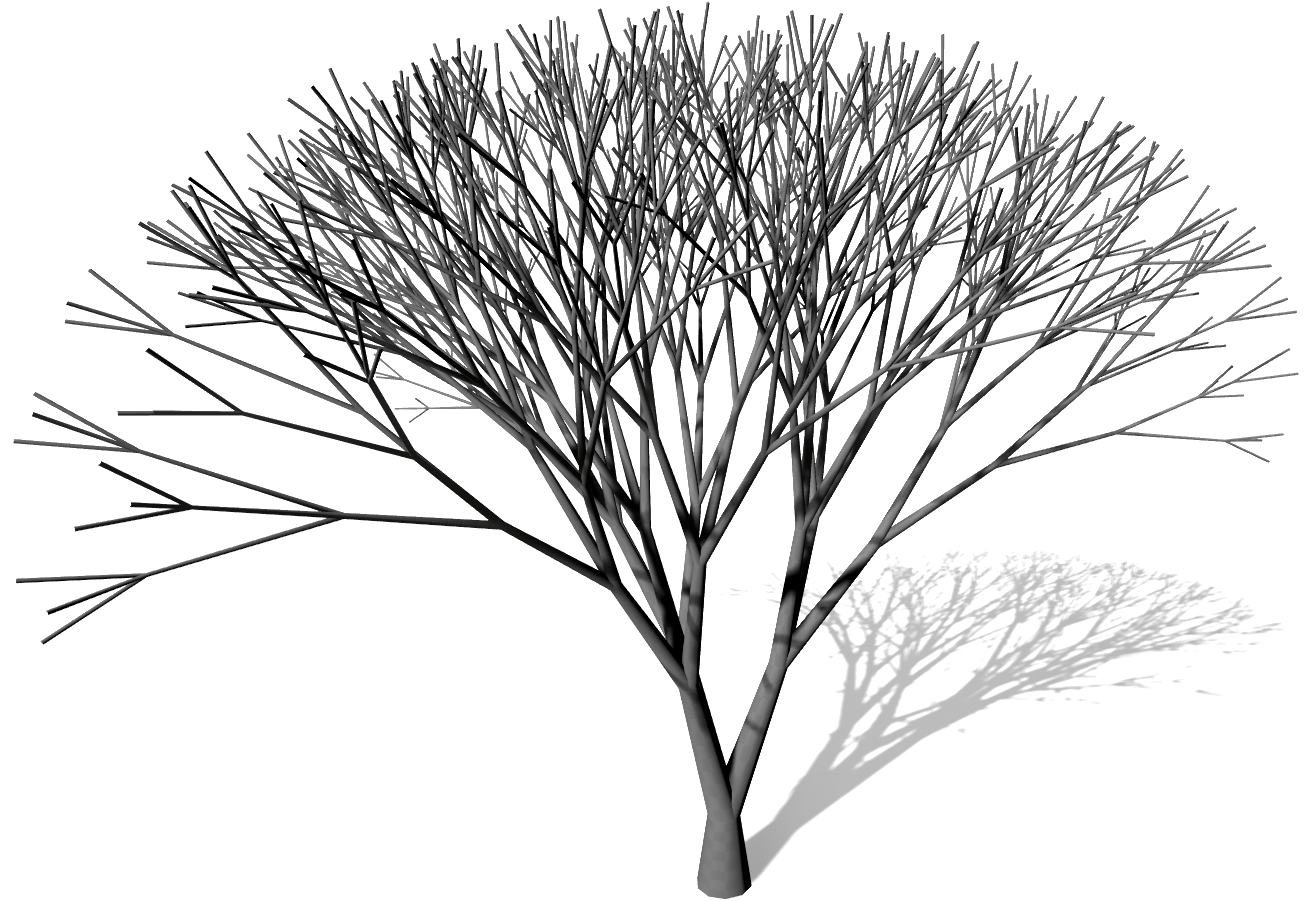
\includegraphics[width=\linewidth]{images/LS_Ternary_1.png}
		\caption{}
		\label{subfig:LS_Ternary_1}
	\end{subfigure}
	\begin{subfigure}[t]{.45\textwidth}
		\centering
		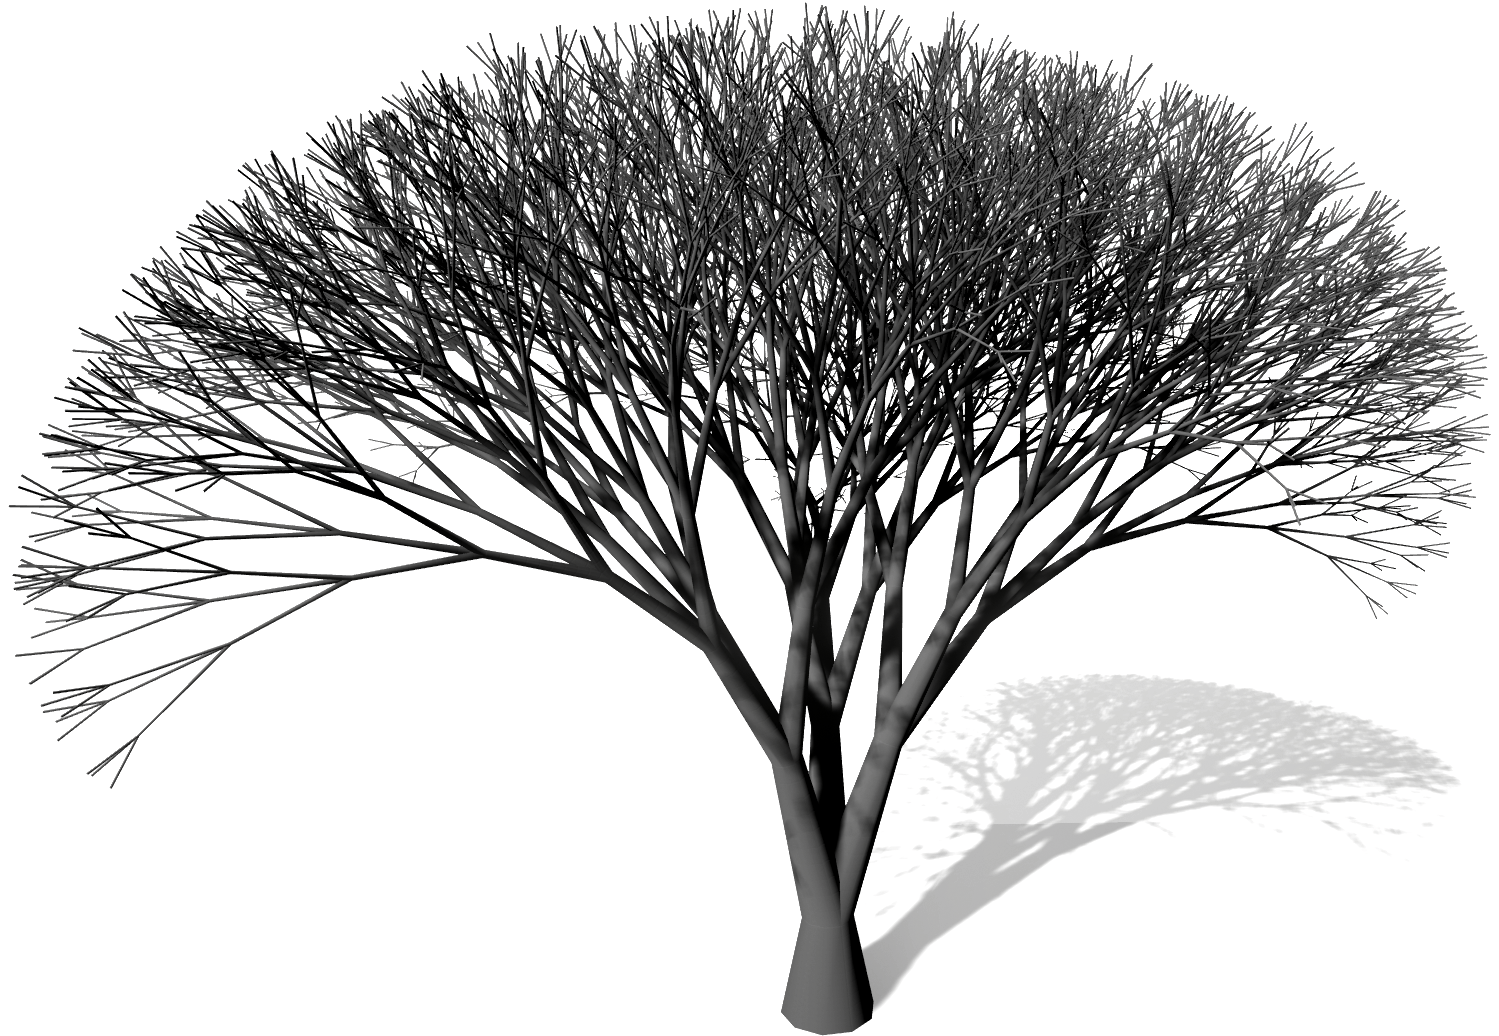
\includegraphics[width=\linewidth]{images/LS_Ternary_2.png}
		\caption{}
		\label{subfig:LS_Ternary_2}
	\end{subfigure}	
	\begin{subfigure}[t]{.45\textwidth}
		\centering
		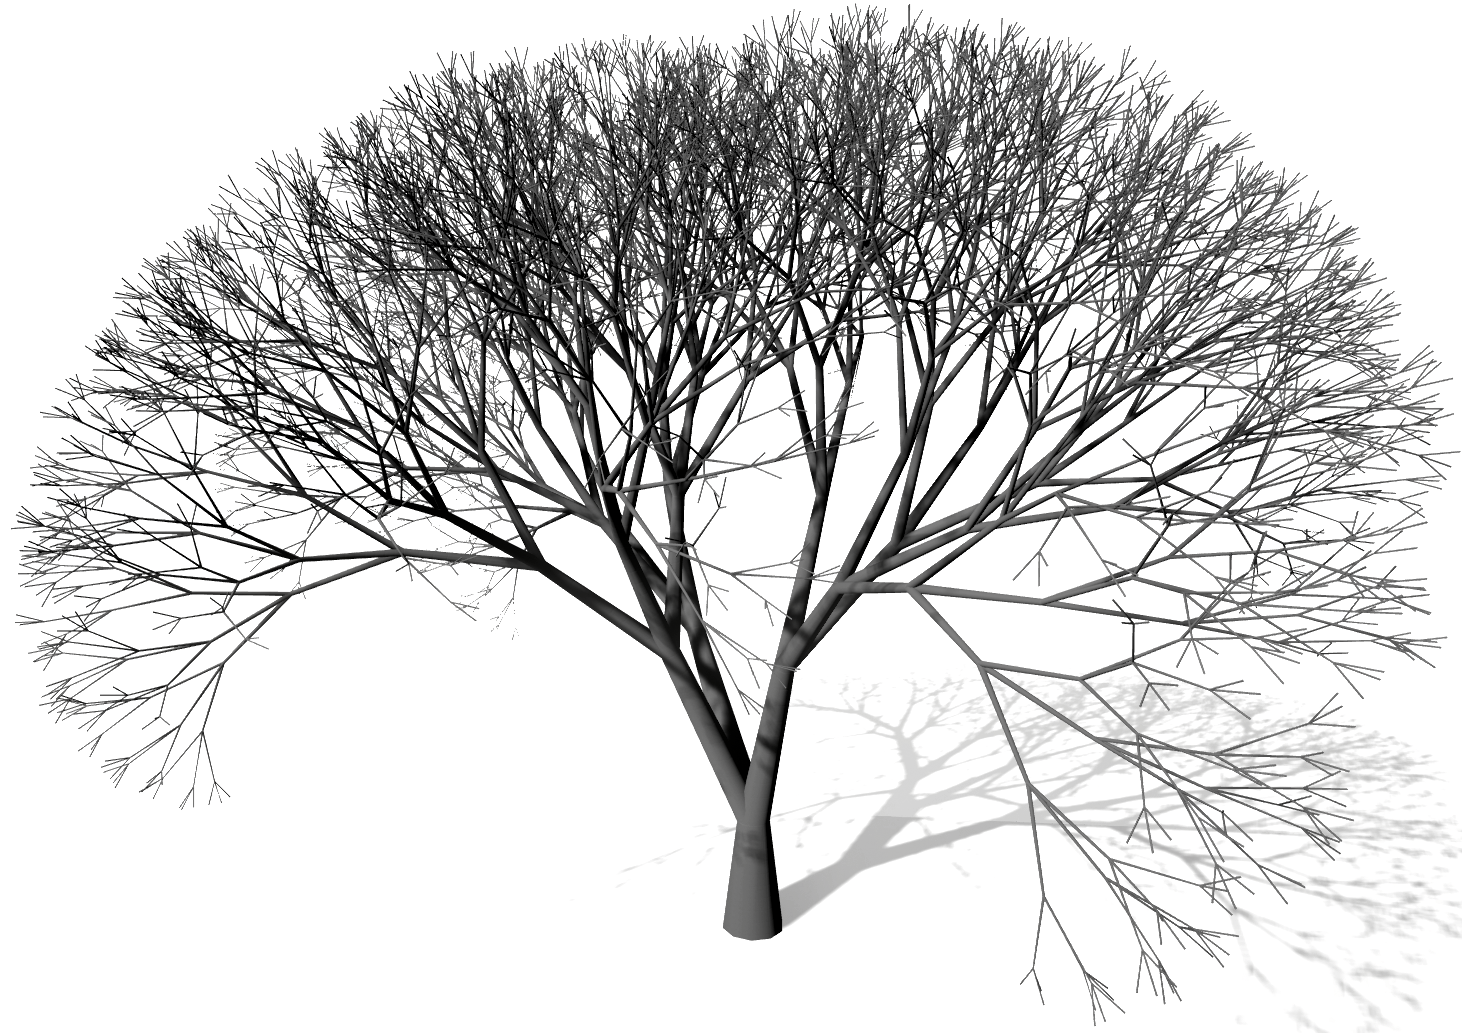
\includegraphics[width=\linewidth]{images/LS_Ternary_3.png}
		\caption{}
		\label{subfig:LS_Ternary_3}
	\end{subfigure}
	\begin{subfigure}[t]{.45\textwidth}
		\centering
		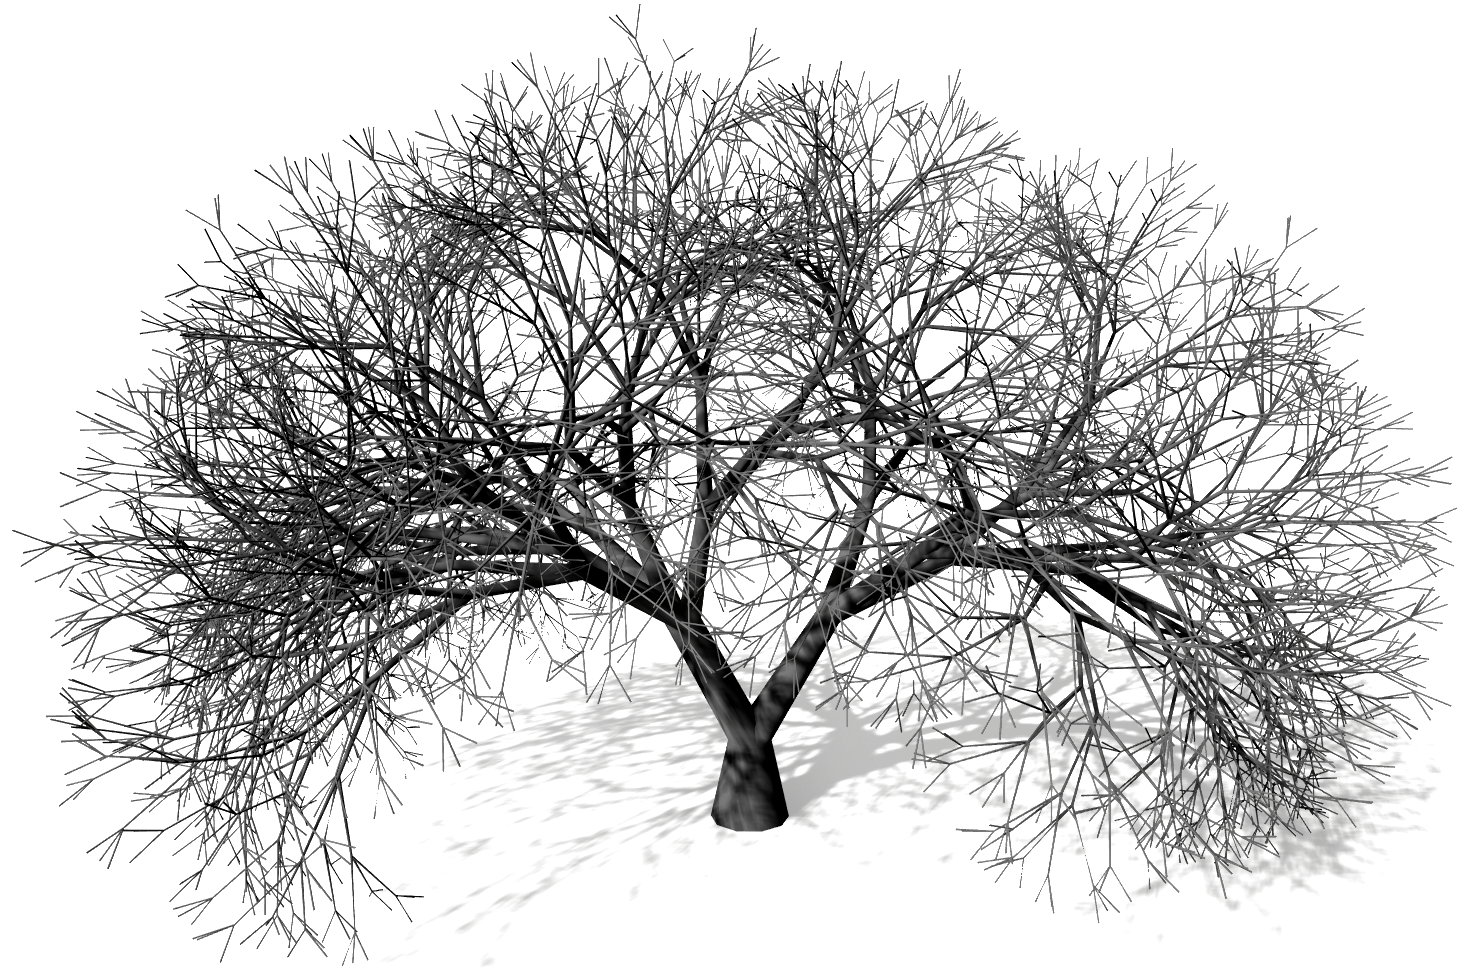
\includegraphics[width=\linewidth]{images/LS_Ternary_4.png}
		\caption{}
		\label{subfig:LS_Ternary_4}
	\end{subfigure}
	\caption{Beispiele ternären Wachstums, entspricht der n-fachen Ableitung des Axioms anhand der Produktionsregeln aus Gleichung \ref{eq:ProdTernary}. Eigene Abbildungen.}
	\label{fig:LS_Ternary}
\end{figure}


\subsection{Tropismus}

Der Einfluss von Tropismus führt, bei Eingabe derselben Werte bei den restlichen Parametern, zu visuell unterschiedlichen Ergebnissen. Dadurch können reale Einflüsse wie die Einwirkung von Wind, Sonne und Gravitation simuliert sowie die Wiederverwendbarkeit von L-System Definitionen erhöht werden. \cite[S.58]{ABOP:04}

Abbildung \ref{fig:LS_Ternary_Tropism} zeigt den Einfluss von Tropismus auf Baumstrukturen aus Abbildung \ref{fig:LS_Ternary}, welche ohne die Einwirkung von Tropismus produziert wurden.


\begin{figure} [hbtp]
	\centering
	\begin{subfigure}[t]{.45\textwidth}
		\centering
		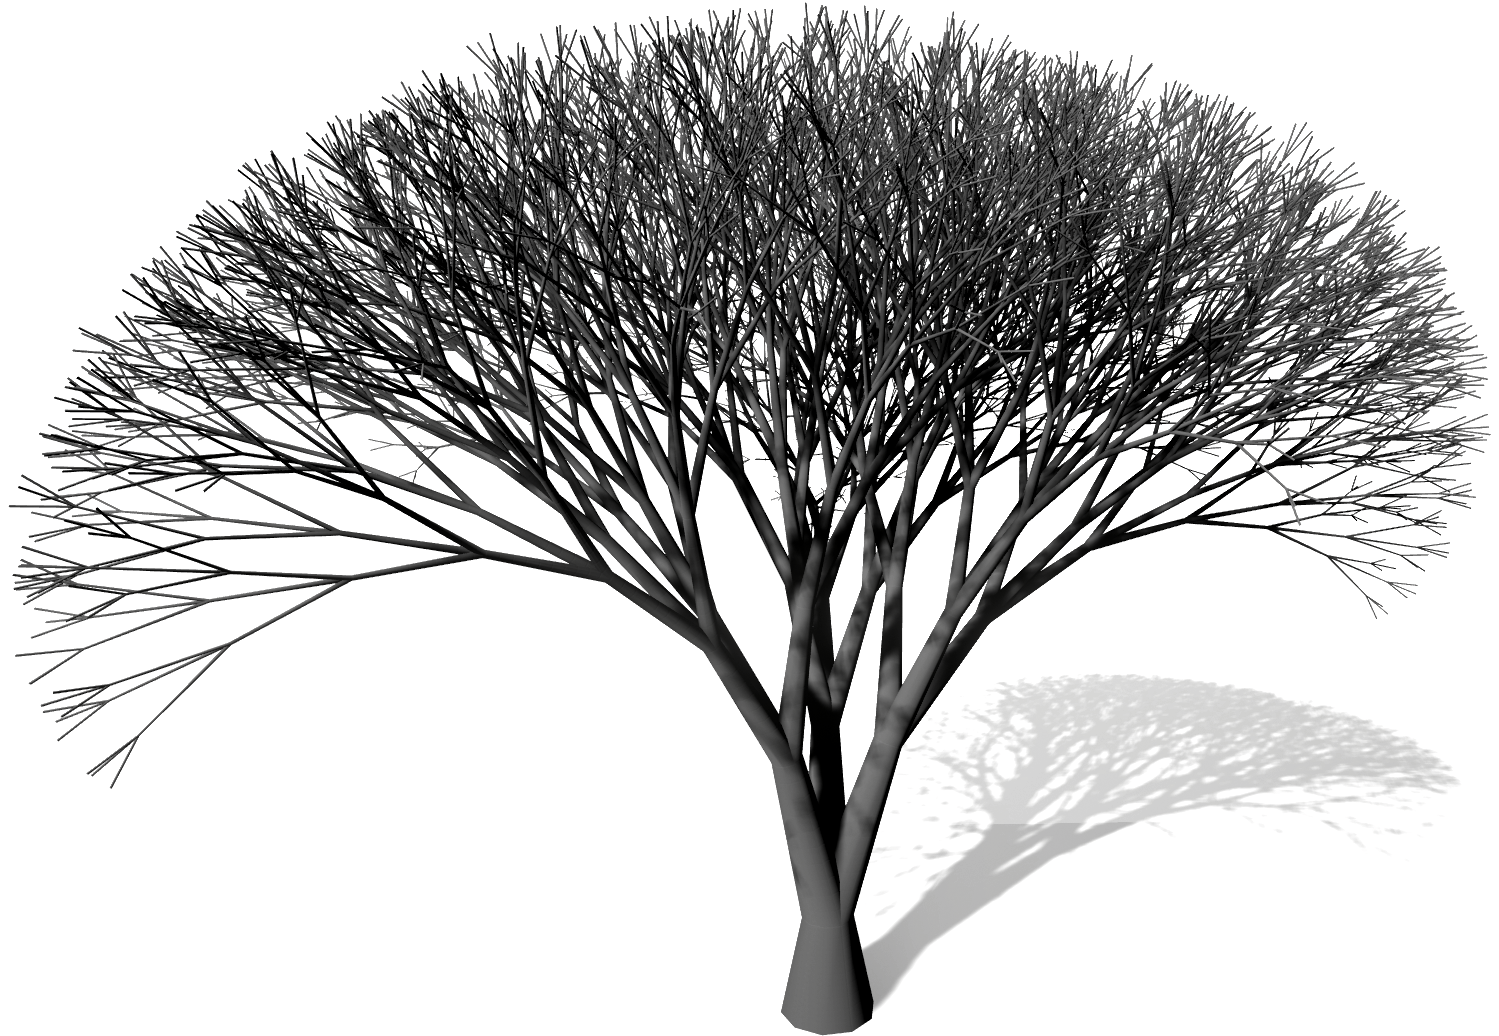
\includegraphics[width=\linewidth]{images/LS_Ternary_2.png}
		\caption{$\overrightarrow{T} = \overrightarrow{0}$, $e = 0$ \\ Entspricht Abbildung \ref{subfig:LS_Ternary_2}.}
		\label{subfig:LS_Ternary_2.2}
	\end{subfigure}
	\begin{subfigure}[t]{.45\textwidth}
		\centering
		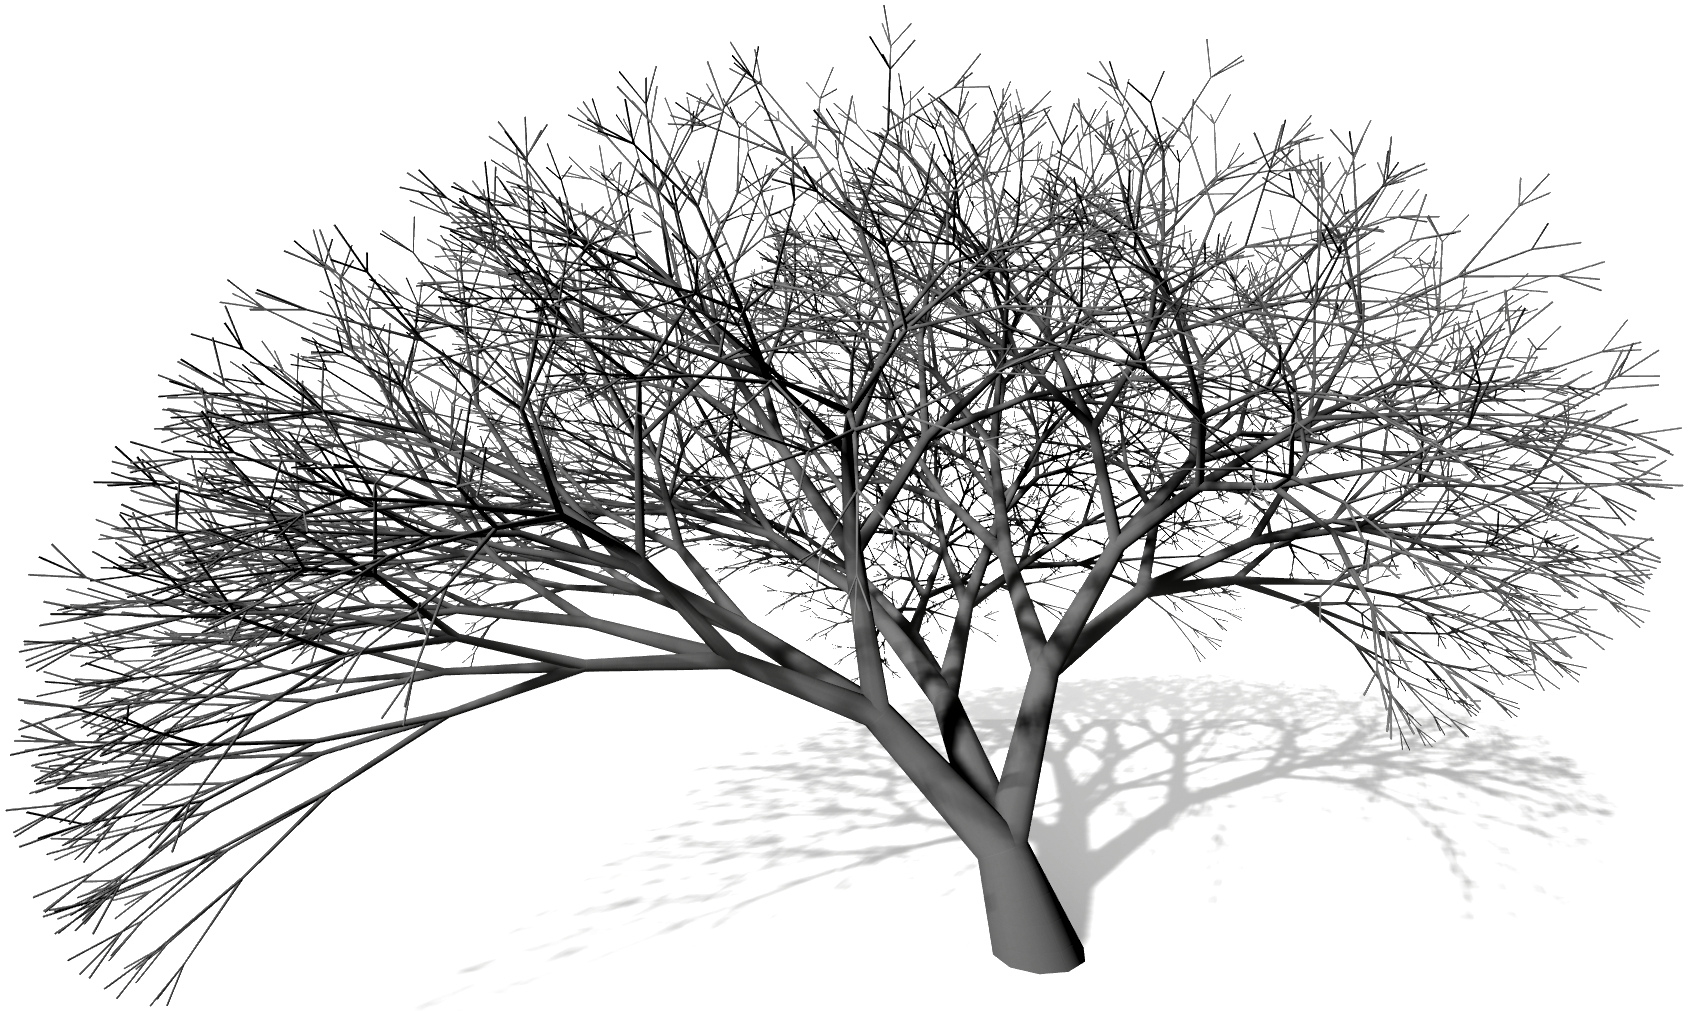
\includegraphics[width=\linewidth]{images/LS_Ternary_2_Tropism.png}
		\caption{$\overrightarrow{T} = \protect\begin{pmatrix}
			0 \\
			-0.5 \\
			-1
			\protect\end{pmatrix}$, $e = 0.5$}
		\label{subfig:LS_Ternary_2_Tropism}
	\end{subfigure}	
	\begin{subfigure}[t]{.45\textwidth}
		\centering
		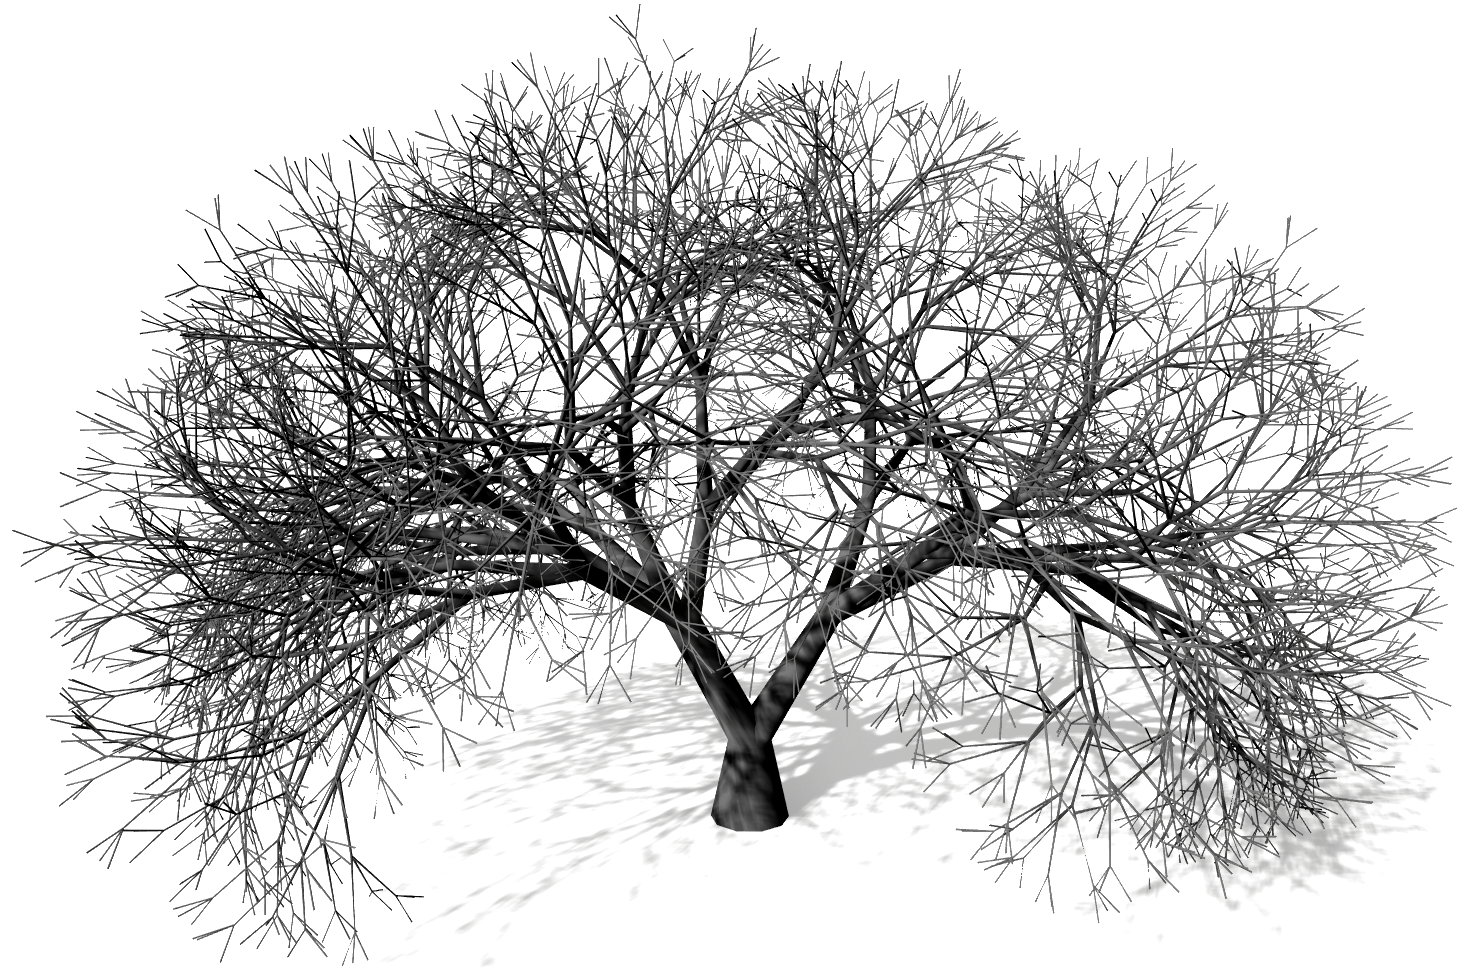
\includegraphics[width=\linewidth]{images/LS_Ternary_4.png}
		\caption{$\overrightarrow{T} = \overrightarrow{0}$, $e = 0$\\ Entspricht Abbildung \ref{subfig:LS_Ternary_4}.}
		\label{subfig:LS_Ternary_4.2}
	\end{subfigure}
	\begin{subfigure}[t]{.45\textwidth}
		\centering
		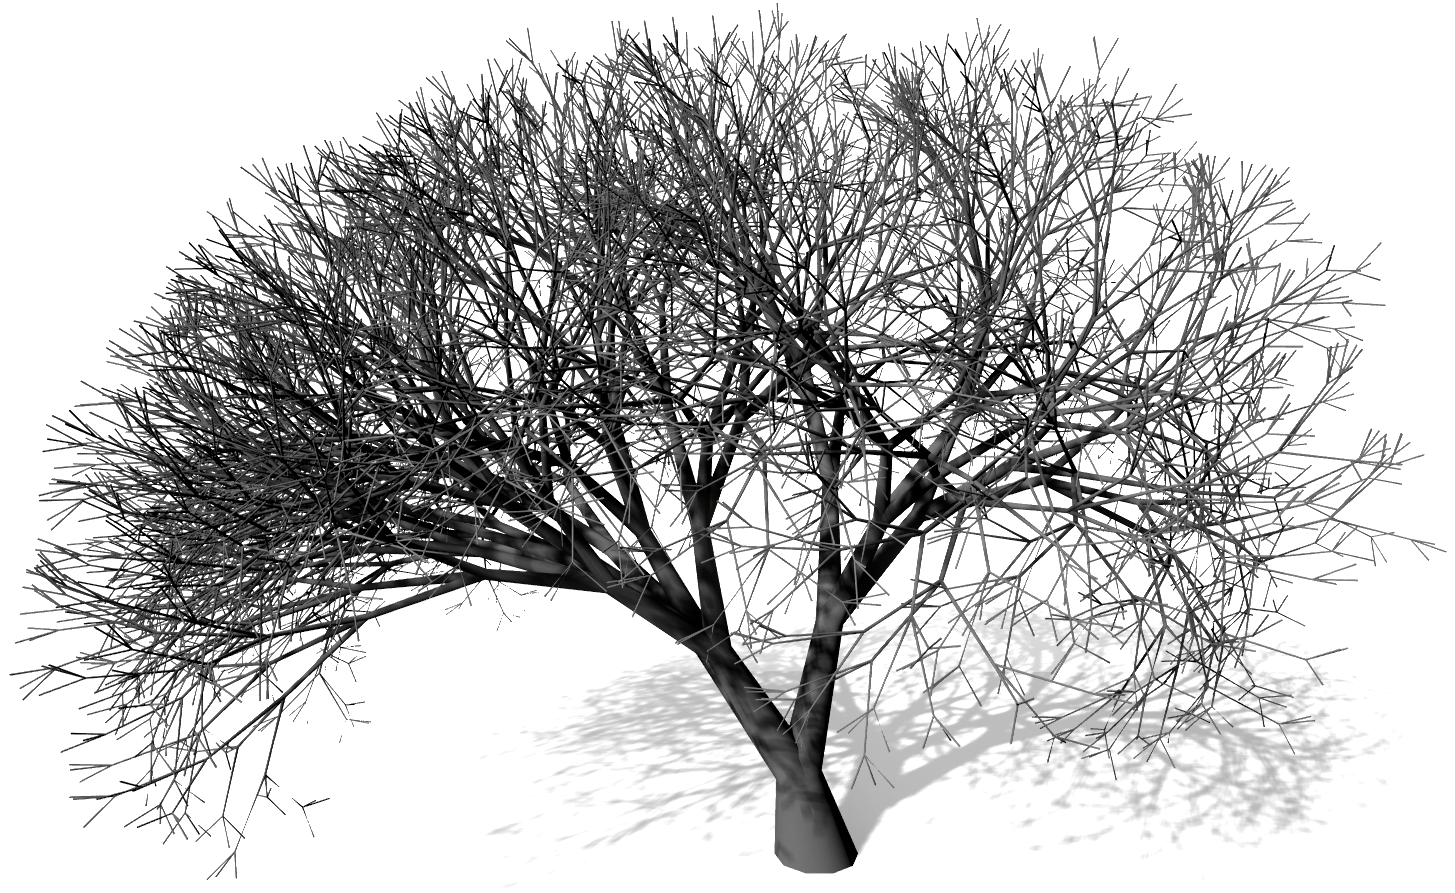
\includegraphics[width=\linewidth]{images/LS_Ternary_4_Tropism.png}
		\caption{$\overrightarrow{T} = \protect\begin{pmatrix}
			1 \\
			0 \\
			1
			\protect\end{pmatrix}$, $e = 0.3$}
		\label{subfig:LS_Ternary_4_Tropism}
	\end{subfigure}
	\caption{Beispiele ternären Wachstums mit und ohne Einfluss durch Tropismus. Entspricht der n-fachen Ableitung des Axioms anhand der Produktionsregeln aus Gleichung \ref{eq:ProdTernary}. Die linken und rechten Abbildungen unterscheiden sich jeweils im Tropismusvektor $\protect\overrightarrow{T}$ und im Biegsamkeitsfaktor $e$. Eigene Abbildungen.}
	\label{fig:LS_Ternary_Tropism}
\end{figure}

\section{Space-Colonization-Actor}

Die Space-Colonization Implementierung ermöglicht es durch die Angabe einiger weniger Parameter eine Vielzahl verschiedener Baumstrukturen zu generieren. \cite[S.3]{SpaceColonizationAlgorithm:07} Im Folgenden wird der Einfluss dieser Parameter auf die Ergebnisse untersucht. Es werden jeweils sich unterscheidende Parameterwerte angegeben.

\subsection{Einflussbereiche}

Die Verteilung und Anzahl der Einflusspunkte hat starke Auswirkungen auf die sich ergebende Baumstruktur. Je weniger Einflusspunkte existieren, desto größer ist die Wirkung jedes Punktes auf die Position der neuen Knotenpunkte und resultiert in einer spärlich bewachsenen Baumkrone mit kantigen, ungleichmäßig verteilten Ästen. Wird die Anzahl der Einflusspunkte erhöht, entsteht eine dicht bewachsene Baumkrone mit leicht kurvenförmigen, gleichmäßig verteilten Ästen. \cite[S.3]{SpaceColonizationAlgorithm:07}

Weiterhin passt sich die generierte Baumstruktur dem Bereich an, in welchem die Einflusspunkte generiert werden. Es können entweder einzelne Bereichprimitive, wie eine Kugel- oder Zylinderform, oder mehrere miteinander verknüpfte Einflussbereiche verwendet werden. \cite[S.4]{SpaceColonizationAlgorithm:07}

\begin{figure} [hbtp]
	\centering
	\begin{subfigure}[t]{.45\textwidth}
		\centering
		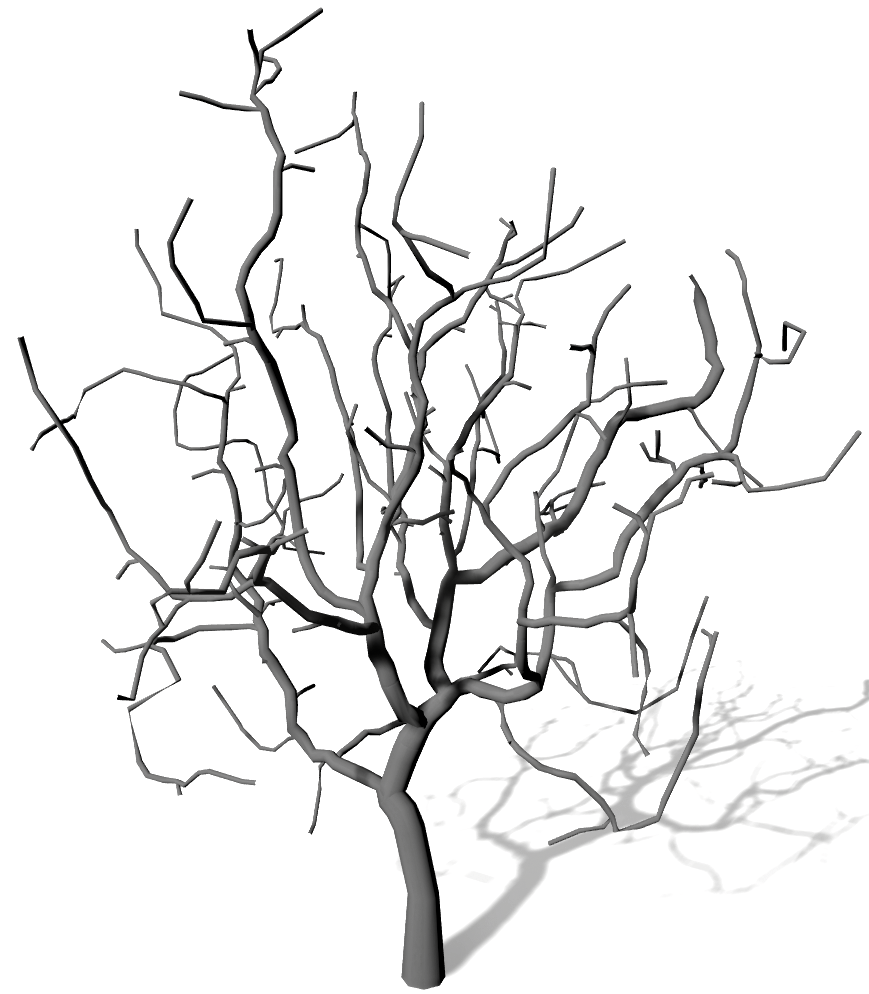
\includegraphics[height=.21\textheight]{images/SCA_Einfluss_Sphere_Low.png}
		\caption{Kugelförmig mit Radius $r = 500$, $N = 1000$}
		\label{subfig:SCA_Einfluss_Sphere_Low}
	\end{subfigure}
	\hspace{.05\linewidth}
	\begin{subfigure}[t]{.45\textwidth}
		\centering
		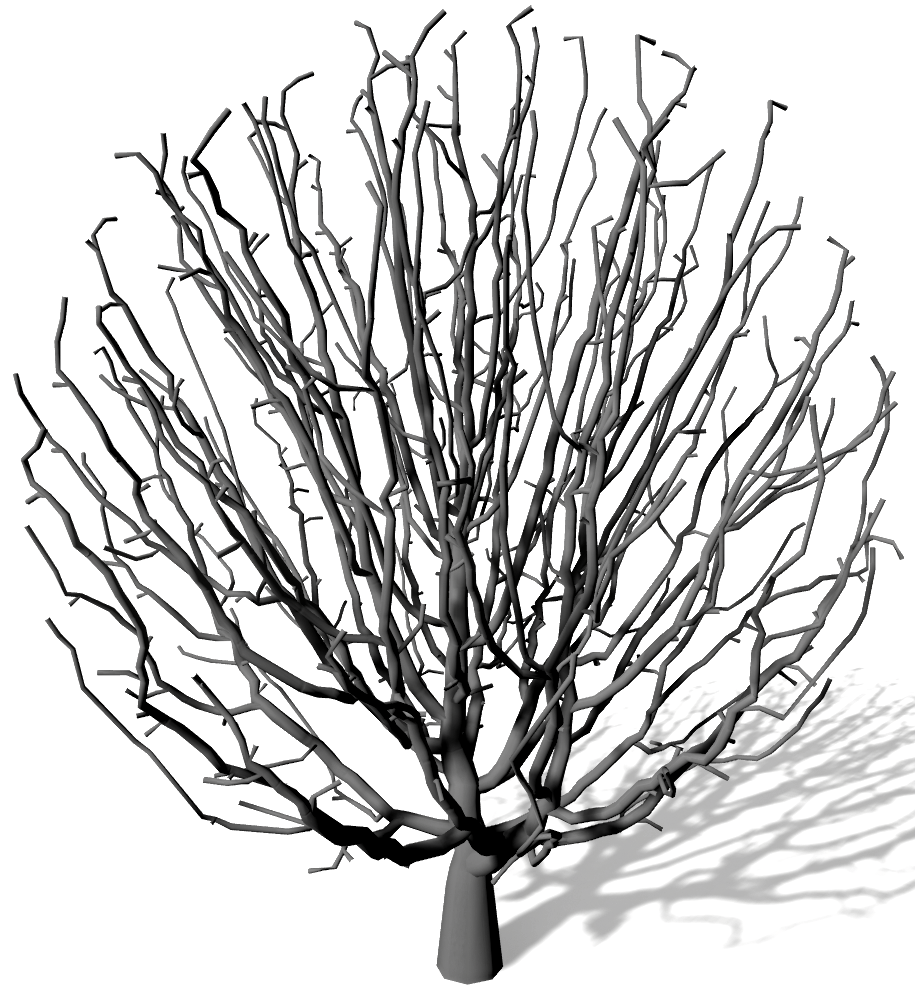
\includegraphics[height=.21\textheight]{images/SCA_Einfluss_Sphere_High.png}
		\caption{Kugelförmig mit Radius $r = 500$, $N = 10000$}
		\label{subfig:SCA_Einfluss_Sphere_High}
	\end{subfigure}	
	\begin{subfigure}[t]{.45\textwidth}
		\centering
		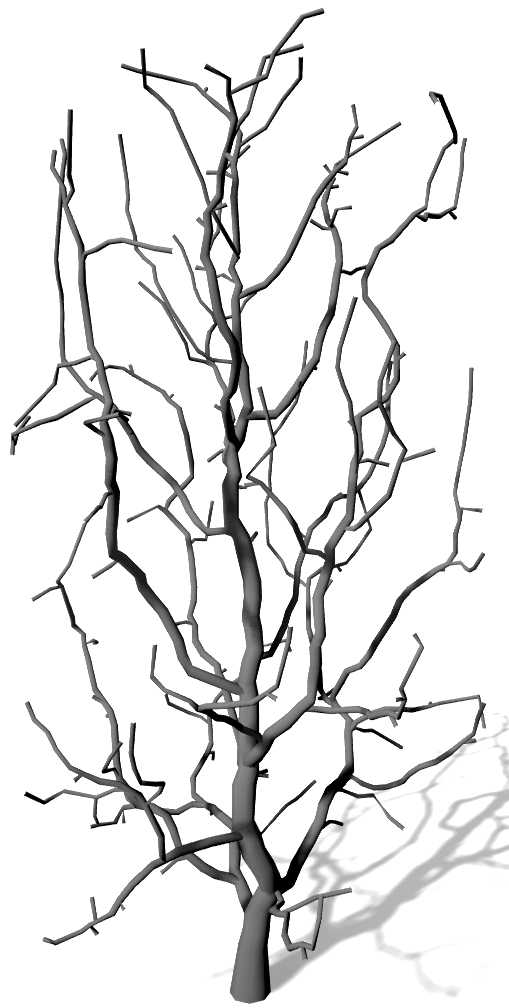
\includegraphics[height=.21\textheight]{images/SCA_Einfluss_Cylinder_Low.png}
		\caption{Zylinderförmig mit Höhe $h=1000$ und Radius $r_z = 300$, $N = 1000$}
		\label{subfig:SCA_Einfluss_Cylinder_Low}
	\end{subfigure}
	\hspace{.05\linewidth}
	\begin{subfigure}[t]{.45\textwidth}
		\centering
		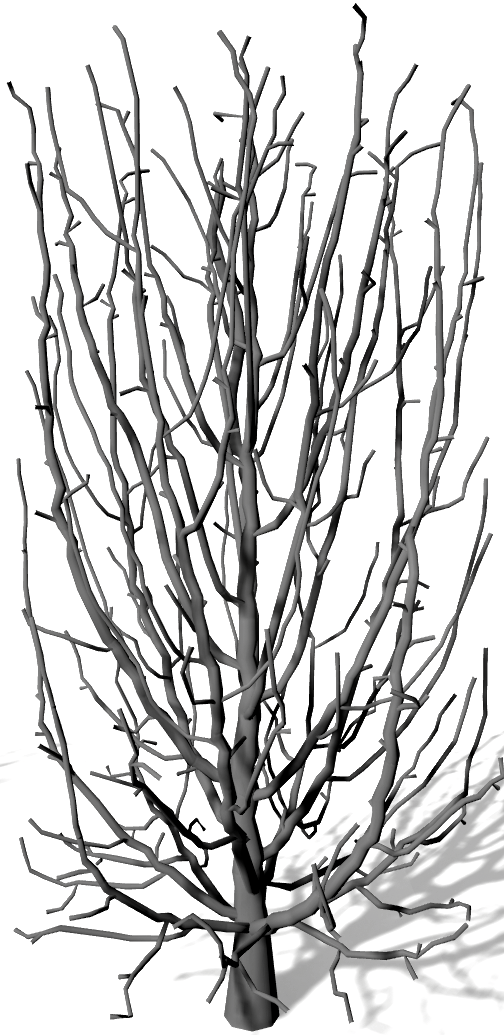
\includegraphics[height=.21\textheight]{images/SCA_Einfluss_Cylinder_High.png}
		\caption{Zylinderförmig mit Höhe $h=1000$ und Radius $r_z = 300$, $N = 10000$}
		\label{subfig:SCA_Einfluss_Cylinder_High}
	\end{subfigure}
	\caption{Wirkung der Anzahl der Einflusspunkte $n$ und der Form des Einflussbereichs auf die generierte Baumstruktur. Eigene Abbildungen.}
	\label{fig:SCA_Einfluss}
\end{figure}
 
 \begin{figure} [hbtp]
 	\centering
 	\begin{subfigure}[t]{.45\textwidth}
 		\centering
 		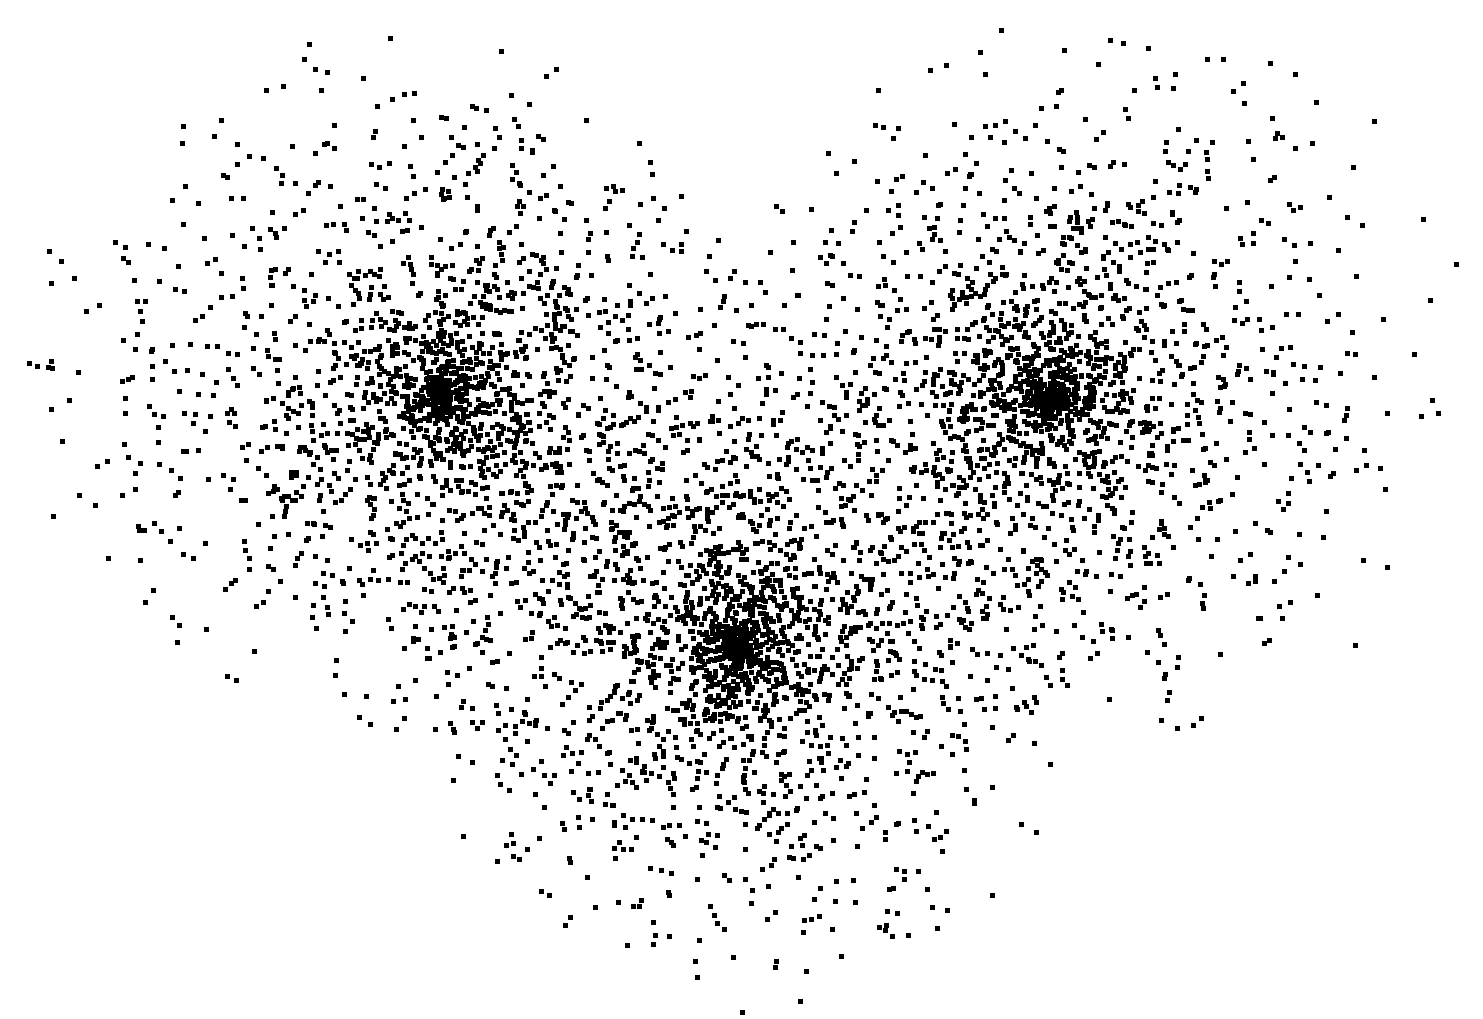
\includegraphics[height=.21\textheight]{images/SCA_MultipleSpheres_Points.png}
 		\caption{Punktewolke.}
 		\label{subfig:SCA_MultipleSpheres_Points}
 	\end{subfigure}
 	\hspace{.05\linewidth}
 	\begin{subfigure}[t]{.45\textwidth}
 		\centering
 		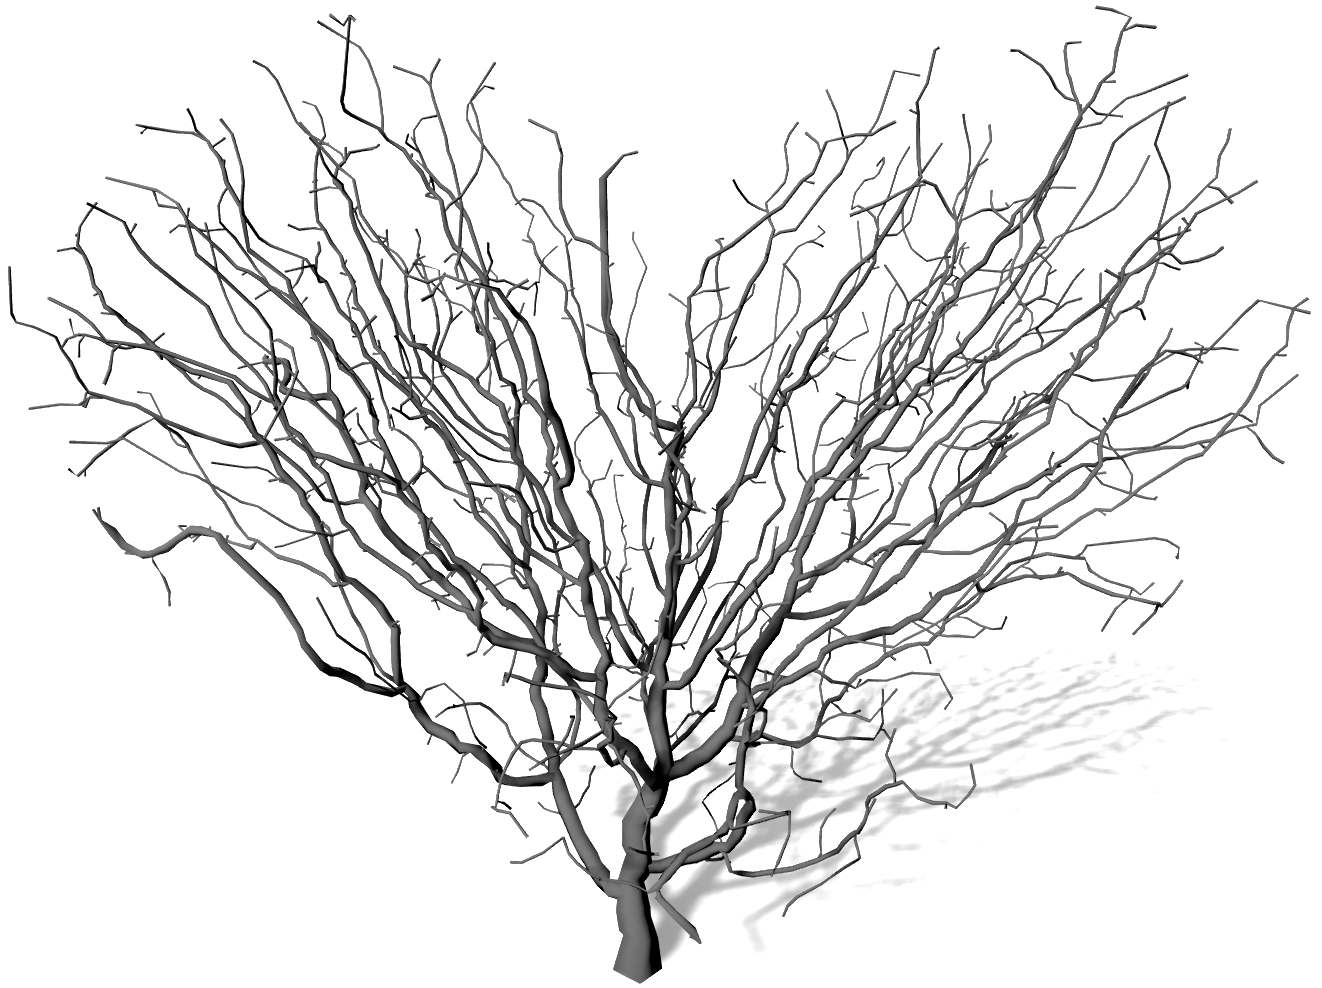
\includegraphics[height=.21\textheight]{images/SCA_MultipleSpheres_Grown.png}
 		\caption{Resultierende Baumstruktur.}
 		\label{subfig:SCA_MultipleSpheres_Grown}
 	\end{subfigure}	
 	\caption{Verbindung von drei kugelförmigen Einflussbereichen zu einem Bereich. Die Kugeln haben jeweils den Radius $r=500$ und $N=2000$. Eigene Abbildungen.}
 	\label{fig:SCA_MultipleSpheres}
 \end{figure}
 
\subsection{Wachstumsparameter}

Bei den Parametern, welche sich direkt auf die Positionierung neuer Knoten auswirken, handelt es sich um Minimalradius, Einflussradius, Schrittweite, Tropismus, Maximale Zweigtiefe, gewichtetes Wachstum, den maximalen Grad eines Knotens und die maximale Anzahl von durchgeführten Iterationen.

\paragraph{Minimalradius und Einflussradius}

Der Minimalradius $d_k$ hat eine ähnliche Wirkung auf eine generierte Baumstruktur wie die Anzahl der Einflusspunkte $N$. Je höher der Minimalradius $d_k$, desto weniger Abzweigungen werden gebildet, da nach der Bildung eines neuen Astsegments Einflusspunkte entfernt werden, die zuvor eine solche Abzweigung bewirkt hätten. Die Baumkrone erscheint spärlicher bewachsen, die entstandenen Äste sind jedoch kurvenreicher, da auf die wenigen wachsenden Äste mehr Einflusspunkte einwirken -- das Entfernen oder Hinzufügen einzelner Einflusspunkte hat somit nur eine kleine Auswirkung auf die Position eines in der nächsten Iteration neu hinzugefügten Astsegments. \cite[S.3]{SpaceColonizationAlgorithm:07}

Je kleiner der Einflussradius $d_i$, desto knorriger wirkt ein Baum, da Astsegmente in jedem Iterationsschritt in den Wirkungsbereich eines Einflusspunktes geraten und im nächsten Schritt wieder verlassen. \cite[S.4]{SpaceColonizationAlgorithm:07}

Abbildung \ref{fig:SCA_KDRI} zeigt Beispiele der Wirkung unterschiedlicher Werte für Einflussradius und Minimalradius.

\begin{figure} [hbtp]
	\centering
	\begin{subfigure}[t]{.45\textwidth}
		\centering
		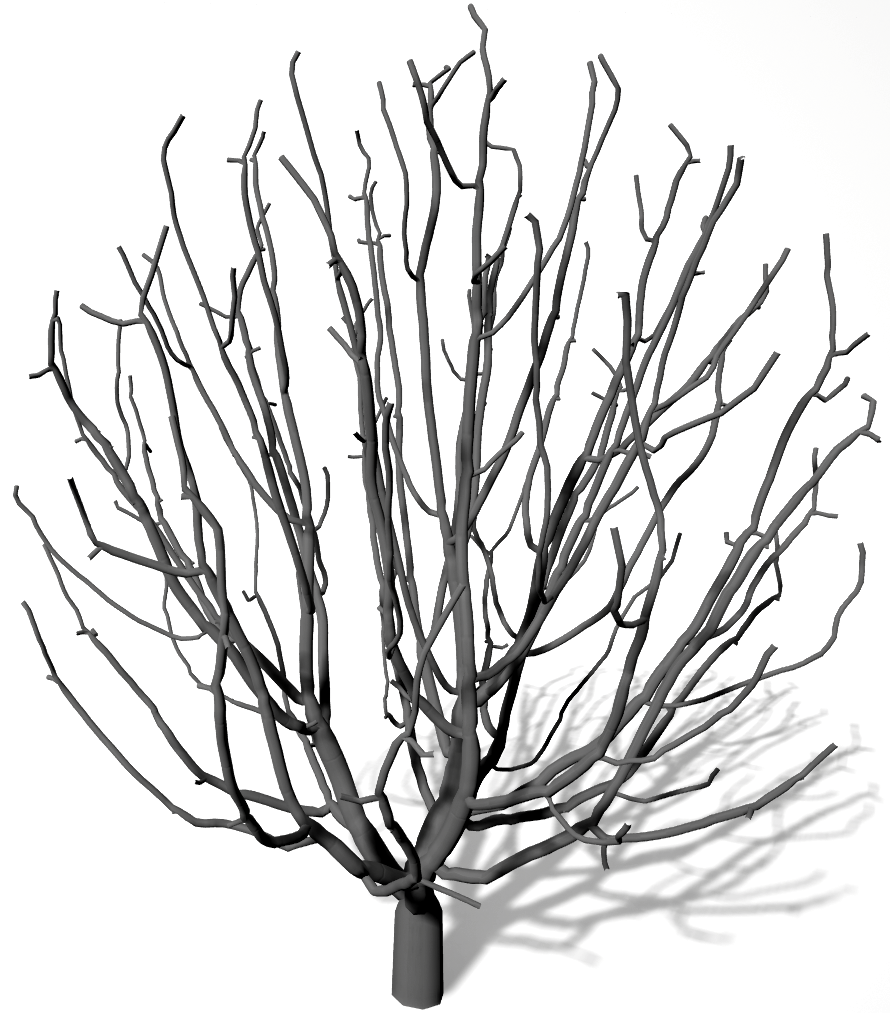
\includegraphics[height=.21\textheight]{images/SCA_KDRI_LowKD_LowRI.png}
		\caption{$d_k = 80$, $d_i = 150$}
		\label{subfig:SCA_KDRI_LowKD_LowRI}
	\end{subfigure}
	\hspace{.05\linewidth}
	\begin{subfigure}[t]{.45\textwidth}
		\centering
		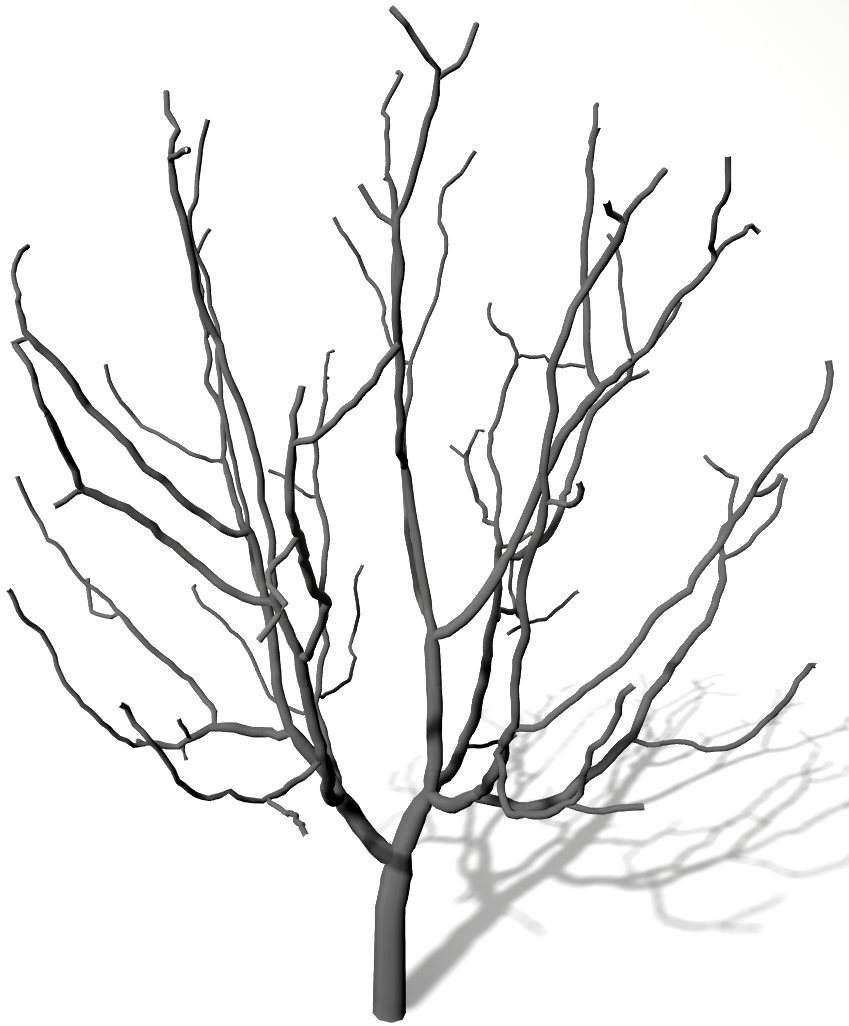
\includegraphics[height=.21\textheight]{images/SCA_KDRI_HighKD_LowRI.png}
		\caption{$d_k = 130$, $d_i = 150$}
		\label{subfig:SCA_KDRI_HighKD_LowRI}
	\end{subfigure}	
	\begin{subfigure}[t]{.45\textwidth}
		\centering
		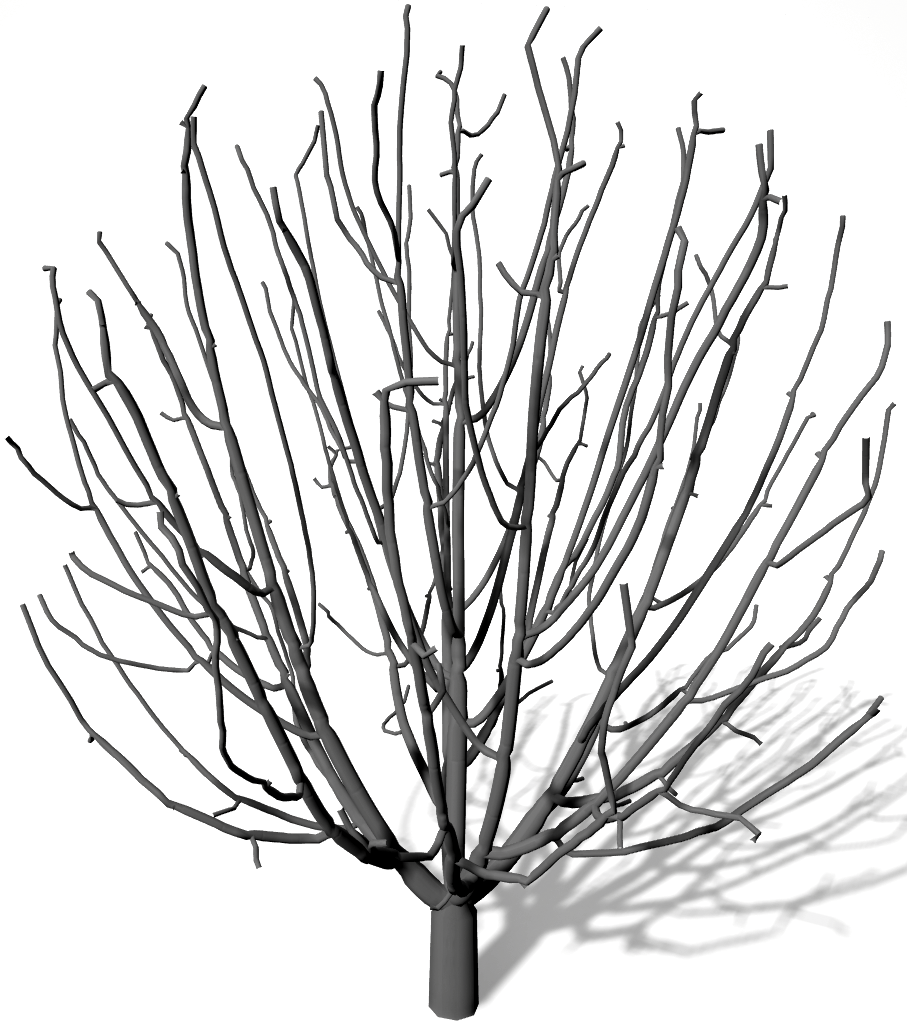
\includegraphics[height=.21\textheight]{images/SCA_KDRI_LowKD_HighRI.png}
		\caption{$d_k = 80$, $d_i = 1000$}
		\label{subfig:SCA_KDRI_LowKD_HighRI}
	\end{subfigure}
	\hspace{.05\linewidth}
	\begin{subfigure}[t]{.45\textwidth}
		\centering
		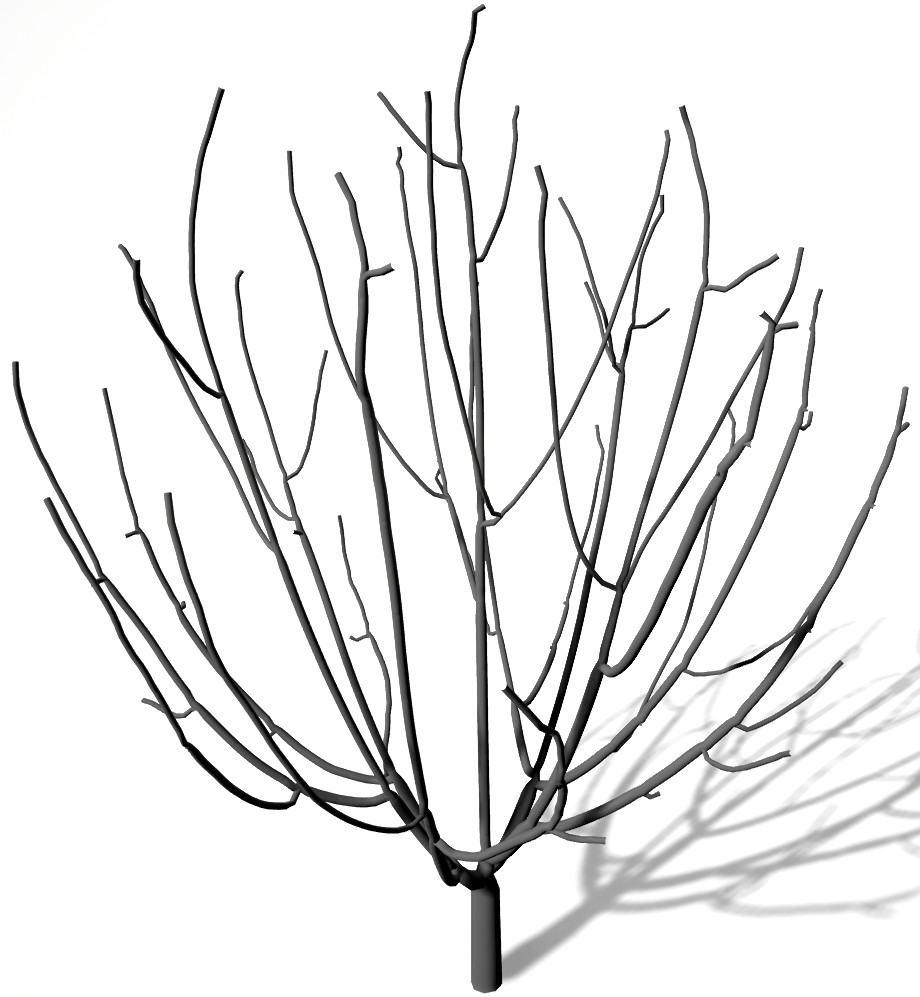
\includegraphics[height=.21\textheight]{images/SCA_KDRI_HighKD_HighRI.png}
		\caption{$d_k = 130$, $d_i = 1000$}
		\label{subfig:SCA_KDRI_HighKD_HighRI}
	\end{subfigure}
	\caption{Wirkung von Einflussradius $d_i$ und Minimalradius $d_k$ auf die generierte Baumstruktur. Es wurde die Schrittweite $D = 10$ verwendet. Eigene Abbildungen.}
	\label{fig:SCA_KDRI}
\end{figure}

\paragraph{Tropismus, maximale Zweigtiefe, maximaler Grad und gewichtetes Wachstum}

Ebenso wie bei der Implementierung von L-Systemen kann der Einfluss eines Tropismusvektors $\overrightarrow{T}$ das Wachstumsverhalten der Space-Colonization Implementierung bei gleichen Parameterwerten stark in eine bestimmte Richtung beeinflussen. Werte auf der horizontalen Ebene erwecken den Anschein von Einwirkung durch Wind. Positive Werte auf der Z-Achse entsprechen dem Streben einer Pflanze der Sonnenposition entgegen zu wachsen, negative Werte auf der Z-Achse simulieren die Einwirkung auf das Wachstum durch Gravitation. \cite[S.5]{SpaceColonizationAlgorithm:07}

Die maximale Zweigtiefe $max_Z$ begrenzt die Anzahl der Abzweigungen, die von dem Wurzel-Astsegment ausgehend zu jedem Astsegment ohne Nachfolger gebildet werden können. Bei niedrigen Werten führt dies zur Bildung weniger, kurvenförmiger Astsegmente.

Der maximale Grad $max_{grad}$ begrenzt die Anzahl der Abzweigungen, die von einem einzelnen Astsegment ausgehen können. Da Astsegmente nur in sehr dichten Baumstrukturen -- Strukturen mit vielen Einflusspunkten und einem niedrigen Minimalradius -- mehr als zwei Nachfolger bilden, hat dieser Parameter eine eingeschränkte visuelle Einwirkung. In dichten Baumstrukturen ermöglicht er es jedoch, bei minimaler visueller Einwirkung, die Anzahl der erstellten Vertizes zu begrenzen. Die Wahl von $max_{grad} = 1$ sorgt für die Bildung eines durchgängigen, in sich verdrehten Astes ohne Abzweigungen.

In Abbildung \ref{fig:SCA_Sonst} werden Beispiele für die Wirkung der beschriebenen Parameter gezeigt.

\begin{figure} [hbtp]
	\centering
	\begin{subfigure}[t]{.45\textwidth}
		\centering
		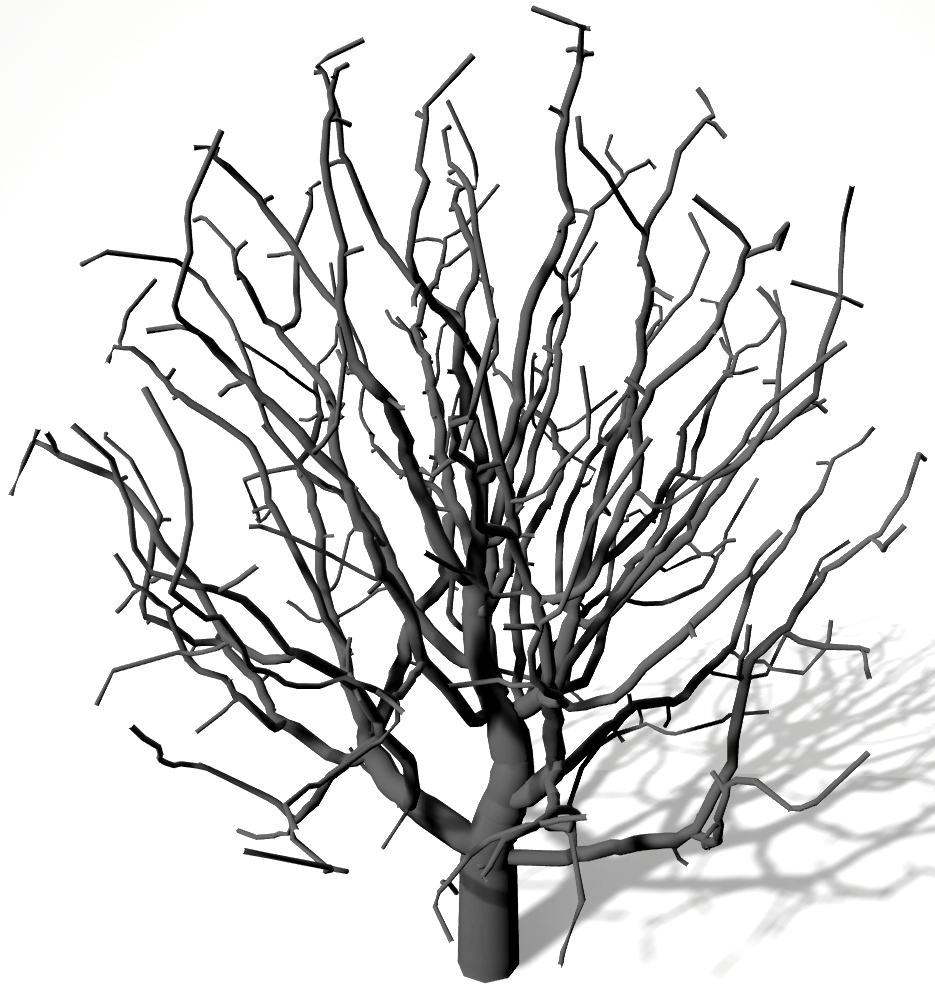
\includegraphics[height=.21\textheight]{images/SCA_Sonst_Ursprung.png}
		\caption{$d_k = 60$, $d_i = 150$, $\protect\overrightarrow{T} = (0,0,0.2)$, $r = 600$, $N = 2000$, $max_Z = 20$, $max_{grad} = 20$, kein gewichtetes Wachstum.}
		\label{subfig:SCA_Sonst_Ursprung}
	\end{subfigure}
	\hspace{.05\linewidth}
	\begin{subfigure}[t]{.45\textwidth}
		\centering
		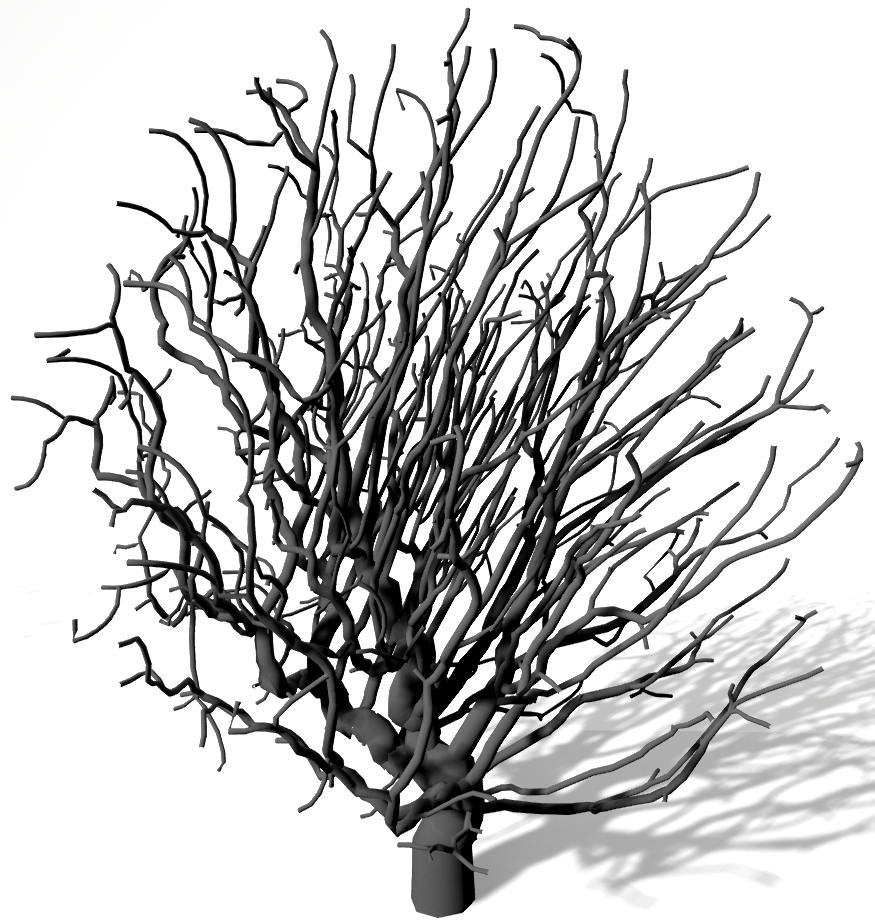
\includegraphics[height=.21\textheight]{images/SCA_Sonst_Tropism_Wind.png}
		\caption{$\protect\overrightarrow{T} = (0,0.8,0)$}
		\label{subfig:SCA_Sonst_Tropism_Wind}
	\end{subfigure}	
	\begin{subfigure}[t]{.45\textwidth}
		\centering
		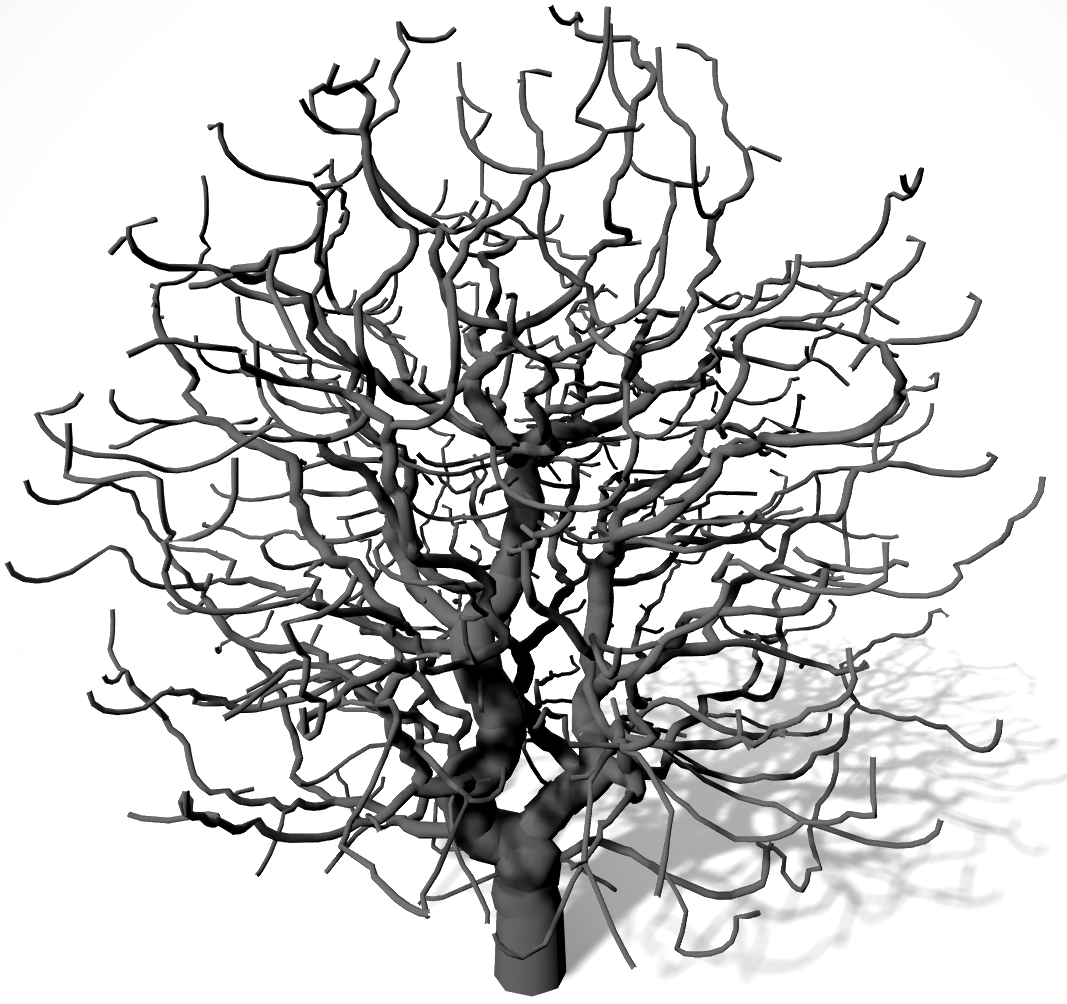
\includegraphics[height=.21\textheight]{images/SCA_Sonst_Tropism_Grav.png}
		\caption{$\protect\overrightarrow{T} = (0,0,-0.8)$}
		\label{subfig:SCA_Sonst_Tropism_Grav}
	\end{subfigure}
	\hspace{.05\linewidth}
	\begin{subfigure}[t]{.45\textwidth}
		\centering
		\includegraphics[height=.21\textheight]{images/SCA_Sonst_Zweigtiefe.png}
		\caption{$max_Z = 2$}
		\label{subfig:SCA_Sonst_Zweigtiefe}
	\end{subfigure}
	\begin{subfigure}[t]{.45\textwidth}
		\centering
		\includegraphics[height=.21\textheight]{images/SCA_Sonst_Grad.png}
		\caption{$max_{grad} = 1$}
		\label{subfig:SCA_Sonst_Grad}
	\end{subfigure}
	\begin{subfigure}[t]{.45\textwidth}
		\centering
		\includegraphics[height=.21\textheight]{images/SCA_Sonst_Grad2.png}
		\caption{$max_{grad} = 2$}
		\label{subfig:SCA_Sonst_Grad}
	\end{subfigure}
	\caption{Wirkung von Tropismus $\protect\overrightarrow{T}$, maximaler Zweigtiefe $max_Z$ und maximalem Knotengrad $max_{grad}$ auf die generierte Baumstruktur. Falls nicht weiter angegeben, wurden die in Abbildung \ref{subfig:SCA_Sonst_Ursprung} angegebenen Parameterwerte verwendet. Eigene Abbildungen.}
	\label{fig:SCA_Sonst}
\end{figure}
 
\paragraph{Schrittweite und maximale Anzahl durchzuführender Iterationen}

Je höher die Schrittweite $D$, desto knorriger wirkt ein Baum -- ähnlich dem Einflussradius -- da ein Astsegment in jedem Schritt Einflussradien betritt und verlässt oder ein neues Astsegment auf der gegenüberliegenden Seite eines Einflusspunktes gebildet wird und von diesem nun aus der entgegengesetzten Richtung beeinflusst wird. Weiterhin besitzen die Äste scharfe Kanten, da aufgrund der größeren Schrittweite weniger Vertizes generiert werden. Die Wahl einer niedrigen Schrittweite führt zur Bildung von Ästen mit leichten Kurven.

Die maximale Anzahl durchzuführender Iterationen $N_I$ beschränkt die Zahl von Space-Colonization Iterationen, die durchgeführt werden sollen. Die bisher gezeigten Beispiele wurden mit $N_I = 400$ durchgeführt und vor Erreichen dieser Zahl abgebrochen. Bei Festlegung niedrigerer Zahlen kann das Wachstum des Baumes beschränkt oder das Wachstumsverhalten im Laufe der Iterationen beobachtet werden.

Abbildung \ref{fig:SCA_SI} zeigt die Auswirkungen verschiedener Werte für die Schrittweite und die maximale Anzahl durchzuführender Iterationen bei gleichbleibender Verteilung der Einflusspunkte.

\begin{figure} [hbtp]
	\centering
	\begin{subfigure}[t]{.45\textwidth}
		\centering
		\includegraphics[height=.21\textheight]{images/SCA_SI_SchrittweiteHigh.png}
		\caption{$d_k = 100$, $d_i = 150$, $D = 50$, $N_I = 400$}
		\label{subfig:SCA_SI_SchrittweiteHigh}
	\end{subfigure}
	\hspace{.01\linewidth}
	\begin{subfigure}[t]{.45\textwidth}
		\centering
		\includegraphics[height=.21\textheight]{images/SCA_SI_SchrittweiteLow.png}
		\caption{$D = 5$}
		\label{subfig:SCA_SI_SchrittweiteLow}
	\end{subfigure}	
	\begin{subfigure}[t]{.2\textwidth}
		\centering
		\includegraphics[height=.11\textheight]{images/SCA_SI_Iterationen10.png}
		\caption{$D = 20$, $N_I = 10$}
		\label{subfig:SCA_SI_Iterationen10}
	\end{subfigure}
	\begin{subfigure}[t]{.2\textwidth}
		\centering
		\includegraphics[height=.11\textheight]{images/SCA_SI_Iterationen20.png}
		\caption{$N_I = 20$}
		\label{subfig:SCA_SI_Iterationen20}
	\end{subfigure}
	\begin{subfigure}[t]{.2\textwidth}
		\centering
		\includegraphics[height=.21\textheight]{images/SCA_SI_Iterationen40.png}
		\caption{$N_I = 40$}
		\label{subfig:SCA_SI_Iterationen40}
	\end{subfigure}
	\begin{subfigure}[t]{.35\textwidth}
		\centering
		\includegraphics[height=.21\textheight]{images/SCA_SI_Iterationen80.png}
		\caption{$N_I = 80$}
		\label{subfig:SCA_SI_Iterationen80}
	\end{subfigure}
	\caption{Wirkung von Schrittweite $D$ und maximaler Anzahl von Iterationen $N_I$ auf die generierte Baumstruktur. Eigene Abbildungen.}
	\label{fig:SCA_SI}
\end{figure}


\paragraph{Gewichtetes Wachstum}

Gewichtetes Wachstum erhöht die Wachstums-Schrittweite der Astsegmente in Abhängigkeit von der Zweigtiefe. Dies führt zu der erkennbaren Bildung eines Stammes und den davon abzweigenden Hauptästen. 

Die Einstellung erzielt den besten visuellen Eindruck in bestimmten Situationen: Bei Anwendung des Algorithmus auf große Werte für den Radius des Einflussbereichs $r$, der Anzahl von Einflusspunkten $N$, dem Einflussradius $d_i$ und bei einer Begrenzung des maximalen Anzahl durchzuführender Iterationen $N_I$, sodass die Baumstruktur nur einen Teil des Einflussbereichs ausfüllen kann. Dies erweckt den Anschein eines Baumes, dessen Wachstum noch nicht beendet ist.

Abbildung \ref{fig:SCA_GewWachstum} zeigt ein Beispiel für die Anwendung von gewichtetem Wachstum in der beschriebenen Situation.

\begin{figure} [hbtp]
	\centering
	\begin{subfigure}[t]{.45\textwidth}
		\centering
		\includegraphics[height=.3\textheight]{images/SCA_GewWachstum_Off.png}
		\caption{$N = 5000$, $r = 1000$, $N_I = 50$, $d_k = 50$, $d_i = 1000$, $D = 15$, $\protect\overrightarrow{T} = (0,0,0.7)$, kein gewichtetes Wachstum.}
		\label{subfig:SCA_GewWachstum_Off}
	\end{subfigure}
	\hspace{.05\linewidth}
	\begin{subfigure}[t]{.45\textwidth}
		\centering
		\includegraphics[height=.3\textheight]{images/SCA_GewWachstum_On.png}
		\caption{Mit gewichtetem Wachstum.}
		\label{subfig:SCA_GewWachstum_On}
	\end{subfigure}	
	\caption{Wirkung von gewichtetem Wachstum auf die generierte Baumstruktur. Eigene Abbildungen.}
	\label{fig:SCA_GewWachstum}
\end{figure}


\section{Effizienz}

Die Effizienz einer Software ist ihre Fähigkeit, mit den durch das Betriebssystem bereitgestellten Ressourcen ein bestimmtes Leistungsniveau zu erzielen. \cite[S.259]{Softwaremanagement:98} In Hinsicht auf prozedurale Generierung muss auf zwei wesentliche Punkte geachtet werden: Die Generierungszeit und das Laufzeitverhalten.

\subsection{Generierungszeit}

Die Zeit welche benötigt wird um eine Baumstruktur aufzubauen wird als Generierungszeit bezeichnet und wird bei den Implementierungen durch die vorgestellten Parameter beeinflusst. Mithilfe des Unreal Engine Profilers wurde die Ausführungszeit bestimmter Funktionen oder Funktionsabschnitte gemessen um die Abhängigkeiten zwischen Parametern und Generierungszeit zu bestimmen. \cite{Profiling:15}

\paragraph{L-System-Actor}

Die Generierungszeit der L-System Implementierung hängt linear von den durch die Turtle-Interpretation ausgeführten Bewegungen und Rotationen ab und macht diese somit abhängig von der Anzahl der Ableitungen sowie den angegebenen Produktionsregeln. Je öfter ein Axiom abgeleitet wird und je mehr Rotations- und Bewegungsaktionen in den Nachfolgern der Produktionsregeln angegeben sind, desto mehr Aktionen enthält die zu interpretierende Zeichenkette. 

\paragraph{Space-Colonization-Actor}

Die Generierungszeit der Space-Colonization Implementierung wird durch eine Vielzahl von Parametern festgelegt, welche die Anzahl der Einflusspunkte, wachsenden Astsegmente und durchzuführenden Iterationen beeinflussen. In einer Iteration wird jeder Einflusspunkt daraufhin überprüft, ob sich mindestens einer der wachsenden Astsegmente in seinem Einflussradius befindet. Falls dies zutrifft wird zusätzlich die Liste der Astsegmente im Einflussradius daraufhin überprüft, welches Segment den geringsten Abstand besitzt.

Die eingeführte Bedingung $max_{NG}$ -- die maximale Anzahl von Iterationen, in welchen einem Astsegment kein neuer Nachfolger hinzugefügt wurde -- begrenzt die Anzahl der aktuell wachsenden Astsegmente und konnten somit erfolgreich zur Verringerung der Generierungszeit eingesetzt werden, ohne die resultierende Baumstruktur visuell erkennbar zu verändern. 

Abbildung \ref{fig:SCA_maxNG} zeigt zwei mit denselben Parametern generierten Space-Colo\-ni\-za\-tion Baumstrukturen, lediglich $max_{NG}$ wurde angepasst. Die Generierungszeit der Baumstruktur aus Abbildung \ref{subfig:SCA_maxNG_1000} beträgt ungefähr das fünffache der Generierungszeit des Modells aus Abbildung \ref{subfig:SCA_maxNG_2}. Die Messung der Generierungszeit fand unter gleichbleibenden Bedingungen auf einem Rechner mit $3.3GHz$ Prozessor statt. 

\begin{figure} [hbtp]
	\centering
	\begin{subfigure}[t]{.45\textwidth}
		\centering
		\includegraphics[height=.2\textheight]{images/SCA_maxNG_2.png}
		\caption{$N = 5000$, $r = 1000$, $N_I = 1000$, $d_k = 100$, $d_i = 250$, $D = 20$, $\protect\overrightarrow{T} = (0,0,0.2)$. \\ $max_{NG} = 2$, $Generierungszeit = 1.12 s$.}
		\label{subfig:SCA_maxNG_2}
	\end{subfigure}
	\hspace{.05\linewidth}
	\begin{subfigure}[t]{.45\textwidth}
		\centering
		\includegraphics[height=.2\textheight]{images/SCA_maxNG_1000.png}
		\caption{$max_{NG} = 1000$, $Generierungszeit = 6.08 s$.}
		\label{subfig:SCA_maxNG_1000}
	\end{subfigure}	
	\caption{Einfluss von $max_{NG}$ auf die Generierungszeit. Die Messungen der Generierungszeit fanden unter gleichbleibenden Bedingungen statt. Eigene Abbildungen.}
	\label{fig:SCA_maxNG}
\end{figure}

\subsection{Laufzeitverhalten}

Das Laufzeitverhalten entspricht in diesem Fall der Anzahl von Bildern (engl.: Frames), die pro Sekunde produziert werden können, auch als Bildrate (engl.: Frames per second oder fps) bezeichnet. In Hinsicht auf die generierten Baumstrukturen ist das Laufzeitverhalten abhängig von der dargestellten Geometrie, da eine Grafikkarte lediglich eine begrenzte Menge Vertexdaten pro Sekunde verarbeiten und darstellen kann. Eine Verbesserung des Laufzeitverhaltens wird durch eine Reduktion der Vertexmenge einer generierten Baumstruktur erreicht.

Das Laufzeitverhalten muss stets gegen die Qualität der zu generierenden Modelle abgewägt werden -- eine Verringerung der Vertexdaten führt zwar zu einer höheren Bildrate, im Gegenzug jedoch auch zu einer niedrigeren visuellen Modellqualität. \cite[S.5]{Deussen:05}

\paragraph{L-System-Actor}

Die Vertexanzahl eines durch ein L-System generierten Baummodells wird durch die Anzahl der Schritte bestimmt, welche von der Turtle-Interpretation durchgeführt werden und ist somit abhängig von der Anzahl an Ableitungen und den definierten Produktionsregeln. 

\paragraph{Space-Colonization-Actor}

Die Anzahl von Vertizes, welche durch die Space-Colonization Implementierung generiert werden, hängt von Parametern ab, welche die Anzahl der erstellen Astsegmente beeinflussen. Insbesondere eine Verringerung der Schrittweite und des Minimalradius tragen zu einer Erhöhung der Anzahl an generierten Astsegmenten bei.

\paragraph{Modellgenerierungssystem}

Das Modellgenerierungssystem bietet drei Parameter zur Anpassung der Modellqualität: die minimale und maximale Anzahl von Zylindersektionen sowie den Kurvenreduktionswert, die sich auf generierte Bäume beider Implementierungen anwenden lassen.

Für jedes Astsegment wird die Anzahl an Zylindersektionen festgelegt, indem, abhängig von der Zweigtiefe des Segments, zwischen der minimalen und maximalen Anzahl $n_{min}$ und $n_{max}$ linear interpoliert wird. Das Resultat ist, dass Astsegmente mit einer hohen Zweigtiefe und geringem Radius mit weniger Vertizes dargestellt werden als Astsegmente mit einer niedrigen Zweigtiefe und großem Radius.

Der Kurvenreduktionswert $max_K$ reduziert die Zahl der Astsegmente, indem Segmente, die in einem geringen Winkel voneinander abstehen, zusammen gefasst werden. Die geringere Astsegmentanzahl führt zu einer Verringerung der Vertexanzahl.

\begin{figure} [hbtp]
	\centering
	\begin{subfigure}[t]{.45\textwidth}
		\centering
		\includegraphics[height=.2\textheight]{images/SCA_Quali_SegmentsLow.png}
		\caption{$n_{min} = 3$, $n_{max} = 5$, $max_K = 1.0$\\ $N_V = 23565$.}
		\label{subfig:SCA_Quali_SegmentsLow}
	\end{subfigure}
	\hspace{.05\linewidth}
	\begin{subfigure}[t]{.45\textwidth}
		\centering
		\includegraphics[height=.2\textheight]{images/SCA_Quali_SegmentsHigh.png}
		\caption{$n_{min} = 8$, $n_{max} = 12$, $max_K = 1.0$\\ $N_V = 54009$.}
		\label{subfig:SCA_Quali_SegmentsHigh}
	\end{subfigure}	
	\begin{subfigure}[t]{.45\textwidth}
		\centering
		\includegraphics[height=.2\textheight]{images/SCA_Quali_CR_Low.png}
		\caption{$n_{min} = 8$, $n_{max} = 12$, $max_K = 0.99$\\ $N_V = 34709$.}
		\label{subfig:SCA_Quali_CR_Low}
	\end{subfigure}
	\hspace{.05\linewidth}
	\begin{subfigure}[t]{.45\textwidth}
		\centering
		\includegraphics[height=.2\textheight]{images/SCA_Quali_CR_High.png}
		\caption{$n_{min} = 8$, $n_{max} = 12$, $max_K = 0.5$\\ $N_V = 14130$.}
		\label{subfig:SCA_Quali_CR_High}
	\end{subfigure}	
	\caption{Einfluss der minimalen und maximalen Anzahl an Zylindersektionen $n_{min}$ und $n_{max}$ sowie des Kurvenreduktionswerts $max_K$ auf die Zahl der generierten Vertizes $N_V$. Die Parameter für die Generierung des zugrunde liegenden graphentheoretischen Baums stimmen überein. Eigene Abbildungen.}
	\label{fig:SCA_Quali}
\end{figure}



\chapter{Zusammenfassung und Ausblick}

Zusammenfassung

\section{Erweiterungen}

\subsection{Texturen}

\subsection{Blätter}

\subsection{Generierung zur Laufzeit}

\subsection{Verteilung}



\bibliographystyle{geralpha}			% Literaturverzeichnis
\bibliography{literatur}     			% BibTeX-File literatur.bib


\newpage
\slidetitle{5. Ergebnisse - L-Systeme}
\subsection{Ergebnisse (2)}





\newpage
\begin{center}
	\vfill
	\begin{minipage}[c]{0.45\textwidth}
		\centering
		\includegraphics[height=.9\textheight]{images/LS_Monopodial_1}
	\end{minipage}
	\hspace{.05\textwidth}	
	\begin{minipage}[c]{0.45\textwidth}
		\centering
		\includegraphics[height=.9\textheight]{images/LS_Monopodial_2}
	\end{minipage}
	\vspace{0.05\textheight}
	
	Monopodiales Wachstum
\end{center}







\newpage
\begin{center}
	\vfill
	\begin{minipage}[c]{0.45\textwidth}
		\centering
		\includegraphics[height=.9\textheight]{images/LS_Sympodial_1}
	\end{minipage}
	\hspace{.05\textwidth}	
	\begin{minipage}[c]{0.45\textwidth}
		\centering
		\includegraphics[height=.9\textheight]{images/LS_Sympodial_2}
	\end{minipage}
	\vspace{0.05\textheight}
	
	Sympodiales Wachstum
\end{center}







\newpage
\begin{center}
	\includegraphics[height=.9\textheight]{images/LS_Ternary_2}
	
	Ternäre Verzweigungen ohne Tropismus
\end{center}






\newpage
\begin{center}
	\includegraphics[height=.9\textheight]{images/LS_Ternary_2_Tropism}

	Ternäre Verzweigungen mit Tropismus: $\overrightarrow{T} = (0, -0.5, -1)^T$, $e = 0.5$	
\end{center}








\newpage
\slidetitle{5. Ergebnisse - Space Colonization Algorithmus}
\begin{center}
	\vfill
	\begin{minipage}[c]{0.45\textwidth}
		\centering
		\includegraphics[height=.9\textheight]{images/SCA_Einfluss_Cylinder_High}
	\end{minipage}
	\hspace{.05\textwidth}	
	\begin{minipage}[c]{0.45\textwidth}
		\centering
		\includegraphics[height=.9\textheight]{images/SCA_Einfluss_Cylinder_Low}
	\end{minipage}
	\vspace{0.05\textheight}

	Form des Einflussbereiches und Anzahl der Einflusspunkte
\end{center}






\newpage
\begin{center}
	\vfill
	\begin{minipage}[c]{0.45\textwidth}
		\centering
		\includegraphics[height=.65\textheight]{images/SCA_MultipleSpheres_Points}
	\end{minipage}
	\hspace{.05\textwidth}	
	\begin{minipage}[c]{0.45\textwidth}
		\centering
		\includegraphics[height=.65\textheight]{images/SCA_MultipleSpheres_Grown}
	\end{minipage}
	\vspace{0.1\textheight}

	Zusammenführen mehrerer Einflussbereiche
\end{center}



\newpage
\begin{center}
	\vfill
	\begin{minipage}[c]{0.45\textwidth}
		\centering
		\includegraphics[height=.9\textheight]{images/SCA_KDRI_HighKD_LowRI}
	\end{minipage}
	\hspace{.05\textwidth}	
	\begin{minipage}[c]{0.45\textwidth}
		\centering
		\includegraphics[height=.9\textheight]{images/SCA_KDRI_HighKD_HighRI}
	\end{minipage}
	\vspace{0.05\textheight}
	
	Unterschiedliche Einflussradien
\end{center}





\newpage
\begin{center}
	\vfill
	\begin{minipage}[c]{0.45\textwidth}
		\centering
		\includegraphics[height=.9\textheight]{images/SCA_KDRI_HighKD_LowRI}
	\end{minipage}
	\hspace{.05\textwidth}	
	\begin{minipage}[c]{0.45\textwidth}
		\centering
		\includegraphics[height=.9\textheight]{images/SCA_KDRI_LowKD_LowRI}
	\end{minipage}
	\vspace{0.05\textheight}
	
	Einfluss des Minimalradius
\end{center}




\newpage
\begin{center}
	\vfill
	\begin{minipage}[c]{0.45\textwidth}
		\centering
		\includegraphics[height=.9\textheight]{images/SCA_GewWachstum_Off}
	\end{minipage}
	\hspace{.05\textwidth}	
	\begin{minipage}[c]{0.45\textwidth}
		\centering
		\includegraphics[height=.9\textheight]{images/SCA_GewWachstum_On}
	\end{minipage}
	\vspace{0.05\textheight}
	
	Optimale Verwendung des gewichteten Wachstums
\end{center}

\end{document}
